%Balíčky
\documentclass[a4paper,10pt,twoside]{article}
\usepackage[utf8]{inputenc} %kodovani, abychom mohli jednoduse psat diakriticka pismena
\usepackage[english]{babel}
\usepackage{pdfpages}
\usepackage{pifont}
\usepackage{graphicx} %pro vkladani obrazku
\usepackage{color}
\usepackage{fancyhdr} %zahlavi a zapati
\usepackage{ifpdf}
\usepackage{amssymb}
\usepackage{booktabs}
\usepackage{subfigure}
\usepackage{titlesec}
\usepackage[multiple]{footmisc}
\usepackage{color}       % pro zvýraznění textu barvou
\usepackage{multirow} 
\usepackage{multicol}
\usepackage{amsmath}
\usepackage{sectsty}
\usepackage[justification=centering]{caption}
\usepackage[top=1.5cm, left=2cm, right=2cm, bottom=2cm, headheight=26pt, includeheadfoot]{geometry}
\usepackage[colorlinks=false,urlcolor=black]{hyperref}
\usepackage{xcolor}
\usepackage{listings}
\hypersetup{
    colorlinks=true,
    linkcolor=black,
    filecolor=black,      
    urlcolor=black,
    citecolor=black
}
\allsectionsfont{\rmfamily} 

\sectionfont{\huge}
\subsectionfont{\LARGE}
\subsubsectionfont{\Large}

\def\nazevprace{\Large{Creation of a new GRASS GIS startup mechanism}}
\def\nazevpraceEN{\large{Tvorba nového startovacího mechanismu v prostředí GRASS GIS}}

\begin{document}
\sloppy
\setlength{\parskip}{8pt}

%%  ÚVODNÍ STRÁNKA %%%%%%%%%%%%%%%%%%%%%%%%%%%%%%%%%%%%%%%%%%%%%%

\pagestyle{empty} % vypne číslování stránek na úvodní straně

\begin{center}

\LARGE
\textsc{Czech Technical University in Prague} \\
\textsc{Faculty of civil engineering} \\

\bigskip

\large
\textsc{Department of Geomatics} \\

\vspace{6ex}

\begin{figure}[hbt!] %vlozeni loga
\begin{center}

\includegraphics[width=5.5cm]{../pictures/logo_cvut.png} 
\end{center}
\end{figure}

\vspace{20ex}

\LARGE{MASTER'S THESIS}\\
\bigskip
\bigskip
\textsc{\nazevprace} \\
\smallskip
\textsc{\nazevpraceEN} \\

\mbox{}
\vfill

\normalsize
\textsc{\author} \\
\bigskip
\normalsize
\textrm{Supervisor: Ing. Martin Landa Ph.D.} \\

\vspace{10ex}
\large
\textrm{2020 Prague} \hfill
\textrm{Bc. Linda KLADIVOVÁ} \\

\end{center}

%% 2. STRÁNKA ZŮSTANE PRÁZDNÁ

\newpage ~ \newpage
\thispagestyle{empty}

%% 3. STRÁNKA NA ZADÁNÍ
\begin{figure}
 \centering 
 
\includepdf[pages=-]{../assignment/zadanidp.pdf}
\end{figure}

%% 4. STRÁNKA ZŮSTANE PRÁZDNÁ

\newpage ~ \newpage
\newpage ~ \newpage
\thispagestyle{empty}

%% 5.  STRÁNKA = ČESKÁ A ANGLICKÁ ANOTACE %%%%%%%%%%%%%%%%%%%%%%%%%%%%%%%%%

\renewcommand{\baselinestretch}{1.30} %zvetseni mezery mezi radky


\begin{Large}
\noindent ANNOTATION
\end{Large}

\large
\noindent
The existing GRASS GIS software start-up mechanism could discourage new users from further working with this software or at least make it uncomfortable. This diploma thesis is built on the programming part performed in the summer of 2020 within the international Google Summer of Code program (GSoC) and uses two surveys to evaluate the benefits of significant changes that have taken place. The first part of the work focuses on a survey among intermediate users and compares the startup mechanism of the original GRASS GIS 7.8 version with the new solution introduced after GSoC which during normal startup cancels the concept of the startup window and its role is taken over by Data Catalog. The second part is oriented on newcomers and implements the first-time mode. A survey based on a simple task further examines whether the initial contact of the user with the software when using the first-time mode is more pleasant or not.

\vspace{2ex}
\begin{Large}
\noindent KEYWORDS
\end{Large}

\large
\noindent
\textrm{GUI, GRASS GIS, wxPython, startup, GSoC, first-time user, participatory software development}

\mbox{}
\vfill

\begin{Large}
\noindent ANOTACE
\end{Large} 

\large
\noindent
Dosavadní startovací mechanismus softwaru GRASS GIS mohl odradit nové uživatele od další práce s tímto softwarem nebo ji alespoň znepříjemnit. Cílem této práce je pokračovat v programovací části vytvořenou v létě 2020 v rámci mezinárodního programu Google Summer of Code (GSoC) a pomocí dvou průzkumů vyhodnotit přínos výrazných změn, ke kterým došlo. První část práce se zaměřuje na průzkum mezi středně pokročilými uživateli a porovnává startovací mechanismus původní verze GRASS GIS 7.8 s novým řešením představeným po GSoC, které ruší při běžném startování koncept startovacího okna a tuto roli přebírá Data Catalog. Druhá část se orientuje na nové uživatele a implementuje tzv. "first-time" mód. Průzkumem založeným na jednoduchém úkolu dále zkoumá, zda je počáteční kontakt uživatele se softwarem při využití "first-time" módu příjemnější či nikoliv.

\vspace{2ex}
\begin{Large}
\noindent KLÍČOVÁ SLOVA
\end{Large}

\large
\noindent
\textrm{GUI, GRASS GIS, wxPython, startup, GSoC, vývoj softwaru}


%% 6. STRÁNKA ZŮSTANE PRÁZDNÁ

\newpage ~ \newpage
\thispagestyle{empty}

%% 7. STRÁNKA = DECLARATION OF AUTHORSHIP %%%%%%%%%%%%%%%%%%%%%%%%%%%%%%%%%

\newpage
\mbox{}
\vfill
\begin{Large}
\noindent DECLARATION OF AUTHORSHIP
\end{Large}

I hereby declare that the work presented here is, to the best of my knowledge and belief, the original result of my own investigations, except as acknowledged.  All  direct  or  indirect  sources used are acknowledged as references.
\vspace{3ex}

\noindent In Prague ................................... \hfill ................................................

%% 8. STRÁNKA ZŮSTANE PRÁZDNÁ

\newpage ~ \newpage
\thispagestyle{empty}


%% 9. STRÁNKA = ACKNOWLEDGEMENT %%%%%%%%%%%%%%%%%%%%%%%%%%%%%%%%%

\newpage
\mbox{}
\vfill
\begin{Large}
\noindent ACKNOWLEDGEMENT
\end{Large}

Firstly I would like to thank my parents very much for their support during my studies. Then I would like to express my great thanks to Martin Landa who inspired me and still inspires me a lot on my way of becoming a professional python developer. He was also at the beginning of my participation in the Google Summer of Code program. In the GRASS GIS open-source environment, I met an amazing community of incredibly inspiring people. Among those people, I would like to thank especially Anna and Vaclav Petras who were a great support to me during GSoC and even later on and brought a lot of valuable advice to this work.

%% 10. STRÁNKA ZŮSTANE PRÁZDNÁ

\newpage ~ \newpage
\thispagestyle{empty}


%% 11. a 12. STRÁNKA = OBSAH A SEZNAM OBRAZKU %%%%%%%%%%%%%%%%%%%%%%%%%%%%%%%%%%
\newpage

\tableofcontents %obsah
\newpage
\listoffigures %seznam obrazku

\thispagestyle{empty}
\newcommand{\obrazek}[1]{(viz obr. \ref{#1})} %specialni reference na obrazek

\newpage
\pagestyle{fancy}

%% NASTAVENI VZHLEDU STRANEK (ZAHLAVI A ZAPATI)

% zajistí, že se názvy kapitol a sekcí nebudou sázet velkými písmeny
\renewcommand{\sectionmark}[1]{\markright{\ #1}}

\fancyhf{} % smaže aktuální nastavení záhlaví a zápatí
\renewcommand{\headrulewidth}{0.4pt} % vrchní linka
\renewcommand{\footrulewidth}{0.4pt}  %  spodní linka
\addtolength{\voffset}{-0.4cm}

 %záhlaví
\fancyhead[LE, LO]{{
\includegraphics[width=1cm]{../pictures/logo_cvut.png} }
   {\textsc{\small {CTU in Prague}} }} %logo skoly
\fancyhead[RE, RO]{\nouppercase{\rightmark}}
   
 %zápatí
\fancyfoot[RO, LE]{{\textsc{\small \thepage}}}

\fancypagestyle{plain}{
  \fancyhead{} % na prázdných stránkách nechci záhlaví
  \renewcommand{\headrulewidth}{0pt} % ani linku
}



%% -------<<< Chapter: Introduction >>>-------\\%%%%%%%%%%%%%%%%%%%%%%%%%%%%%%%%%%%%
\newpage
\vspace*{-1cm}
\pagestyle{fancy}
\fancyhead[RE, RO]{\fancyplain{}{\small \sl{Introduction}}}
\section*{Introduction}
\addcontentsline{toc}{section}{Introduction}
\large
\setcounter{page}{13}  % nastaví čítač stránek od stránky Úvod na stránku č. 13



%% -------<<< Chapter 1: State of Art in the version 7.8 >>>-------\\%%%%%%%%%%%%%%%%%%%%%%%%%%%%%%%%%%%%


Changing the startup mechanism, which will make it easier for first-time users to become familiar with GRASS, has been one of the long-term goals of the development community around this software. This whole topic provoked heated discussions mainly because it was not clear whether to keep the startup screen or not.


%% -------<<< Chapter 1: State of Art in the version 7.8 >>>-------\\%%%%%%%%%%%%%%%%%%%%%%%%%%%%%%%%%%%%


\newpage
\vspace*{-1cm}
\fancyhead[RE, RO]{\fancyplain{}{\small \sl{Theory and background information}}}
\section{Theory and background information}
\label{section:explanation}



\subsection{GRASS GIS concepts}
\noindent There are several special concepts and components in the GRASS GIS software that need to be clarified at the outset. We will first explain the concept of data hierarchy in GRASS, which itself includes many other concepts. We will also shed light on the purpose of some GRASS software components arranged chronologically according to the order in which the user encounters them. The description is intentionally related to version 7.8. However, it should be taken into account that there have been significant changes in version 7.9, which change the function of the Startup Screen and Data Catalog in the whole concept of the Startup Mechanism. These changes are clearly shown in the chapter \ref{State of Art} which describes the state of GRASS GIS in version 7.9 after the changes I made during the Google Summer of Code.
Finally, we define the term Startup mechanism, which was introduced for the purposes of this work.

\subsubsection{Data hierarchy in GRASS GIS}
\label{subsection:hierarchy}
\noindent
\large

\noindent While in other software it is usually customary to store work in so-called \textit{projects} in which there are different \textit{map layers} (for more information see the chapter \ref{sec:startup_concepts}), GRASS GIS keeps its own data hierarchy, which has proven very useful over the years, especially for experienced users. Every GRASS GIS user has undoubtedly come across the following terms: Database, Location, Mapset and Maps. These four representations form a tree of rules, which we can see on Figure \ref{fig:grass_data_hierarchy}.

The Database, which is built hierarchically at the top, has the character of a working directory, whose usual name is ``grassdata''. It contains Locations that can have different coordinate systems. Therefore, Maps in the Mapsets contained in a particular Location will always have the same coordinate system.

It is also important to mention that when creating a location, a mapset named PERMANENT is automatically created. Briefly speaking, the PERMANENT mapset is used to store general spatial data which are also accessible but write-projected to other users who are working in the same Location as Database owner. The PERMANENT mapset also holds the default region boundary coordinate values for the whole Location.

In the following text, the elements of the GRASS data hierarchy are marked in italics for greater clarity.

\vspace{0.3cm}
\begin{figure}[hbt!]
\begin{center}
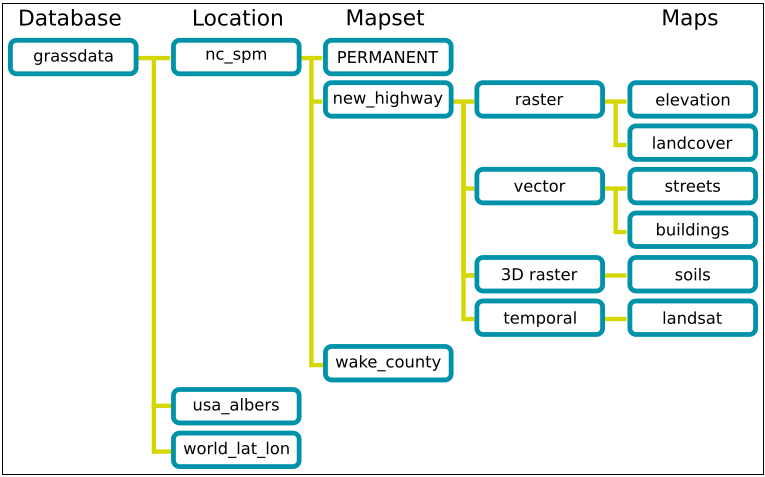
\includegraphics[width=14cm]{../pictures/grass_data_hiearchy.png} 
\caption[GRASS GIS 7 location structure]{GRASS GIS 7 location structure}
\label{fig:grass_data_hierarchy}
\end{center}
\end{figure}

\subsubsection{Startup screen versus splash screen}
\label{subsection:mechanism}
\noindent
\large
First, it is important to distinguish between the terms startup screen and splash screen. As Ed Foster stated in 1996: ``Splash screens, as they are commonly called, are the graphic logos that display while the program is loading and identify the program while reminding you about the software publisher's copyright restrictions." So, it appears before the main software window starts and remains visible for a few seconds. If we try to find articles on the startup screen, we will not be very successful. Nowadays, this topic lives mainly on programming websites such as Stack Overflow. In some software startup screen can mean at the same time a splash screen. However, generally speaking, a startup screen usually requires some initial action from the user to set up the software. 

The startup screen is the first component of the GRASS GIS version 7.8 that the user will meet. It allows us to set all the above-mentioned components except \textit{maps} and, in the case of \textit{locations} and \textit{mapsets}, also manage them in terms of renaming and deleting. The various historical versions of the startup screen can be seen in Figure \ref{fig:verze_startup}. The one on the right corresponds to the version 7.5 (as well as 7.8).

\vspace{0.3cm}
\begin{figure}[hbt!]
\begin{center}
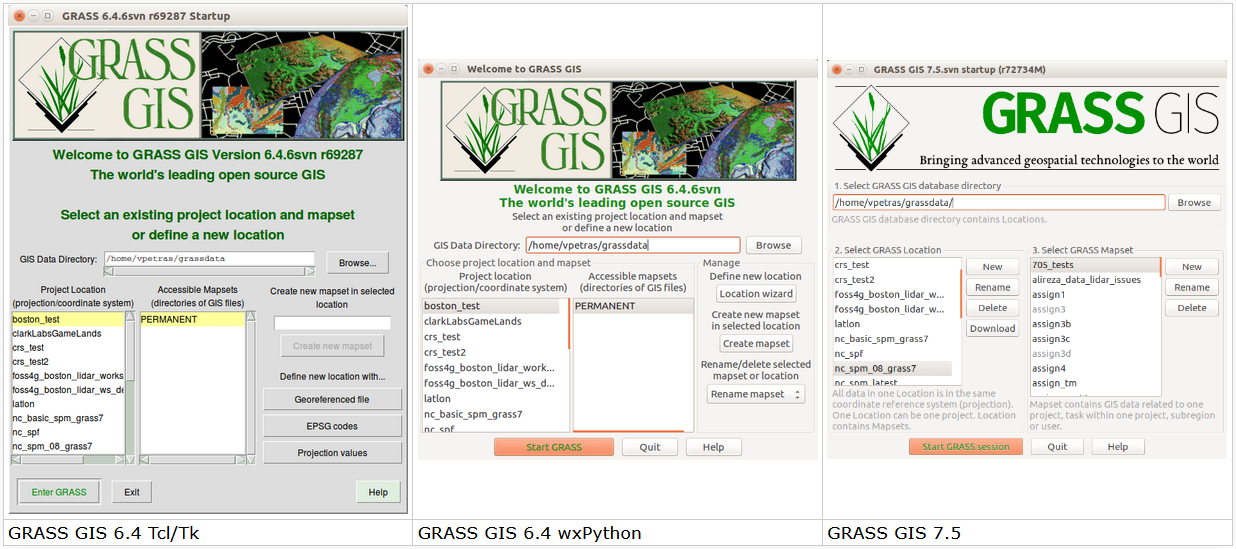
\includegraphics[width=15cm]{../pictures/verze_startup.png} 
\caption[Historical versions of the GRASS startup screen]{Historical versions of the GRASS startup screen}
\label{fig:verze_startup}
\end{center}
\end{figure}

\subsubsection{Location Wizard}
\label{subsection:wizard}
\noindent
\large
Location Wizard is a software component, which has the character of a guide which appears when creating a new \textit{location} - collection of data with common CRS/SRS. Therefore, the main task of the wizard is to define this system. It consists of four consecutive dialog boxes, the one for selecting the coordinate system can be seen in Figure \ref{fig:loc_wizard_sour_pred}.

\vspace{0.3cm}
\begin{figure}[hbt!]
\begin{center}
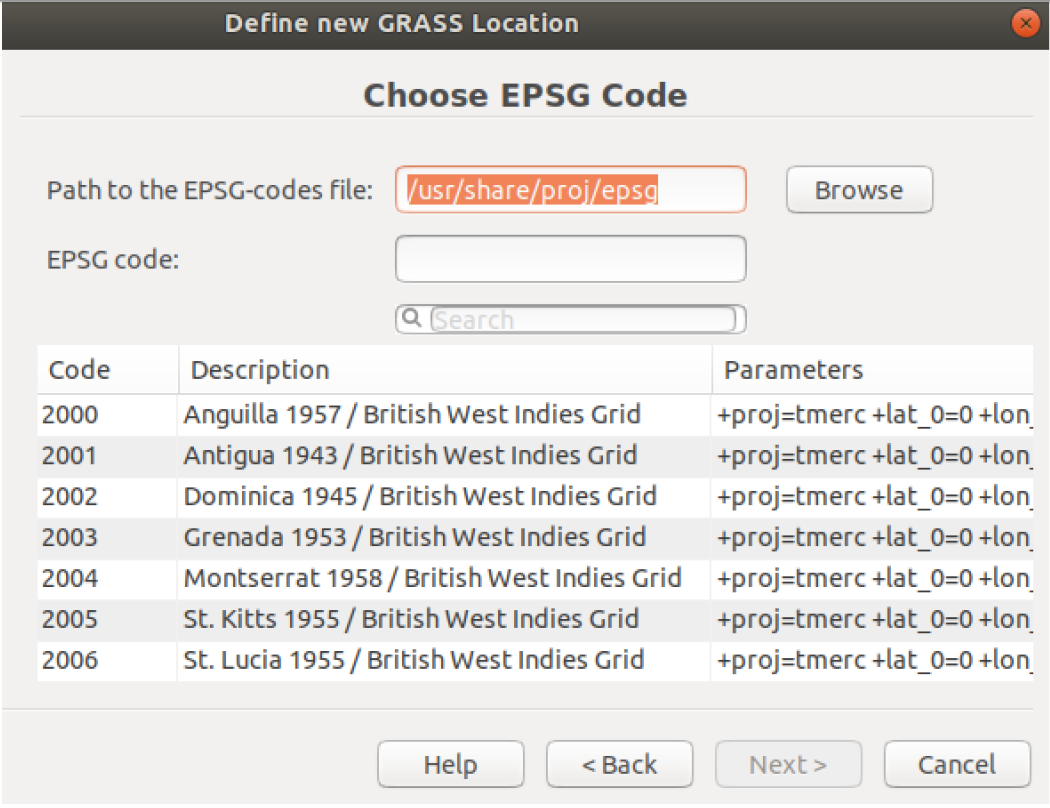
\includegraphics[width=11cm]{../pictures/loc_wizard_sour_pred.png} 
\caption[Choosing EPSG code in Location Wizard in version 7.8]{Choosing EPSG code in Location Wizard in version 7.8 (source: own)}
\label{fig:loc_wizard_sour_pred}
\end{center}
\end{figure}

\newpage
\vspace*{-1cm}
\subsubsection{Layer Manager and Map Window}

\noindent The peculiarity of GRASS GIS is that it does not consist of one software window, as is usually the custom, but directly of two. The topic of connecting Layer Manager with Map Window is, by the way, another of the things that are likely to come, it is also one of the proposed topics on GSoC.

As explained in more detail in the documentation, Layer Manager provides a GUI for creating and managing \textit{maps}. In the image \ref{fig:empty_layers1} we can notice five tabs - Layers, Console, Modules, Data and Python.

In the Layer Manager version 7.8, after running GRASS we first see the Layers tab, which allows layers in Map Display to be switched on and off. After starting the session this tab is empty. The path to the current \textit{mapset} and \textit{location} can be noticed in the top bar in the Map Display window. In this case, the current mapset is called \textit{demomapset} and is located in the location named \textit{fire\_grassdata}. GRASS GIS allows to add more Map Display windows. You can then manage layers in these windows via the Layers tab.
\vspace{0.3cm}
\begin{figure}[hbt!] 
\begin{center}
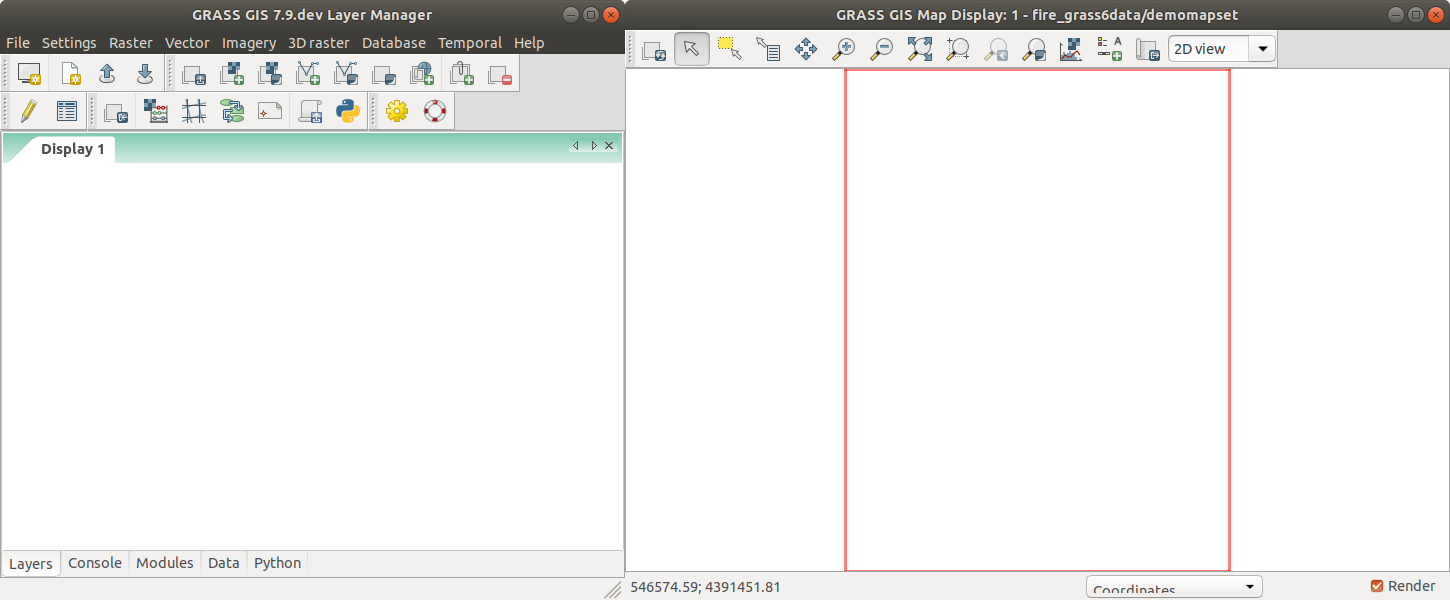
\includegraphics[width=15cm]{../pictures/empty_layers1.png} 
\caption[Layer Manager and Map Window (version before GSoC)]{Layer Manager and Map Window  (version before GSoC, source: own)}
\label{fig:empty_layers1}
\end{center}
\end{figure}

\noindent In this work we will deal only with the Data tab, the explanation of other tabs can be found in the documentation.
 
\newpage
\vspace*{-1cm}
\subsubsection{Data Catalog}

At the moment, when we want to display the data located in the current mapset, we need to go to the Data tab. In this tab provided in Figure \ref{fig:data_catalog_pred}, there is a Data Catalog (Data Tree) which very nicely captures the hierarchical structure of GRASS data. Within this tree we are allowed to work with \textit{maps} through context menu - to rename and delete them, display themselves or their metadata, or to copy them to another \textit{mapset}. This tab is therefore strongly associated with the organization of work in this software. However, in the version 7.8 Data Catalog does not provide management of mapsets, locations, or a database. Creating and changing a location and mapset is sort of hidden in the Settings/GRASS working environment tab.

The data in the so-called \textit{current mapset} (equal to active mapset) are firmly connected to the Map Display window. If we want to see maps from a different mapset we can find in mapset context menu the option for switching. We are able to switch between mapsets in the same location or between mapsets in different locations. If we move the data to the mapset in another location with a different coordinate system, the projection takes place. GRASS GIS does not use On the fly transformation.

\vspace{0.3cm}
\begin{figure}[hbt!] 
\begin{center}
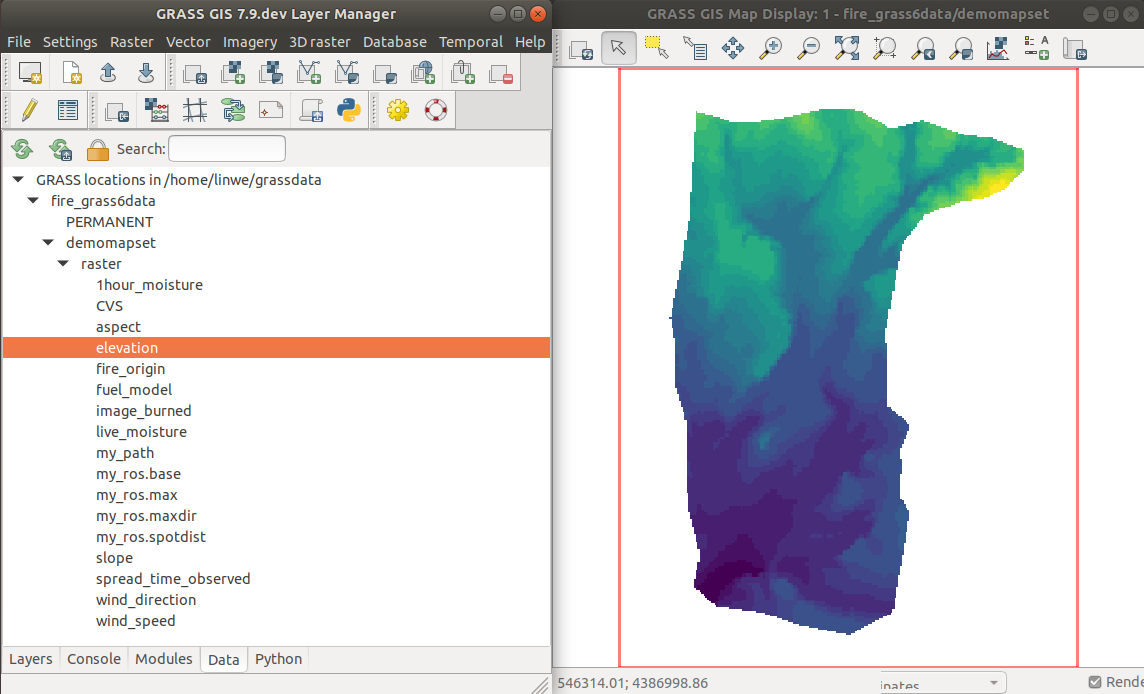
\includegraphics[width=15cm]{../pictures/data_catalog_pred.png} 
\caption[Data Catalog in Data tab (version before GSoC)]{Data Catalog in Data tab in the version before GSoC (source: own)}
\label{fig:data_catalog_pred}
\end{center}
\end{figure}



\newpage
\vspace*{-1cm}
\subsubsection{Startup mechanism}
\label{section:mechanism}
\noindent
\large
This work talks about the startup mechanism, which is a concept that was introduced directly for the purposes of this work. No publications working with this term could be found. This is probably due to the facts that many software programs are developed commercially and most commonly used software or applications do not require any more complex initial setup. However, this is not the case here. It is therefore necessary to define what we consider by the term \textit{startup mechanism}.

\noindent The startup mechanism basically includes three things:

\begin {itemize}

\item the way the software can be started. In the case of GRASS GIS running under a Unix operating system, it is run from the command line.

\item components that the user encounters during startup. In the case of GRASS GIS version 7.8, these are the Startup screen, Location Wizard and Splash Screen. There may be situations where the requested mapset is locked (this happens if it is used by another process, or if the last session in this mapset ended in an error). If the running mapset is locked, we will be notified first after starting the Session that there is a lock file with a .gislock extension in the mapset, and then asked if we want to delete this file. In this special situation, when running GRASS, we even encounter five different components.
In the case of the version after GSoC, the mentioned components are bypassed in most situations and we can move straight to the third point.

\item software state after startup (here we can talk about the state of individual Layer Manager tabs, or whether there is something shown in the Map window immediately after starting GRASS). From the point of view of the Layer Manager, the Data tab (and subsequently the Data Catalog contained in it) will be the most important for us, as it is related to the organization of work in GRASS GIS. Correct and understandable setting of the data hierarchy is an important goal of the startup mechanism.

\end{itemize}

\newpage
\vspace*{-1cm}
\subsection{Usability testing methods}

\noindent As Ana Amélia describes in her work [], the concept of usability is related to the field of Human-Computer-Interaction (HCI). Here we can find several definitions of what usability means. In the case of websites and software applications, usability refers to whether or not users can achieve specific goals with efficiency, effectiveness and satisfaction (Marcie Dishman). Booth (1989) mentions four aspects of usability testing: usefulness, effectinevess (ease fo use), learnability, and attitude.

As explained by https://www.hotjar.com/usability-testing/methods/, the main goal of usability testing is to test and validate the product hypothesis and specific design decisions using the end-user perspective. We can come across various options for dividing usability testing methods. The most recently used distribution, for example, at https://www.hotjar.com/usability-testing/methods/, https://usabilitygeek.com/remote-usability-testing-best-practices/ is as follows:

\begin{itemize}
\item	Moderated vs. unmoderated
\item	Remote vs. in person
\item	Explorative vs. assessment vs. comparative
\end{itemize}

\noindent A moderated testing is done with direct supervision. It investigates the reasoning behind user behaviour which allows a researcher to dig deeper into any pain points and usability issues. To test participants, answer their queries, and ask follow-up questions takes about 1 – 2 hours, and average number of participant is 3 – 5 (https://www.playbookux.com/10-popular-usability-testing-methods/). 

Conversely, an unmoderated test is not supervised. The participant is usually in their own home using their own devices to test the software usability. The problem is that an average tester might not understand the complexities of a product which can consequently cause the testing in a different way than was originally intended. It takes about 20 minutes and average number of participant is 5- 10 (https://www.playbookux.com/10-popular-usability-testing-methods/).

In-person testing provides very valuable data since researchers can also watch and analyze participants’ emotions. 
Remote testing are done over the internet or by phone and doesn’t go as deep into a participant’s reasoning. However, it allows a research to test large numbers of people in different geographical areas using fewer resources.

\noindent Explorative tests are open-ended, participant are asked to give opinions, think about new features. Assessment research tests a user's interaction with the product and how well they are able to use it.  It's used to evaluate the product's general functionality. Comparative research methods involve asking users to choose which of two solutions they would prefer.

\noindent User testing methods are very nicely captured on the following picture \ref{fig:usability_testing_methods}:

\vspace{0.3cm}
\begin{figure}[hbt!] 
\begin{center}
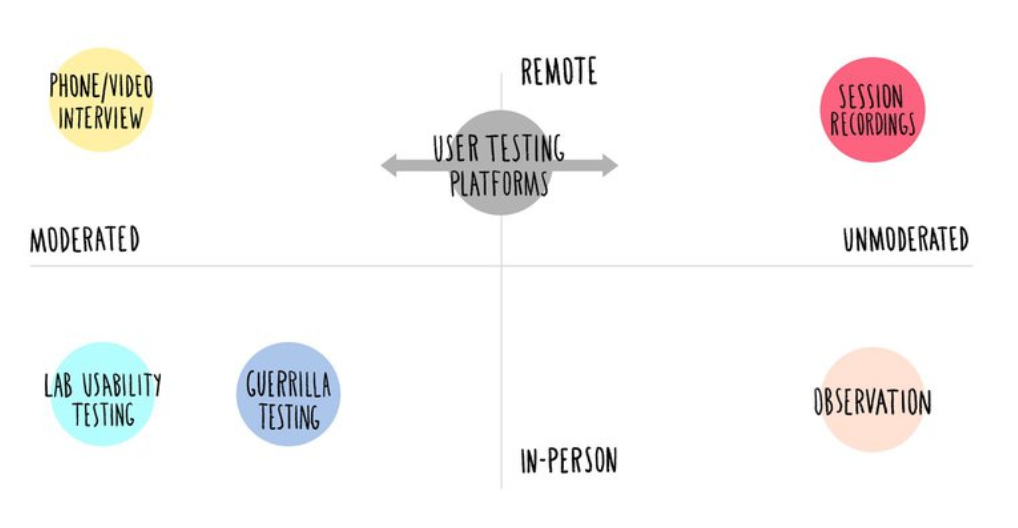
\includegraphics[width=15cm]{../pictures/usability_testing_methods.png} 
\caption[Usability testing methods]{Usability testing methods (source: https://www.hotjar.com/usability-testing/methods/)}
\label{fig:usability_testing_methods}
\end{center}
\end{figure}

\noindent It is important to emphasize that usability testing, using an appropriate method, is a valuable investment in a software product.
 
\subsubsection{Moderated + in-person usability testing}
Those tests are the best  in terms of collecting depth, comprehensive information. 
\smallskip

\noindent \textbf {Guerrilla testing}

\noindent This is the simplest form of usability test best in the early stages of the product development process. The people are asked to perform a quick usability test (maximum 10 minutes), often in exchange for a small gift. Test subjects are chosen at random from a public place, so that they may have no history with a product. This is the reason why Guerrilla testing is not suitable for testing products that require having special skills.

\smallskip

\noindent \textbf {Lab usability testing}

\noindent This type of usability research usually takes place inside the controlled environment that is different from the user’s real environment. 
Lab usability testing works best if we need very comprehensive and detailed information about how the user works with the program and what problems they encounter. Participants perform tasks and the researcher monitors them and asks questions. It is important that the moderator is trained and able to help participants, but at the same time he should let them think and not tell them exactly what to do. The moderator should also be able to read human emotions. After testing, it is also crucial to discuss and analyze the specific problems they have faced.

\subsubsection{Moderated + remote usability testing}
Moderated and remote usability tests are performed via a computer or phone and require a trained moderator. They are good for picking from a wide range of participants while still taking advantage of a moderator's skills and ability to dive deep.

\smallskip

\noindent \textbf {Phone interviews}

\noindent In a phone usability test, a moderator verbally instructs participants to complete tasks on their computer and collects feedback while the user interaction is recorded remotely. This is a very good option to test users all over the world. 

\smallskip

\noindent \textbf {Card sorting}

\noindent Card sorting is the simple method which involves placing concepts or features on virtual cards and allowing participants to manipulate the cards into groups and categories. After they sort the cards, they explain their logic to a moderator. It is used for better organizing content and features in user interface.

\subsubsection {Unmoderated + in-person}
Unmoderated in-person tests offers many of the benefits of testing in a controlled atmosphere and reduces the possibility that a researcher could influence participants with their questions.

\smallskip

\noindent \textbf {Contextual inquiry}

\noindent Sometimes also called the Interview/Observation is the method especially suitable for obtaining information about the user's habits and preferences or to evaluate whether the user is satisfied with the product. The researcher first asks a series of questions about the experience with the product and then gives the user a task to work on independently. A research will not provide any opinions and can only interfere if the participant gets stuck on something. Otherwise a observer remains silent,  focuses mainly on the emotions and behavior of the user, and writes notes which will be then summarized in a detailed test report.

\smallskip

\noindent \textbf {Eye-tracking}

\noindent This special method allows scientists to observe the movements of the user's eyes using a special device located on the monitor, and to create heatmaps (where the user most often looked). The disadvantage of this method is that it requires a lab with special equipment and software.

\subsubsection{Unmoderated + remote usability testing}

Test participants are asked to complete tasks alone in their own environment using their own devices. It does lead to the natural participant's behaviour, however, this type of testing is less detailed. As a researcher can obtain larger amount of data, they could be able to have more confidence in a decision concerning their product. The main point is that a researcher need to ensure that every test instruction is clear. Unclear tasks can cause results missing right objectives. It is suitable for validation of particular question or hypothesis, however, it is not recommended to be used as a first usability testing method since it does not go deep into user’s thinking.

\smallskip

\noindent \textbf {Session recordings}

\noindent Session recordings use software to record the actions that anonymized people take on a website/software such as mouse clicks, movement, and scrolling. It helps to understand what content/features are the most interesting for the users as well as what interaction problems users encounter while they interact with the product.
\smallskip

\noindent \textbf {Online testing tools and platforms}

\noindent There are a variety of online testing tools that allow one to remotely observe user behavior. The most commonly used online testing tools are 5-second test and unmoderated card sorting.  In 5-second test, participants have five seconds to look at a screenshot of page before they answer the question. It is an easy way how to collect qualitative data about people’s first impressions and reactions. Card sorting, described above, can also be conducted in an unmoderated and remote manner if a researcher leaves out on the opportunity for follow-up questions.

\newpage
\vspace*{-1cm}
\subsection{Questionnaires}

\noindent As the reader of this work probably realized surveys (questionnaires) were not mentioned among unmoderated + remote usability testing. The reason is that questionnaires are not usually considered as usability testing because it does not require to directly test product functionality. However, in some literature [6 usability, Ana Amélia], questionnaires are also included in usability testing methods. In Ana Amélia's work, for example, the survey includes both - interview and questionnaire techniques. The questionnaire refers to a technique that can fall under the so-called expert/heuristic method, which works with experienced people who identify problems a less experienced user might encounter. Therefore, in this work, the author eventually reserved a special chapter for questionnaires.

As [6 usability] writes, questionnaires are not as numerically grounded and precise as other forms or testing, but they can provide important feedback from user group in a short time. They can take the form of specific questions about the software and its future development. However, if we are interested in the assessment of perceived usability, we can use the widely used standard questionnaire known as the System Usability Scale (SUS). This questionnaire having 10 five-point items with alternating positive or negative tone was introduced by Brooke in 1996 [John Brooke]. The standard version is shown in Figure \ref{fig:sus}.

\vspace{0.3cm}
\begin{figure}[hbt!] 
\begin{center}
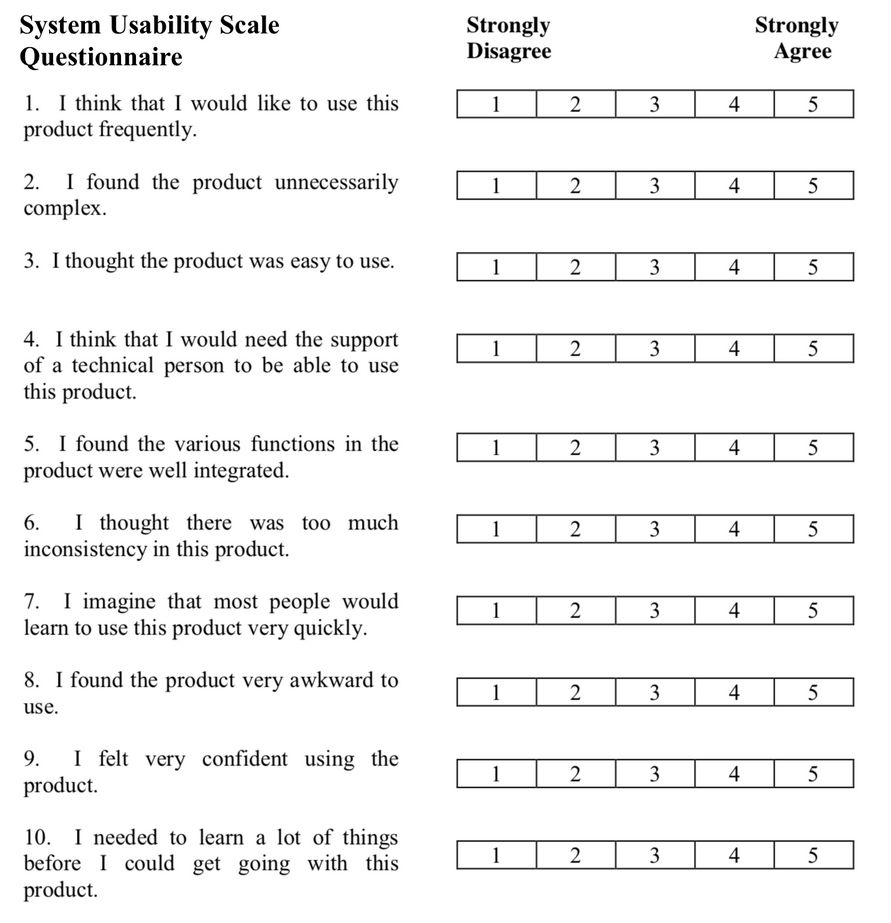
\includegraphics[width=12cm]{../pictures/sus.png} 
\caption[The Standard of the System Usability Scale (SUS) ]{The Standard of the System Usability Scale (SUS) (source: SUS - A quick and dirty usability scale John Brooke)}
\label{fig:sus}
\end{center}
\end{figure}

Questionnaires must be effective. Therefore, in this new field very different from the field of programming, it was necessary to acquire new knowledge that will help avoid beginner's mistakes. The author therefore participated in a user survey workshop within the All Things Open platform, which offers video conferencing focused primarily on improving open-source technologies. This video conference (link to a lecture) led by professionals Dan Zola and Kerry Thompson from SWAY UX set out a few key rules for creating a survey from which to get as much information as possible.

According to the lecturers, the user survey helps with evaluation of customer safisfaction as well as understanding who are users and what are their pain points and priorities. It can be conducted not only at the start of the new project but basically at any time the survey administrator (developer) needs user input.

In order to understand what makes up good questionnarre, it is first necessary to clarify what constitutes bad questionnarre. The workshop summarized the following 8 errors in particular:

\begin{itemize}
\item Too many questions (max 10 questions)
\item Convoluted questions
\item Answer choices that do not correspond with user's reasoning
\item Question that require long and comprehensive answers (if open-ended questions, always put them at the beginning)
\item Answers that could have more than one meaning
\item Answers that do not provide any information
\item Straight line answers
\item Vague answers (scale from 1-10, where an answer is 5)
\end{itemize}

The latter vague answers can occur in the case of answers with a rating scale. Although the authors of the workshop do not explicitly mention the SUS questionnaire, they strongly recommend avoiding the rating scale. The result could look similar to the following example \ref{fig:blur_scale}. It is much more advantageous to use either binary answers (Yes / No) or rank specific features / factors. Another interesting option is to use a stripe instead of a rating scale. As Matevž Pesek, Alja Isakovic concluded the stripe interface increases the intuitiveness, simplicity and speed of answering the question. Survey Monkey offers this functionality under the term Slider. In the created surveys, it was used several times together with the idea that in SUS, the user do not evaluate questions, but statements. It often happens that the user would not use the queried functionality, but they assume that the others do, which results in a positive answer. Statements encourage the user to better express their own opinions.

\vspace{0.3cm}
\begin{figure}[hbt!] 
\begin{center}
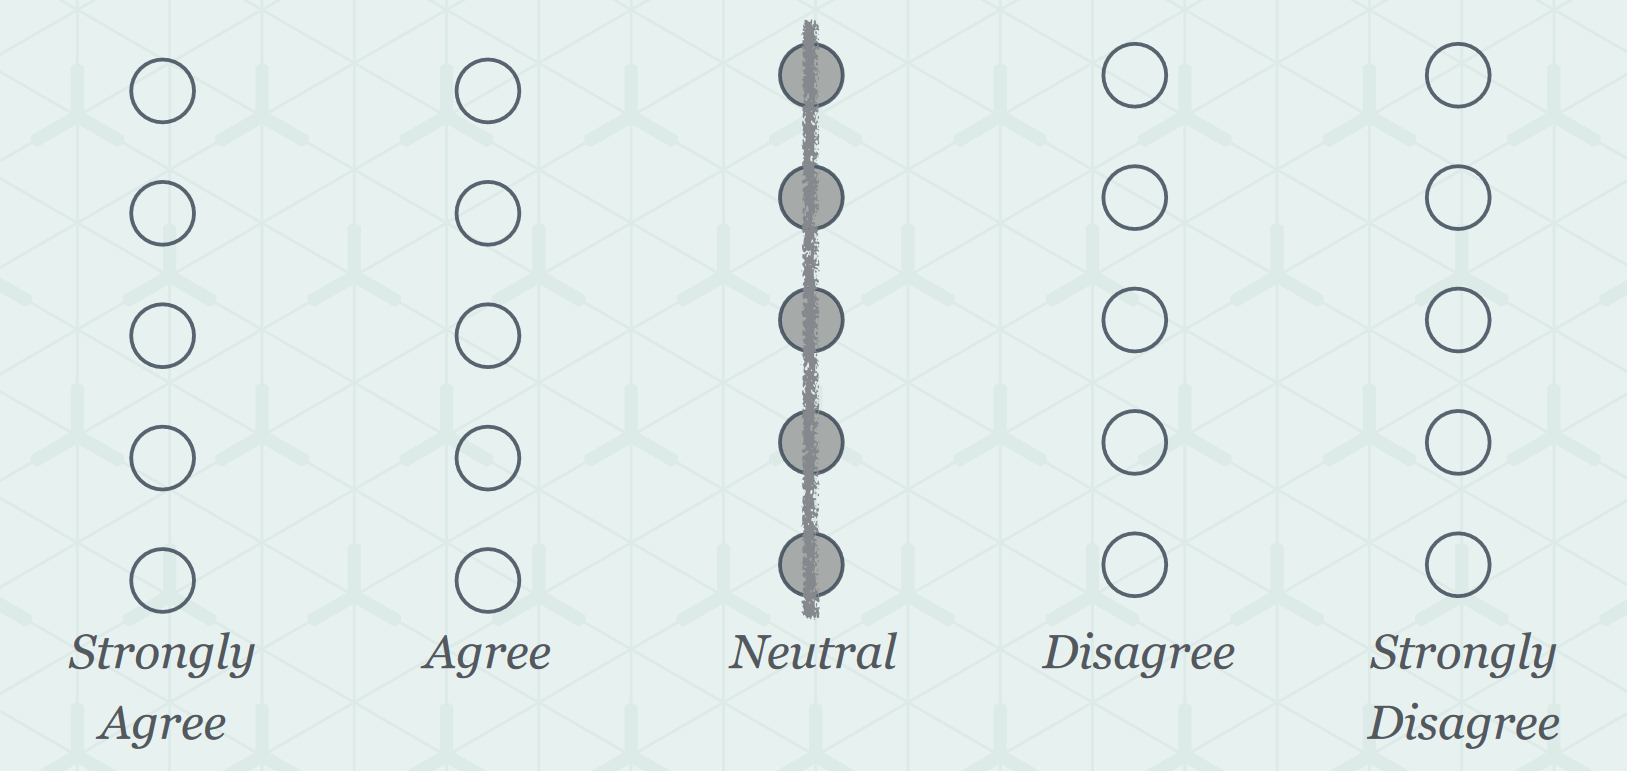
\includegraphics[width=12cm]{../pictures/blur_scale.png} 
\caption[Difficult to interpret result of the rating scale answers]{Difficult to interpret result of the rating scale answers (source: danzolakerrythompson)}
\label{fig:blur_scale}
\end{center}
\end{figure}

\noindent If we use one of the specialized platforms such as Survey Monkey or Survey Gizmo, we will be able to set different types of answers. The list offered by the Survey Monkey platform can be seen in Figure \ref{fig:survey_monkey_options}. The advantage of these tools is also that they automatically organize the answers into graphs and charts.

\vspace{0.3cm}
\begin{figure}[hbt!] 
\begin{center}
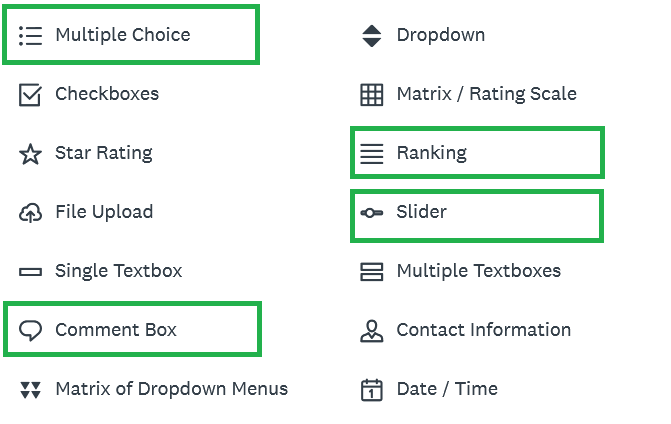
\includegraphics[width=9cm]{../pictures/survey_monkey_options.png} 
\caption[Survey Monkey answer types ]{Survey Monkey answer types (source: https://www.surveymonkey.com)}
\label{fig:survey_monkey_options}
\end{center}
\end{figure}

\noindent As mentioned at the beginning of the chapter, questionnaires are not usually considered as usability testing because it does not require to test product functionality.
However, it would be very challenging (if not impossible) in our work to ensure users having both versions of GRASS GIS (version 7.8 and version 7.9 after GSoC). Therefore, it was finally decided to use questionnaires as the main testing method.

\newpage
\vspace*{-1cm}
\fancyhead[RE, RO]{\fancyplain{}{\small \sl{State of Art}}}
\section{State of Art}
\label{State of Art}
\noindent
\large
The data hierarchy described in the previous section \ref{subsection:hierarchy} proves its worth especially when used by experienced users of GRASS, however, for complete beginners, it is rather confusing. Especially if the above-mentioned main components (database, location, and mapset) have to be defined right at the start of the software when launching the startup screen, which has been standard since version 6.4. 

Therefore, the general question was whether to keep data hierarchy at all or change the whole concept and use only \textit{project} and \textit{map} terms, which is the usual standard for other GIS software. The \texttt {database/location/mapset} mechanism may indeed seem complicated at first glance, but we must keep in mind that many later problems will be avoided by clearly defining the coordinate system at the beginning and allowing only one coordinate system within one location. From author’s point of view, the advantage (perhaps from the point of view of other users maybe the disadvantage) is that GRASS GIS does not support On the fly transformation. This may seem a bit rough at first, but it guarantees that we will not analyze data having a different coordinate system together, as could happen in ArcGIS or QGIS, for example. In these software, it can be confusing to see differently designed data in the right place on the map. In GRASS GIS, we also cannot get into a situation that the On the fly transformation does not occur at all, but even so it is allowed to display two layers of different coordinate systems on top of each other. This, of course, results in incorrect rendering of the layers in the map window (may happen e.g. in SAGA GIS).

Considering the disadvantages mentioned above, it seems very unfortunate to disrupt this system. Rather, it is important to clearly introduce it to newcomers. In the startup screen of version 7.8 (state before GSoC) there is a certain effort to provide the first-time user with the maximum possible help (short description of data hieararchy, Help button), but even so, the development community often encountered misunderstanding from the ranks of users \footnote{\url{https://trac.osgeo.org/grass/ticket/3474}}. 

Therefore, in 2017, the first suggestions on how to simplify this startup screen began to appear. In terms of implementation complexity, the simplest and most effective proposal seemed to be the A3 proposal. In Prague in 2019 an implementation proposal, also known as the Prague Roadmap\footnote{\url{https://trac.osgeo.org/grass/wiki/wxGUIDevelopment /New\ _Startup\#PragueRoadmap}}.  was created based on A3. A brief summary of the proposed implementation is contained in the next subchapter.

\newpage
\vspace*{-1cm}
\subsection{Prague Roadmap}
\label{section:Prague Roadmap}

The most serious changes concern the Data Catalog. They lie in supporting multiple databases, adding buttons to create existing or new databases, or adding new actions from the context menu to a database, location, and mapset node. The data hierarchy \texttt{database/location/mapset} is preserved and in addition, this proposal introduces a new concept called Workspaces which is not directly part of the Mapset, but is associated with it.

The same Data Catalog implemented in the Data tab is then planned to be used within startup screen inspired by A2 proposal designed by Garrett Millar. However, unlike the A2 design, the startup screen has no other tabs. It consists of only one startup page, which has a Data Datalog in the center, and a toolbar with big buttons for creating or defining new or existing hierarchy components, such as a location or mapset.

The proposed changes in the Location Wizard are mainly related to the clarification of the first page, better naming of the given attributes and speeding up the selection of the coordinate system in the dialog.

Furthermore, the proposal assumes the possibility of filtering in the Data Catalog based on the recently selected items. General startup GUI should be able to collect recent maps and workspaces as well as used databases and workspaces. The display of map layers in the Data Catalog is switched off by default, the display of workspaces under the relevant mapset is switched on. When GRASS GIS launches, a "grassdata" directory for storing locations, mapsets and maps should be automatically created in a reasonable place.


\subsection{Version 7.9 after Google Summer of Code}
\label{subsection:Version 7.9 after Google Summer of Code}
\noindent
The first part of this work focuses on a survey among intermediate users. One of the goals of this survey is to let users evaluate the changes in the version 7.9 after GSoC. Therefore, it is necessary to describe in detail what improvements Google Summer of Code has brought and in what is the appearance of the software at the time of the first survey.
Since the startup mechanism includes more or less interconnected software components that the first-time as well as experienced user will encounter almost one hundred percent at startup, the following subchapter is further divided into several smaller subsections. This time the software components are ranked according to their importance in version 7.9 after GSoC.


\newpage
\vspace*{-1cm}
\subsubsection{Data Catalog}

The main goal of GSoC was to improve the Data Catalog in such a way which enables a user-friendly organization of work. One may argue that these improvements are not related to the startup mechanism, but the truth is that the current version of the Data Catalog takes over the role of startup screen, and even offers more functionality. In the Figure \ref{fig:function} we can see the functions that have been newly implemented in the Data Catalog.

\vspace{0.3cm}
\begin{figure}[hbt!] 
\begin{center}
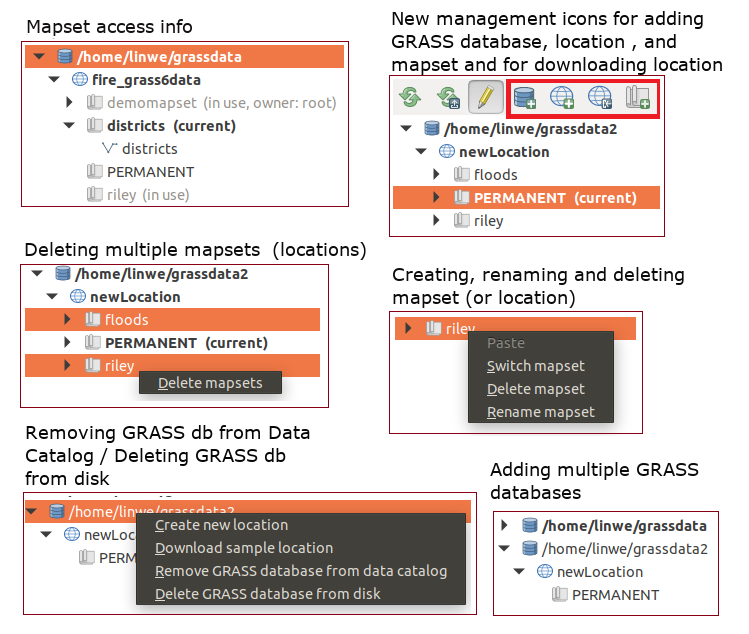
\includegraphics[width=15cm]{../pictures/funkce.png} 
\caption[New functionalities in Data Catalog ]{New functionalities in Data Catalog (source: own)}
\label{fig:function}
\end{center}
\end{figure}

\noindent This is mainly about creating, renaming and deleting mapsets and locations, which was previously possible through the startup screen. However, completely new possibilities have been added. GRASS GIS allows you to add multiple databases. New management icons offer intuitive creation of the mentioned data components. In the context menu there are also new options for deleting several mapsets or locations.

\newpage Though, probably the most visible changes are those related to the graphical representation of the Data Catalog. Next to the individual components, we can notice small icons distinguishing which component of the data hierarchy it is. The Data Catalog also informs about access to individual mapsets (current, in use, and a different owner).

Another important thing is related to access to individual mapsets. In version 7.8, the startup screen informs about the lock and asks if the user wants to remove the lock.
In order to completely take over the startup screen functionality by the Data Catalog, it is also necessary to warn the user that the mapset to which they are going to switch is locked. How this case was solved is clear from the Figure \ref{fig:data_catalog_switch_new}. Because mapset locking was often confused with prohibiting editing outside the current mapset, the term was changed to \textit{mapset in use}. This term can also be seen in the Mapset Access Info in the Data Catalog.

\vspace{0.3cm}
\begin{figure}[hbt!] 
\begin{center}
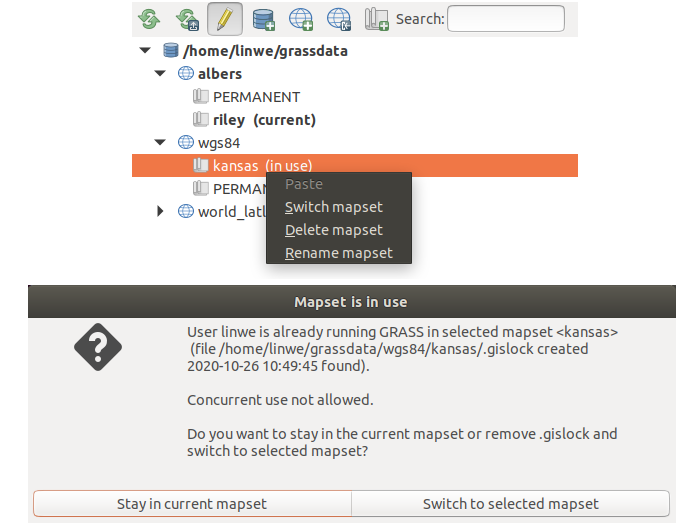
\includegraphics[width=12cm]{../pictures/data_catalog_switch.png} 
\caption[Switching to mapset in use in Data Catalog]{Switching to mapset in use in Data Catalog (source: own)}
\label{fig:data_catalog_switch_new}
\end{center}
\end{figure}

\noindent Another important step forward was the graphic change of the icon enabling or disabling changes outside the current mapset. Now this icon has the character of a pencil (similar to QGIS) and protects us from unwanted changes. If we do not have editing enabled, we cannot rename or delete any mapsets, locations and databases. We can only work with layers inside the current mapset. However, even if we enable editing, we can never delete a PERMANENT mapset. Similarly, we cannot delete boldly marked ``current” components in the Data Catalog.

\newpage
\vspace*{-1cm}
\subsubsection{Location Wizard}

This guide to creating new locations has been slightly modified and streamlined. In particular, we can see it on the first page ``Define a new GRASS location'' in Figure \ref{fig:loc_wiz_1}. Checkboxes and simplified names are removed here. The GRASS database can be newly modified.

\vspace{0.3cm}
\begin{figure}[hbt!] 
\begin{center}
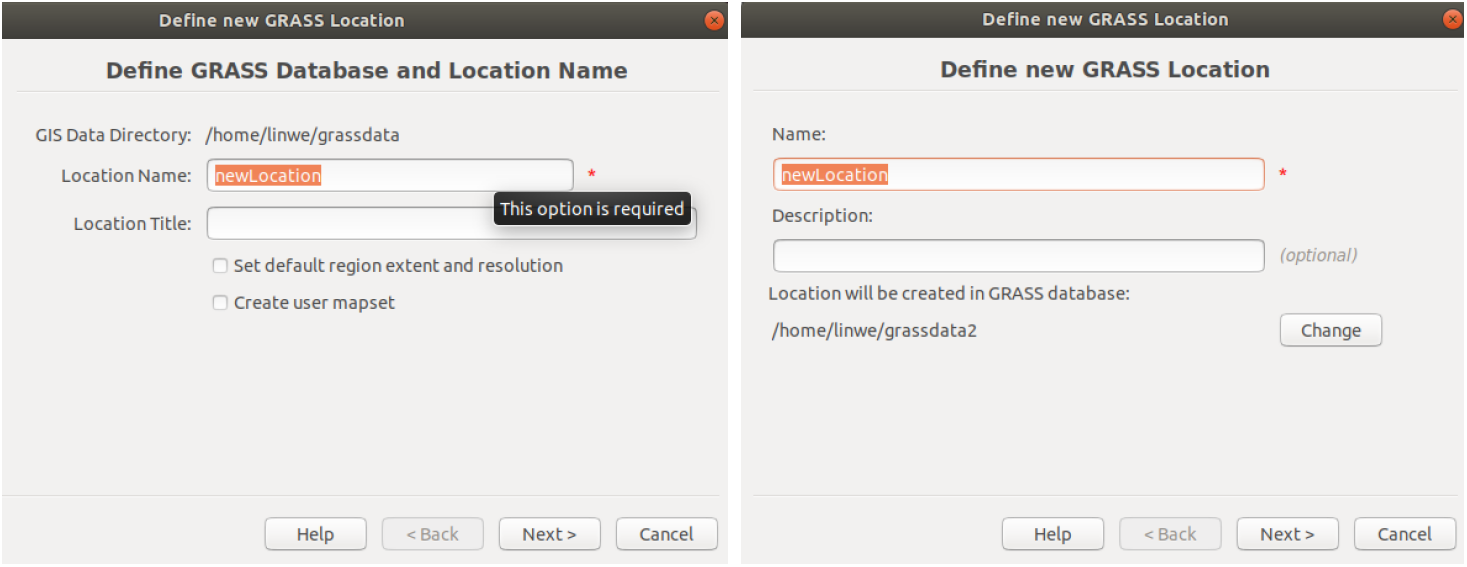
\includegraphics[width=15cm]{../pictures/loc_wiz_1.png} 
\caption[Location Wizard first page before and after GSoC]{Location Wizard first page before and after GSoC (source: own)}
\label{fig:loc_wiz_1}
\end{center}
\end{figure}

\noindent The second page is renamed to ``Select Coordinate Reference System (CRS)''. As we can see in Figure \ref{fig:loc_wiz_2}, in the original version there is a division into simple and advanced methods, which is abolished in the new version. In addition, CRS can be newly specified using a WKT string.

\vspace{0.3cm}
\begin{figure}[hbt!] 
\begin{center}
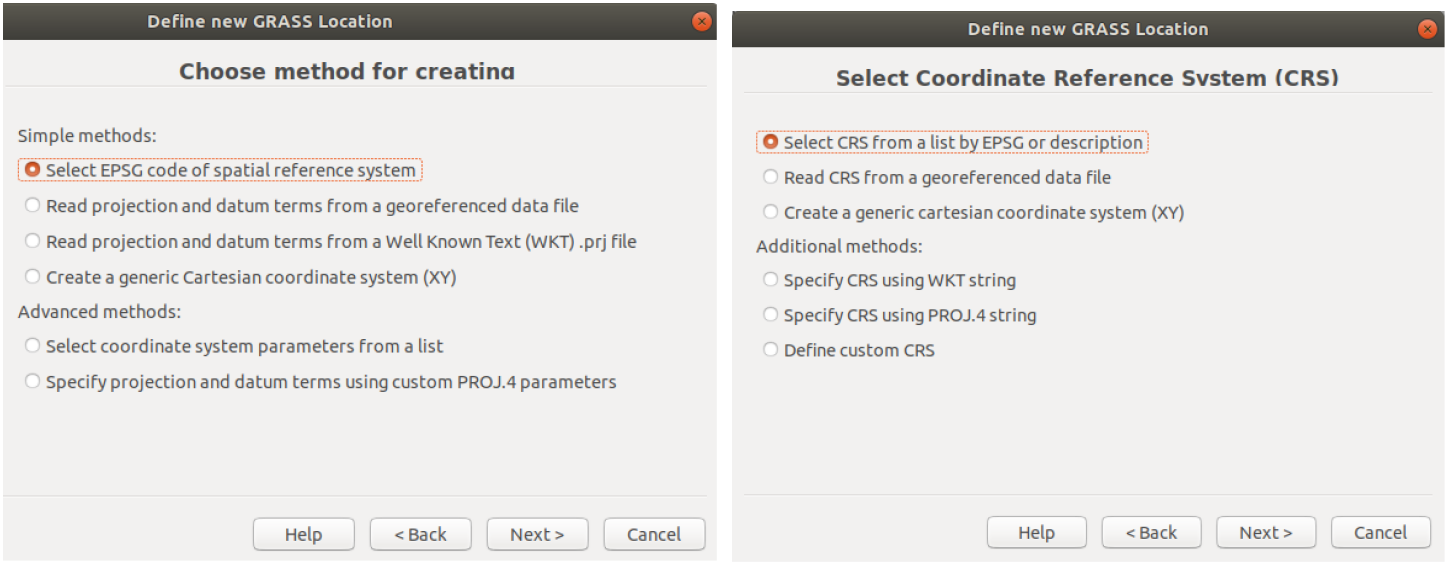
\includegraphics[width=15cm]{../pictures/loc_wiz_2.png} 
\caption[Location Wizard second page before and after GSoC]{Location Wizard second page before and after GSoC (source: own)}
\label{fig:loc_wiz_2}
\end{center}
\end{figure}

\newpage
However, the essential change is related to ``Choose EPSG code'' page. Now it supports dynamic EPSG search. Furthermore, it provides the hyperlink to EPSG pages which is being changed dynamically according to a filter set by a user (see Fig. \ref{fig:loc_wiz_3}). The last page of the Location Wizard called ``Summary'' remains unchanged.


\vspace{0.3cm}
\begin{figure}[hbt!] 
\begin{center}
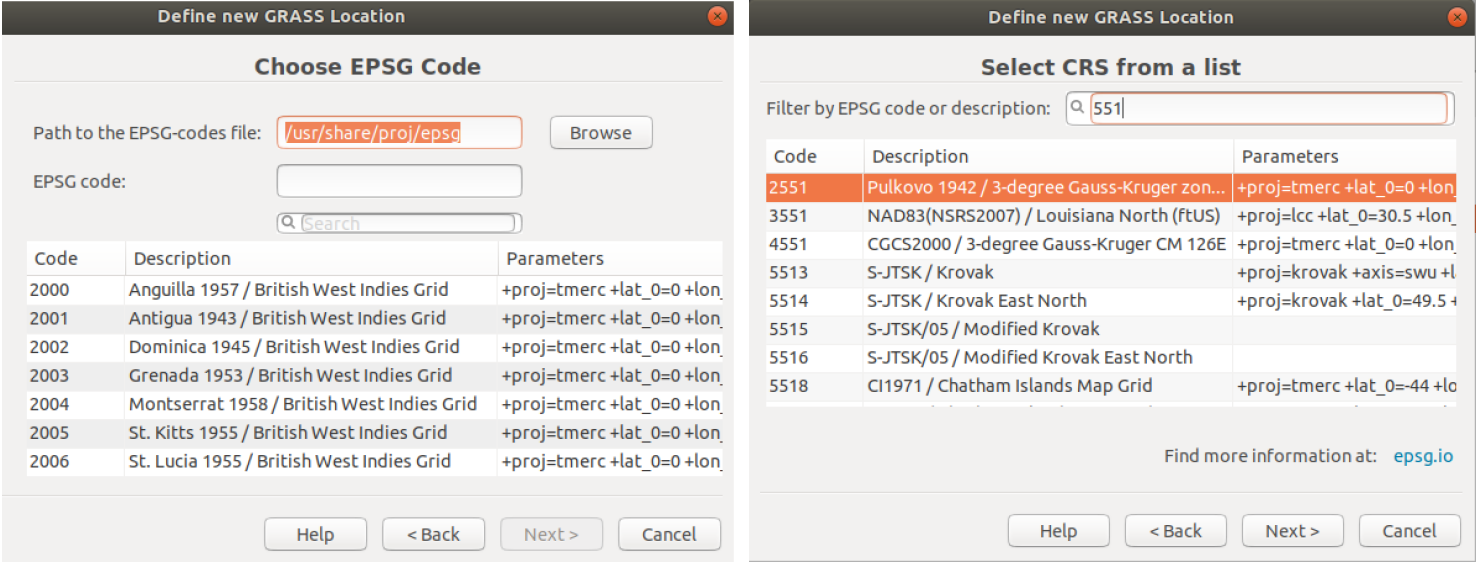
\includegraphics[width=15cm]{../pictures/loc_wiz_3.png} 
\caption[Location Wizard third page before and after GSoC)]{Location Wizard third page before and after GSoC (source: own)}
\label{fig:loc_wiz_3}
\end{center}
\end{figure}


\subsubsection{Startup screen}

The changes that occurred during the Google Summer of Code were fundamental. At first, it was definitely not planned to remove the startup screen. The changes were to be based on Proposal A3, which planned to improve the Data Catalog, but also suggested that the same Data Catalog, which is available in the Data tab after starting the session, will be part of the startup screen.
During the implementation, however, all the functionality of the startup screen, including switching mapsets as well as locations and databases, was moved to the Data Catalog, so it no longer made sense to keep this notion. At least definitely not the form in which it is in the version 7.8.

\noindent We can encounter three different situations when starting the GRASS GIS development version:

\begin{enumerate}

\item GRASS is launched directly with the Data Catalog visible in the prepared Demolocation (see Figure \ref{fig:demolocation_startup}). This situation occurs after the software is installed, that is, when no used databases are stored in the settings. Demolocation called /textit{world\_latlong\_wgs84} shows the correct organization of the data. Original data are stored in a permanent mapset whereas already analyzed data belongs to another mapset, for example to the one named after a user. The current implementation does not show a world map immediately at startup, it is necessary to display the map using Data Catalog (see Fig. \ref{fig:demolocation}).

\vspace{0.3cm}
\begin{figure}[hbt!] 
\begin{center}
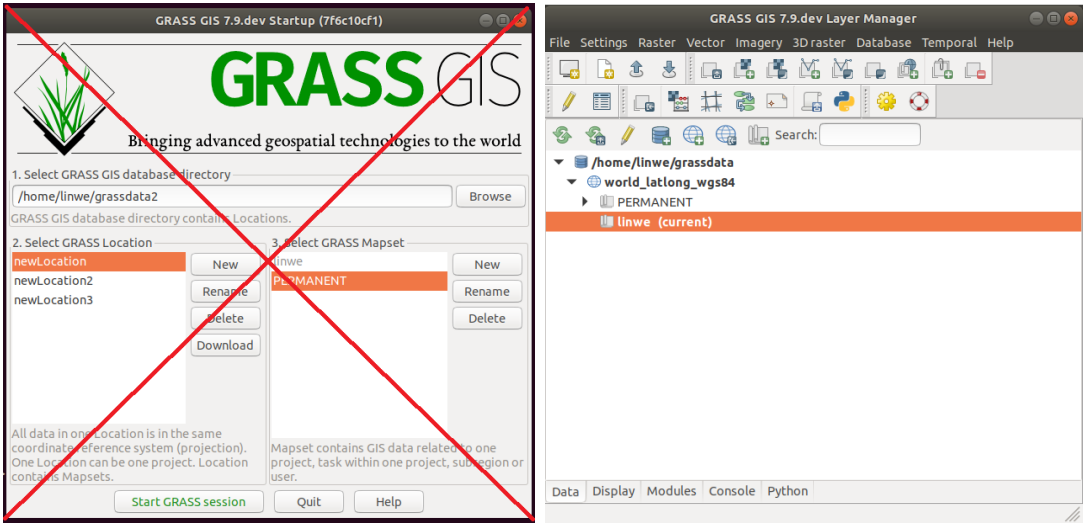
\includegraphics[width=15cm]{../pictures/demolocation_startup.png} 
\caption[GRASS launched with the Data Catalog in the prepared Demolocation]{GRASS launched with the Data Catalog in the prepared Demolocation (source: own)}
\label{fig:demolocation_startup}
\end{center}
\end{figure}

\vspace{0.3cm}
\begin{figure}[hbt!] 
\begin{center}
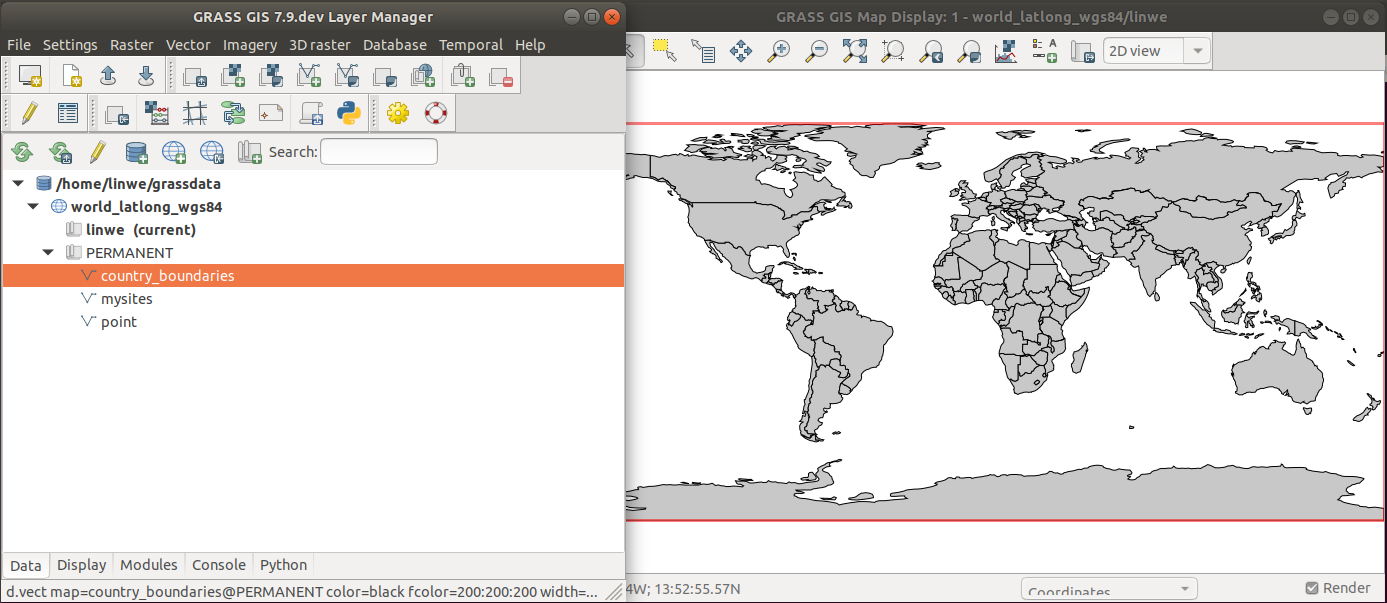
\includegraphics[width=15cm]{../pictures/demolocation.png} 
\caption[World map as a part of Demolocation]{World map as a part of Demolocation (source: own)}
\label{fig:demolocation}
\end{center}
\end{figure}

\item GRASS bypasses the Startup screen if possible to start in the last used mapset (see Figure \ref{fig:last_mapset_startup}). This situation is probably the most common. The software remembers the databases that were open when the last session was closed and opens them.

\vspace{0.3cm}
\begin{figure}[hbt!] 
\begin{center}
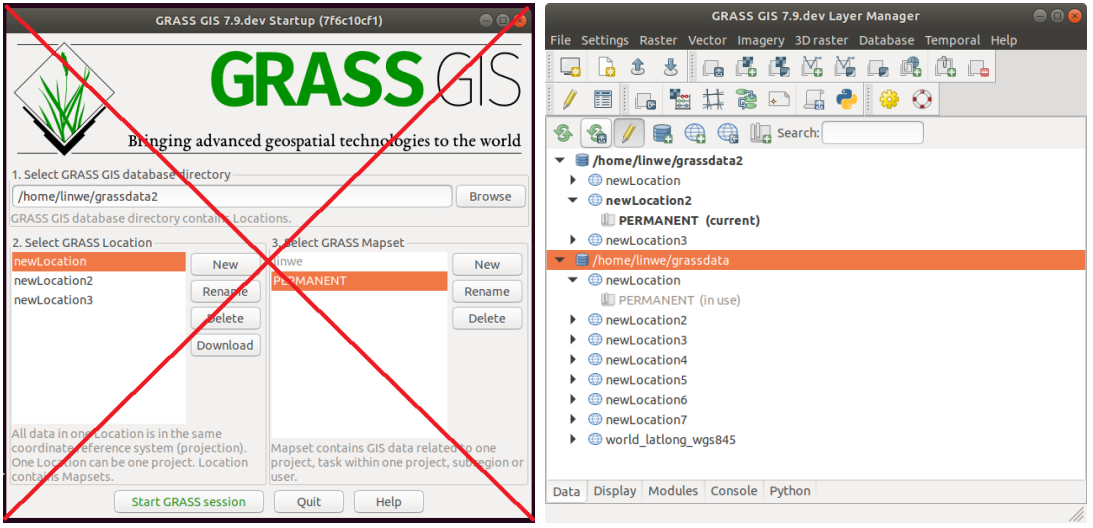
\includegraphics[width=15cm]{../pictures/last_mapset_startup.png} 
\caption[Data Catalog in Data tab (version before GSoC)]{Data Catalog in Data tab in the version before GSoC (source: own)}
\label{fig:last_mapset_startup}
\end{center}
\end{figure}

\newpage
\item GRASS GIS launches in Startup screen if a mapset is not in a usable state (was deleted or is used by another process). In this special situation, GRASS starts in the same way as in the version 7.8.

\end{enumerate}

\subsubsection{Various options for starting GRASS}

\large \noindent In addition to the software components that the user encounters during startup and to the state that the software finds itself immediately after startup, the startup mechanism also includes the way we run the software. Because users of this software usually work under a Unix operating system, GRASS GIS is usually run from the command line. Advanced users often do not even run the graphical environment and perform all geographic analyzes using the command line. This is also why the command line window runs in the background throughout the work with this software. In our work, however, we mainly focus on first-time users who do not have to be experienced. This is also basically the main reason why we try to improve GRASS GUI.

 \noindent To summarize, the software could be run from the command line in four ways:

\noindent \texttt{:$\sim$\$ grass79} \\
\noindent Start GRASS using the default user interface. In the version 7.8, the user is prompted by the startup screen. After GSoC startup screen appears only when the mapset is not in the usable state.

\noindent \texttt{:$\sim$\$ grass79 --gui}\\
\noindent Start GRASS using the graphical user interface.  In the version 7.8, the user is prompted by the startup screen. After GSoC startup screen appears only when the mapset is not in the usable state.

\noindent \texttt{:$\sim$\$ grass79 --text} \\
\noindent Start GRASS using the text-based user interface. Appropriate location and mapset must be either set by environmental variables or taken from the last GRASS session.

\noindent \texttt{:$\sim$\$ grass79 --gtext} \\
\noindent Start GRASS using the text-based user interface.  In the version 7.8, this option as the only one does not display the Startup screen. However, it means that desired location and mapset must already be set as environmental variables, for example by running a specific mapset using the \texttt{:$\sim$\$ grass78 \$HOME/grassdata/location/mapset} command, or taken from the last GRASS session, specifically from a file in the path \textit{\$HOME/.grass7/rc}, which stores the current mapset and current location when the software is closed.
In the version 7.9, --gtext uses startup screen but then does not run the GUI.

There are two other topics related in part to starting the software. The first is the splash screen. In the new implementation, the splash screen does not appear during normal startup. The second thing that could further expand the possibilities of starting GRASS is the new concept of Workspaces. In the development version of the software version, it is possible to save the current software settings and then open it, as we can see in Fig. \ref {fig:workspace_grass}. However, there is no option to start a specific workspace from the command line or to start GRASS GIS from File Manager using the file association of the workspace file (.gxw).

\vspace{0.3cm}
\begin{figure}[hbt!] 
\begin{center}
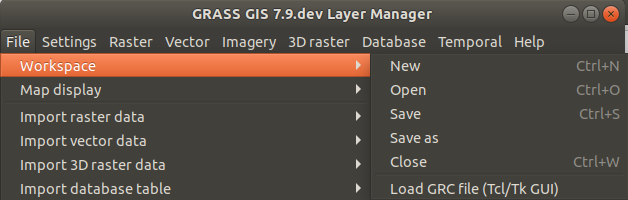
\includegraphics[width=13cm]{../pictures/workspace_grass.png} 
\caption[Management of Workspaces in the Layer Manager]{Management of Workspaces in the Layer Manager (source: own)}
\label{fig:workspace_grass}
\end{center}
\end{figure}


\newpage
\vspace*{-1cm}
\subsection{Suggestions for improvement}

After GSoC, two fundamental questions arose, to which we will try to find answers in this work:

\begin{enumerate}

\item  \noindent \textbf{Would be implementing a special mode for first-time user helpful? What should this first-time mode look like?}

\noindent As mentioned at the beginning of this chapter, data hierarchy in GRASS GIS can cause significant problems for newcomers. Therefore, the core question of this work is how to enhance the first-time user experience.

\item \noindent \textbf{How to start GRASS in a special situation when the last opened mapset is not in the usable state?}

As mentioned in the previous chapter, in the special situation where the last opened mapset is not in the usable state (is in use or was deleted), the ``old'' startup screen still appears. This situation is rather a lack of a new solution and one of the goals of this work is to eliminate this shortcoming. 

\end{enumerate}

\noindent Other questions can be:

\begin{enumerate}
\setcounter{enumi}{2}

 \item \noindent Should the world map automatically appear in the Map Display when Demolocation starts?
 
 \item \noindent What other functions to add to the Data Catalog?
 
  \item \noindent Does it make sense to add a file association of the workspace file (.gxw) in order to be able to start GRASS GIS from File Manager?
  
 \item \noindent How to solve starting with the command \texttt{:$\sim$\$ grass78 --gtext}? Cancel or keep and run g.gui.datacatalog instead of the old startup screen?
 
 \item \noindent Show splash screen when starting software?
\end{enumerate}

\noindent The aim of this work is to find answers to the above questions, to propose a solution and in the case of first two question also to implement it. The solution will be compiled on the basis of two different sources - according to trends in current GIS software and especially according to the results of the first two surveys among intermediate users. The first survey aims to improve the startup mechanism, while the second seeks to answer the question of how to enrich the first-time user experience in GRASS GIS. As feedback from users is very valuable, the aim of the first survey in particular is to find out, among other things, how satisfied users are with the new state after GSoC.


%% -------<<< Chapter 2: Concepts of startup mechanism >>>-------\\%%%%%%%%%%%%%%%%%%%%%%%%%%%%%%%%%%%%
\newpage
\vspace*{-1cm}
\fancyhead[RE, RO]{\fancyplain{}{\small \sl{General startup concepts}}}
\section{General startup concepts}
\label{sec:startup_concepts}
\noindent
\large
As the author already mentioned, the most commonly used software or applications usually do not require any more complex initial setup. However, this may not be the case for GIS software. Therefore, the following subsection introduces and compares several GIS approaches in terms of startup mechanisms. Then we move even beyond GIS and look especially on the way, how software programs chosen according to the first survey enhance the first-time user experience.

\subsection{GIS software}
\label{subsection:GIS software}

The startup mechanisms are analyzed from various perspectives, which are summarized in the final table identifying several questions:
\begin{itemize}
\item Does the GIS software have its own startup screen, and if so, how does it look like? 
\item Does the software have file association of project file?
\item Does the software offer first-time mode to help complete beginners, and if so, in what form?
\item How the software works with data of different coordinate systems? Does it support On the fly transformation? Does it allow the incorrect display of two layers of different coordinate systems on top of each other?
\end{itemize}

\noindent On Figures \ref{fig:hodnoceni_all} and  \ref{fig:hodnoceni_free} we can see graphs of the 10 highest rated GIS software and the 10 highest rated Free GIS software in the world in 2020, as stated in the evaluation taken by online magazine GISGeography. The evaluation of selected software is performed on a point scale from 0 to 10 in four categories - \textit{cartography, analysis, editing and data management} which are subsequently averaged. 

In the first place we can notice two representatives of ESRI - ArcGIS Pro, ArcGIS Desktop. I would also mention the other two interesting commercial software GeoMedia (Hexagon) and MapInfo Professional. If we focus only on Free GIS Software, in the first places in descending order we can find QGIS 3, QGIS 2, gVSIG, GRASS GIS, ILWIS and SAGA GIS. 

\vspace{0.3cm}
\begin{figure}[hbt!] 
\begin{center}
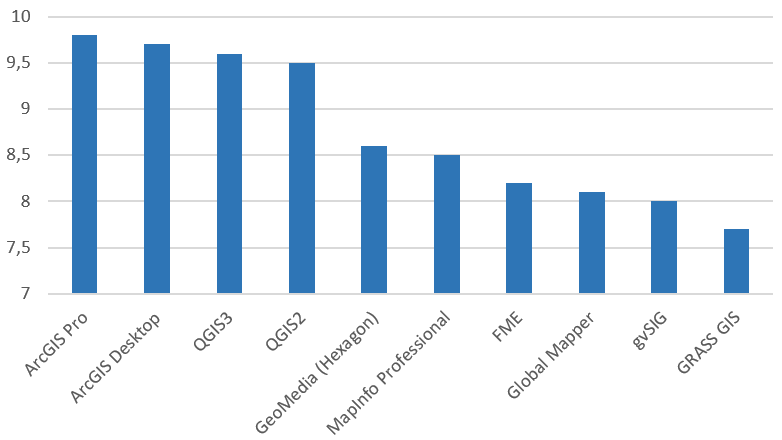
\includegraphics[width=12cm]{../pictures/hodnoceni_all.png} 
\caption[Top 10 GIS Software in 2020 according to GISGeography journal]{Top 10 GIS Software in 2020 according to GISGeography journal}
\label{fig:hodnoceni_all}
\end{center}
\end{figure}

\begin{figure}[hbt!] 
\begin{center}
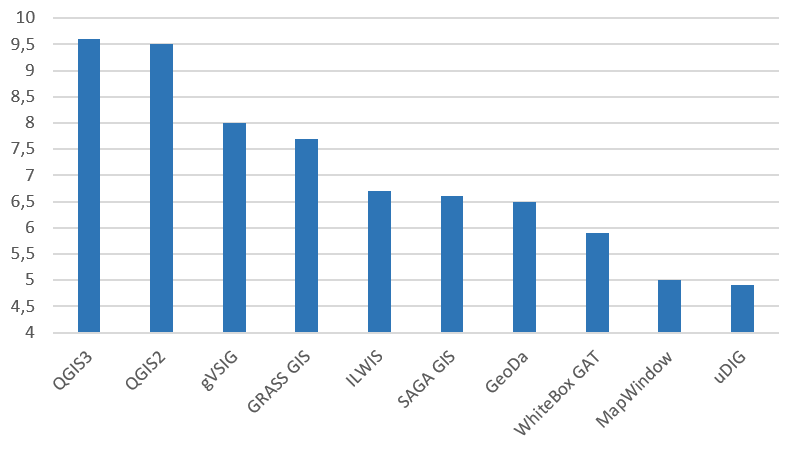
\includegraphics[width=12cm]{../pictures/hodnoceni_free.png} 
\caption[Top 10 Free GIS Software in 2020 according to GISGeography journal]{Top 10 Free GIS Software in 2020 according to GISGeography journal}
\label{fig:hodnoceni_free}
\end{center}
\end{figure}

\newpage
\noindent We must keep in mind that this evaluation is very indicative, as each software has different strengths. For example, on Figure \ref{fig:hodnoceni_analysis} GRASS GIS takes the leading position in then \textit{analysis} category, with a rating of 9.8 out of 10, which is comparable to FME and ArcGIS Pro. Among Free GIS Software GRASS has the highest rating in this aspect. This uniqueness is also mentioned in the pros of the software, which offers more than 350 geoprocessing modules, LiDAR and network analysis, sophisticated tools for satellite imagery, 3D raster rendering and customization and so forth.  The big advantage is that the GRASS GIS function can be leverage through QGIS or uDig. 

\newpage
In the disciplines of editing and data management, the balance is somewhat worse 7.4 and 7.5 out of 10 points. The biggest drop to 6.1 is in the \textit{cartography} category. At this point, however, it must be highlighted that the ambition of GRASS GIS is definitely not to create high-quality modern maps, but to offer the software for very numerically complex geographical analyzes. What is mentioned as other disadvantages is clunky and dated user interface, defining projects on start-up, steep learning curve to get started and command line window running in background. We can notice that these shortcomings are largely related to the current unfortunate startup mechanism.

\begin{figure}[hbt!] 
\begin{center}
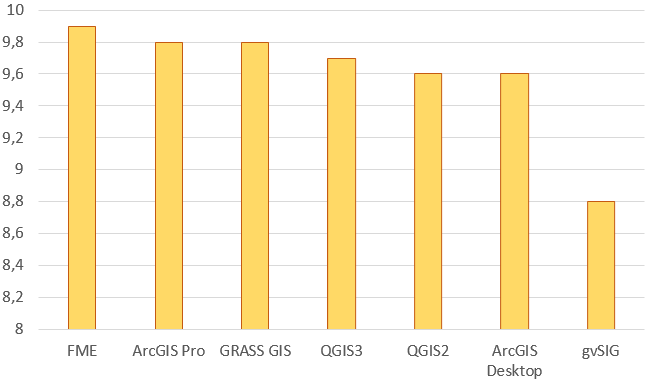
\includegraphics[width=12cm]{../pictures/hodnoceni_analysis.png} 
\caption[Top 7 GIS Software in 2020 in \textit{analysis} category according to GISGeography journal]{Top 7 GIS Software in 2020 in \textit{analysis} category according to GISGeography journal}
\label{fig:hodnoceni_analysis}
\end{center}
\end{figure}

\noindent Na tomto místě je důležité zdůraznit, že se v této práci vůbec nezaměřujeme na funkcionalitu softwarů jako takovou. Jak jste si mohli přečíst na předchozích řádcích, v tomto aspektu se softwary opravdu velmi liší. Tudíž i přesto, že daný software třeba není příliš user-friendly, konkrétnímu uživateli nezbyde než po něm sáhnout. V této práci jsou  softwary tested and analyzed in detail from the point of view of the startup mechanism and data organization with an emphasis on finding out what elements they use directly in the software to improve the first-time user experience.

Softwary jsou testovány za pomoci dvou shapefilů of different coordinate system - districts in the Czech Republic in the S-JTSK Krovak East North system (EPSG: 5514) and US tracts in the USA Contiguous Albers Equal Area Conic system  (ESRI: 102003). These systems are not selected by chance. They are defined entirely differently, however, in terms of coordinate digits they are very similar.

\newpage
\vspace*{-1cm}
\subsubsection{Analysis of selected commercial software}

\noindent On further rows three commercial representatives (ArcGIS Pro, MapInfo Professional and GeoMedia Advantage) jsou popsány z hlediska startovacích mechanismů, přívětivosti k novému uživateli a zhlediska organizace dat. U každého softwaru je vyzkoušen import dat. Autorka práce má z komerčních softwarů zkušenosti pouze s ArcMapem, se softwary ArcGIS Pro, MapInfo Professional and GeoMedia Advantage měla tu čest pracovat vůbec poprvé. Nicméně pro účely této práce je tento fakt naopak plusem, jelikož hodnocení softwarů nebude zkreslené žádnou dřívější zkušeností.

\bigskip

\noindent \textbf {ArcGIS Pro 2.4}

\noindent This software is currently the lead representative of ESRI's desktop GIS. It is an extension and connection of ArcMap, ArcScene and ArcGlobe applications. It is therefore possible to display and analyze 3D data in it.

After logging in, the startup screen is displayed (see Figure \ref{fig:arcgis_startup_screen}). Here we can open recently saved projects or select from pre-prepared templates, kterých máme na výběr hned několik - Map (standard), Catalog, Global scene and Local scene. Další variantou je vybrání empty sheet.

\vspace{0.3cm}
\begin{figure}[hbt!] 
\begin{center}
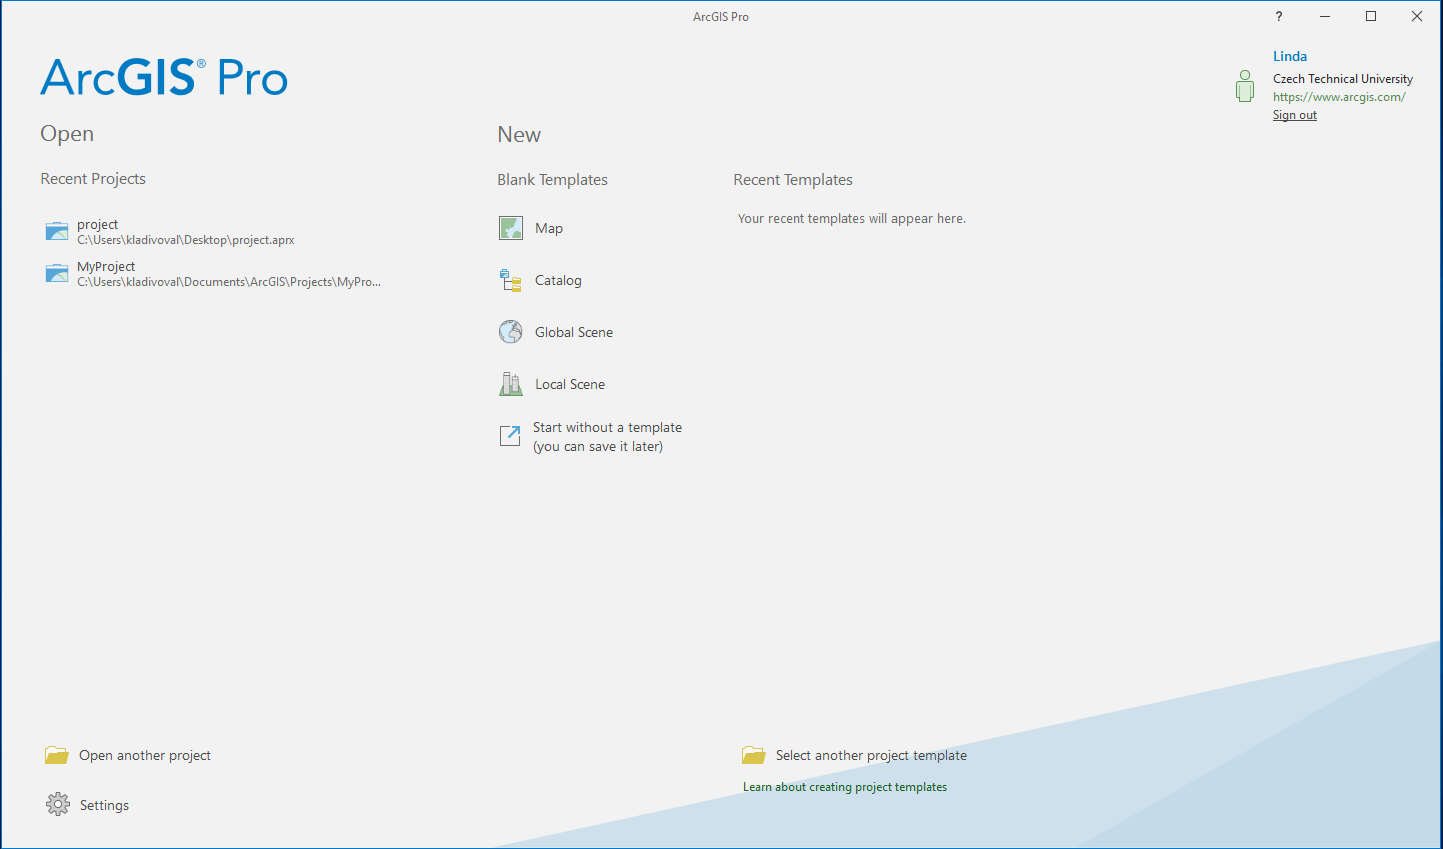
\includegraphics[width=15cm]{../pictures/arcgis_startup_screen.png} 
\caption[ArcGIS Pro 2.4 startup dialog (source own)]{ArcGIS Pro 2.4 startup dialog (source own)}
\label{fig:arcgis_startup_screen}
\end{center}
\end{figure}

\noindent The imported GIS layers are located in the Map component which is associated with Map window. In the following example on Figure \ref{fig:arcgis_pro_onthefly2}, the map window system is WGS 1984 Web Mercator Auxiliary Sphere (according to the first added layer), but the later layers added are in other coordinate systems. In spite of having different coordinate systems, the layers are displayed correctly in the map window due to On the fly transformation.

\vspace{0.3cm}
\begin{figure}[hbt!] 
\begin{center}
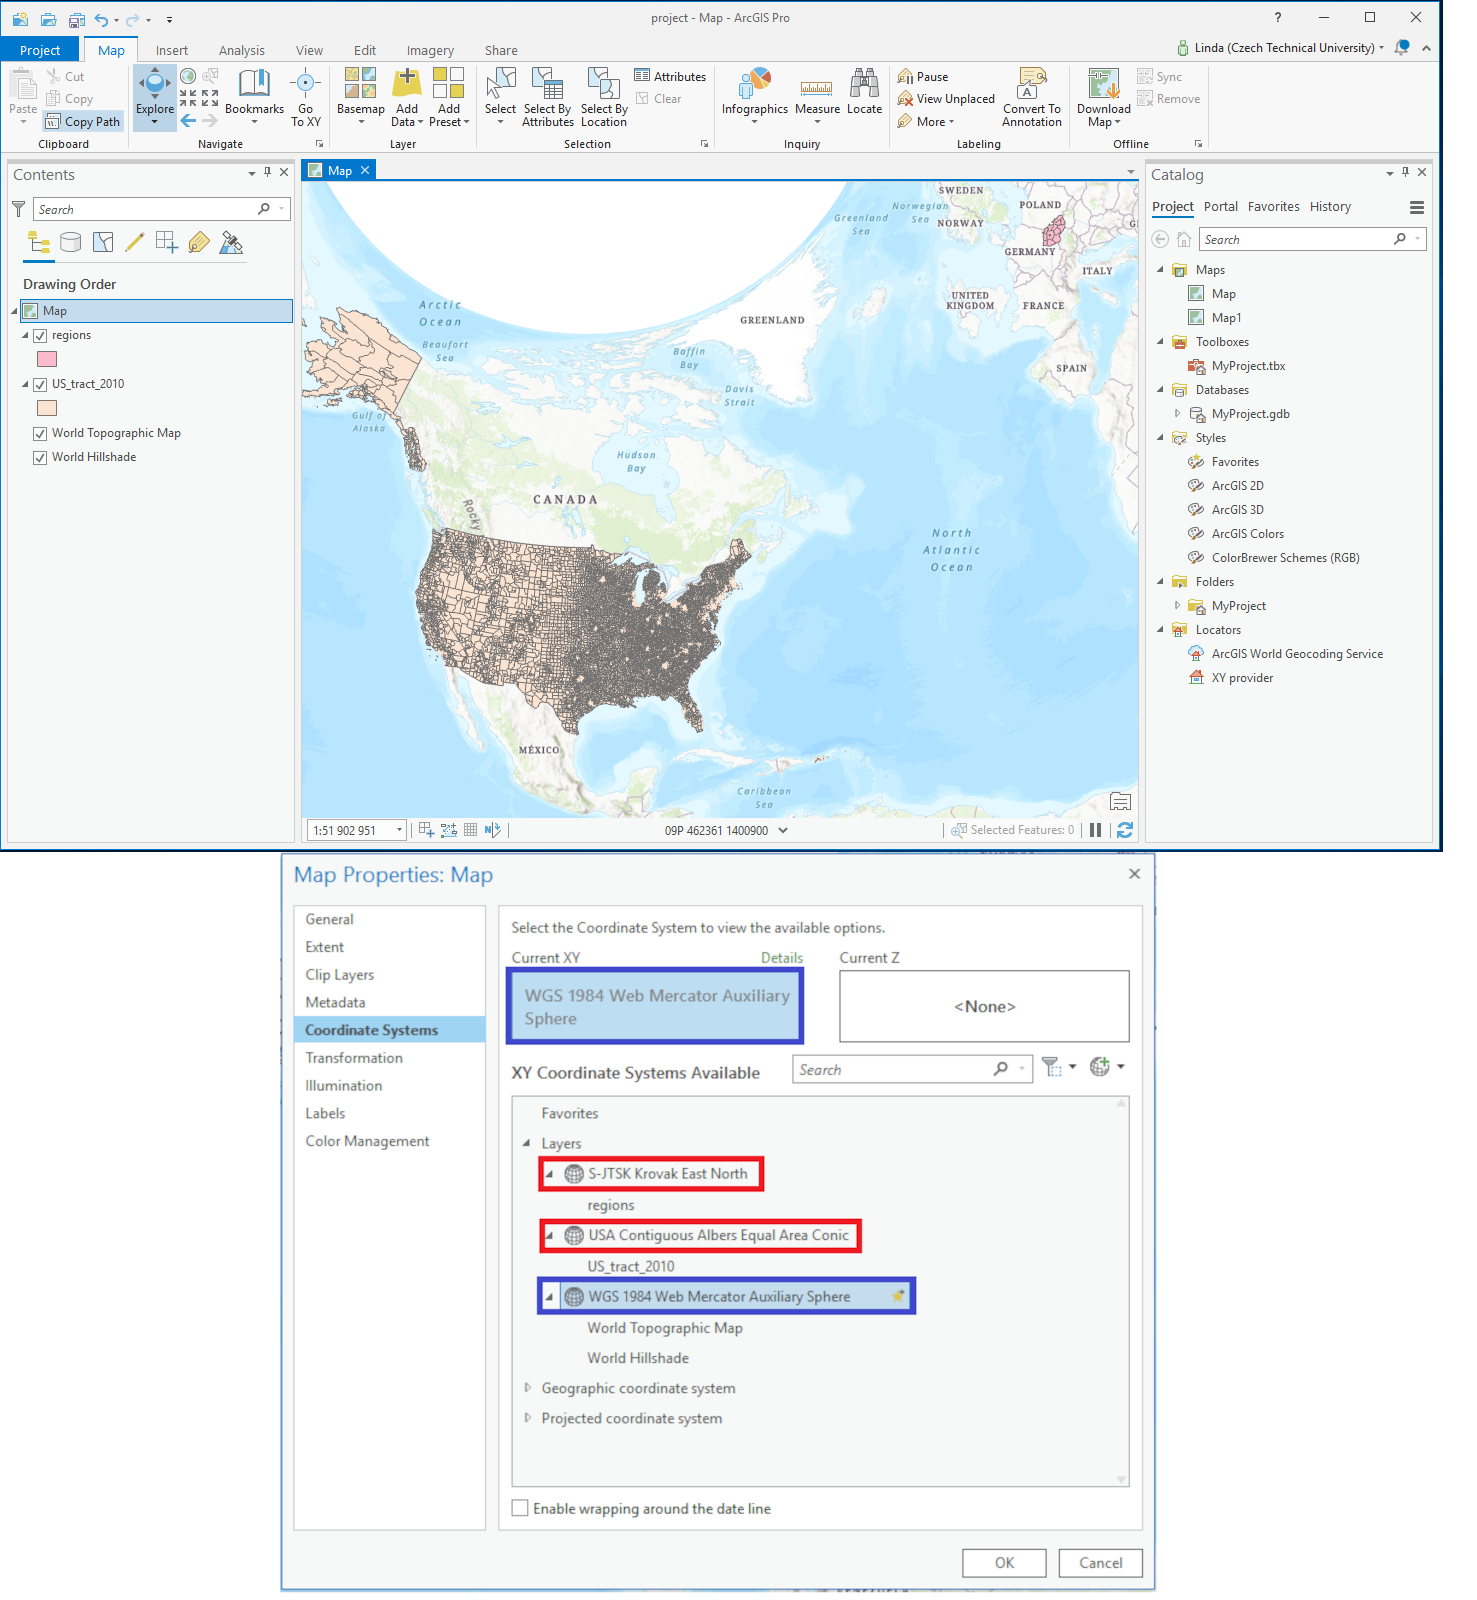
\includegraphics[width=15cm]{../pictures/arcgis_pro_onthefly2.png} 
\caption[Display of layers with different coordinate system in ArcGIS Pro 2.4 (source own)]{Display of layers with different coordinate system in ArcGIS Pro 2.4 (source own)}
\label{fig:arcgis_pro_onthefly2}
\end{center}
\end{figure}

\noindent ArcGIS Pro pracuje s projekty jako hlavními prvky organizace dat. Každý projekt obsahuje složku, která obsahuje data, s nimiž chceme pracovat. Je zde tedy tlak na to, aby data měla své jasné místo a nebyla rozházena všude po disku. Můžeme říci, že společnost ESRI jde v tomto aspektu podobným směrem jako GRASS GIS. V případě tohoto softwaru není mínusem, že nenabízí žádné zvláštní prvky nebo vysvětlivky, které by mohly pomoci newcomers. Startovací obrazovka i software jako takový je na první pohled přehledný a user friendly.

\bigskip

\noindent \textbf {GeoMedia Advantage 2020}

\noindent This commercial GIS software is developed by  Intergraph (now Hexagon Geospatial) has  a rich 40-year history. It is especially strong at cartography and raster analysis.  It also offers a unique 3D experience for viewing and analyzing data.

Po složitém nastavením licencí (není možné vyzkoušet jednoduše trial verzi, je nutné si zažádat o časově omezený licenční klíč), nás uvítá malý startovací dialog na obrázku \ref{fig:geomedia_startup}, kde si můžeme vytvořit vlastní GeoWorkspace file nebo otevřít stávající. 

\vspace{0.3cm}
\begin{figure}[hbt!] 
\begin{center}
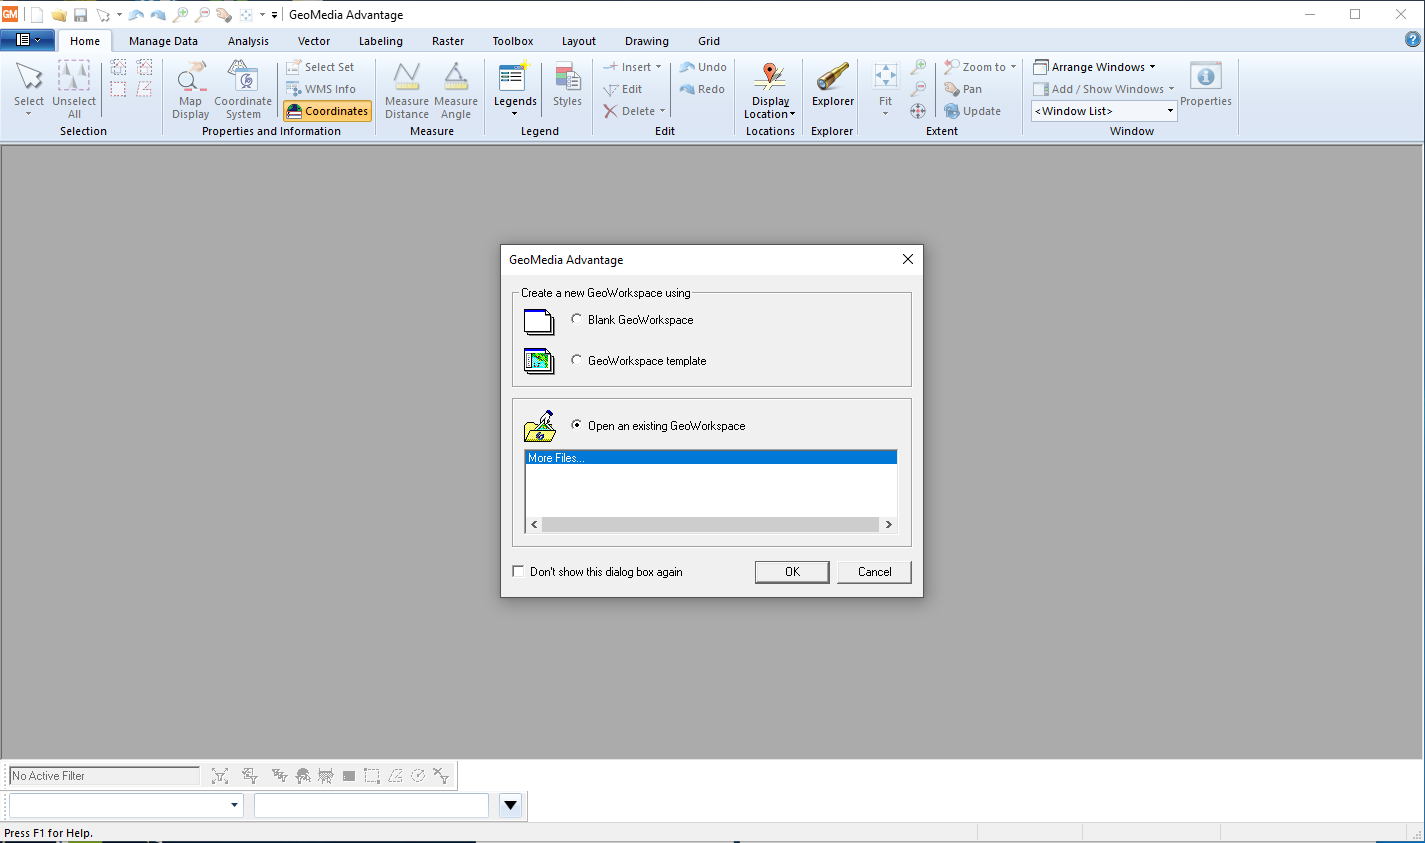
\includegraphics[width=15cm]{../pictures/geomedia_startup.png} 
\caption[GeoMedia Advantage 2020: startup dialog (source own)]{GeoMedia Advantage 2020: startup dialog (source own)}
\label{fig:geomedia_startup}
\end{center}
\end{figure}

\noindent Software naštěstí poskytuje dva příklady GeoWorkspace projektů, což dá alespoň menší představu o tom, jak to celé funguje. Nicméně, pokud chceme přidat vlastní data, je to velmi uživatelsky nepřívětivé a autorce se to podařilo až po půl hodině intenzivního snažení. 

Jakákoli externí data, které chceme do softwaru přidat, mají charakter Warehouses. Aby bylo možné například zobrazit shapefile (ale i jiné formáty), je nutné si neprve definovat Warehouse Configuration File. Ten se skládá z definice datového serveru (v případě shapefilu ArcView), pracovní složky s daty a z definice souřadnicového systému, viz obrázek \ref{fig:define_config_geomedia}. GeoMedia rovněž jako GRASS požaduje, aby uživatel od začátku definoval, v jakém systému pracuje a poskytuje pro tento účel velmi podrobné nastavení.

\vspace{0.3cm}
\begin{figure}[hbt!] 
\begin{center}
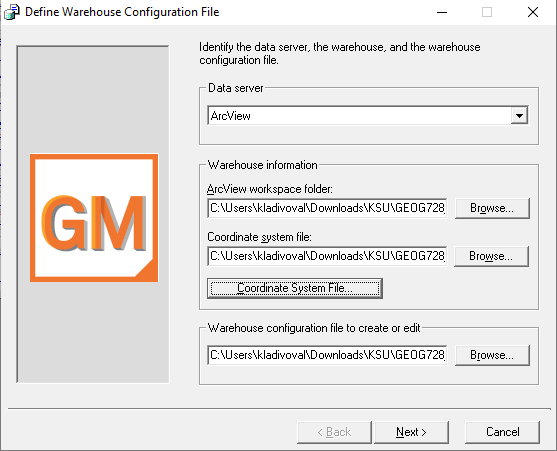
\includegraphics[width=12cm]{../pictures/define_config_geomedia.png} 
\caption[GeoMedia Advantage 2020: Define Warehouse Configuration File dialog (source own)]{GeoMedia Advantage 2020: Define Warehouse Configuration File dialog (source own)}
\label{fig:define_config_geomedia}
\end{center}
\end{figure}

\noindent V dalším kroku je nutné si tento konfigurační soubor připojit. Once it is connected a user can manipulate with data in a map window as with legend entries. Každý GeoWorkspace file může mít připojeno více Warehousů s různými souřadnicovými systémy. V mapovém okně pak dochází k On the fly transformaci podle souřadnicového systému mapového okna, který se nastavuje pod pojmem Lokace. 

Software neposkytuje žádnou nápovědu, uživatel je tak naprosto bezradný a donucený hledat na internetu. Z hlediska učení je tento software rozhodně z vybraných třech komerčních softwarů nejnáročnější na prvotní pochopení. Můžeme nicméně vnímat jistou podobnost s GRASSem, a to zejména v nastavení souřadnicového systému, které je rovněž velmi podstatné zhlediska GeoMedia softwaru.  Mapové okno nicméně podporuje On the fly transformaci, což je výrazná odlišnost od GRASS GIS.

\newpage
\vspace*{-1cm}
\bigskip

\noindent \textbf {MapInfo Professional 2019}

\noindent This commercial GIS software is developed by the American company Pitney Bowes, in the Czech Republic the exclusive provider is CS Map. As the name suggests, MapInfo is very strong in geodata visualization. it offers functionalities for doing modern cartography - several prepared map layouts, advanced labelling, accessing symbology etc. However, some analytical functions e. g. focused on LiDAR and remote sensing are missing.

When we run the software, we are redirected to the Startup screen, which atypically occupies the size of the entire computer screen. The startup provides links to new version news or links to videos on YouTube that can help first-time users. In the upper right part of the startup screen it is possible to run help, which has the character of a separate desktop application. In the left part there is a simple bar allowing to choose a workspace we want to work in. We can open an empty workspace, sample workspace with a map of Washington DC or choose another previously saved workspace in the directory path. If we run the software again, the Open Last Saved Session option will be added to the startup screen.

\vspace{0.3cm}
\begin{figure}[hbt!] 
\begin{center}

\includegraphics[width=14.5cm]{../pictures/map_info_startup_screen.PNG} 
\caption[MapInfo Professional 2019 startup dialog (source own)]{MapInfo Professional 2019 startup dialog (source own)}
\label{fig:map_info_startup_screen}
\end{center}
\end{figure}

\noindent As in ArcGIS Pro, the main component is the Map, which has one coordinate system defined. Data import is somewhat non-intuitive and must be demonstrated through the Open Table icon. When importing, a new file of company's own geodata format * .tab is created. We can define new projection or keep the original one. Coordinate system of the Map can be changed through Map Options as shown on Figure \ref{fig:map_info_startup_projection}. 

\vspace{0.3cm}
\begin{figure}[hbt!] 
\begin{center}
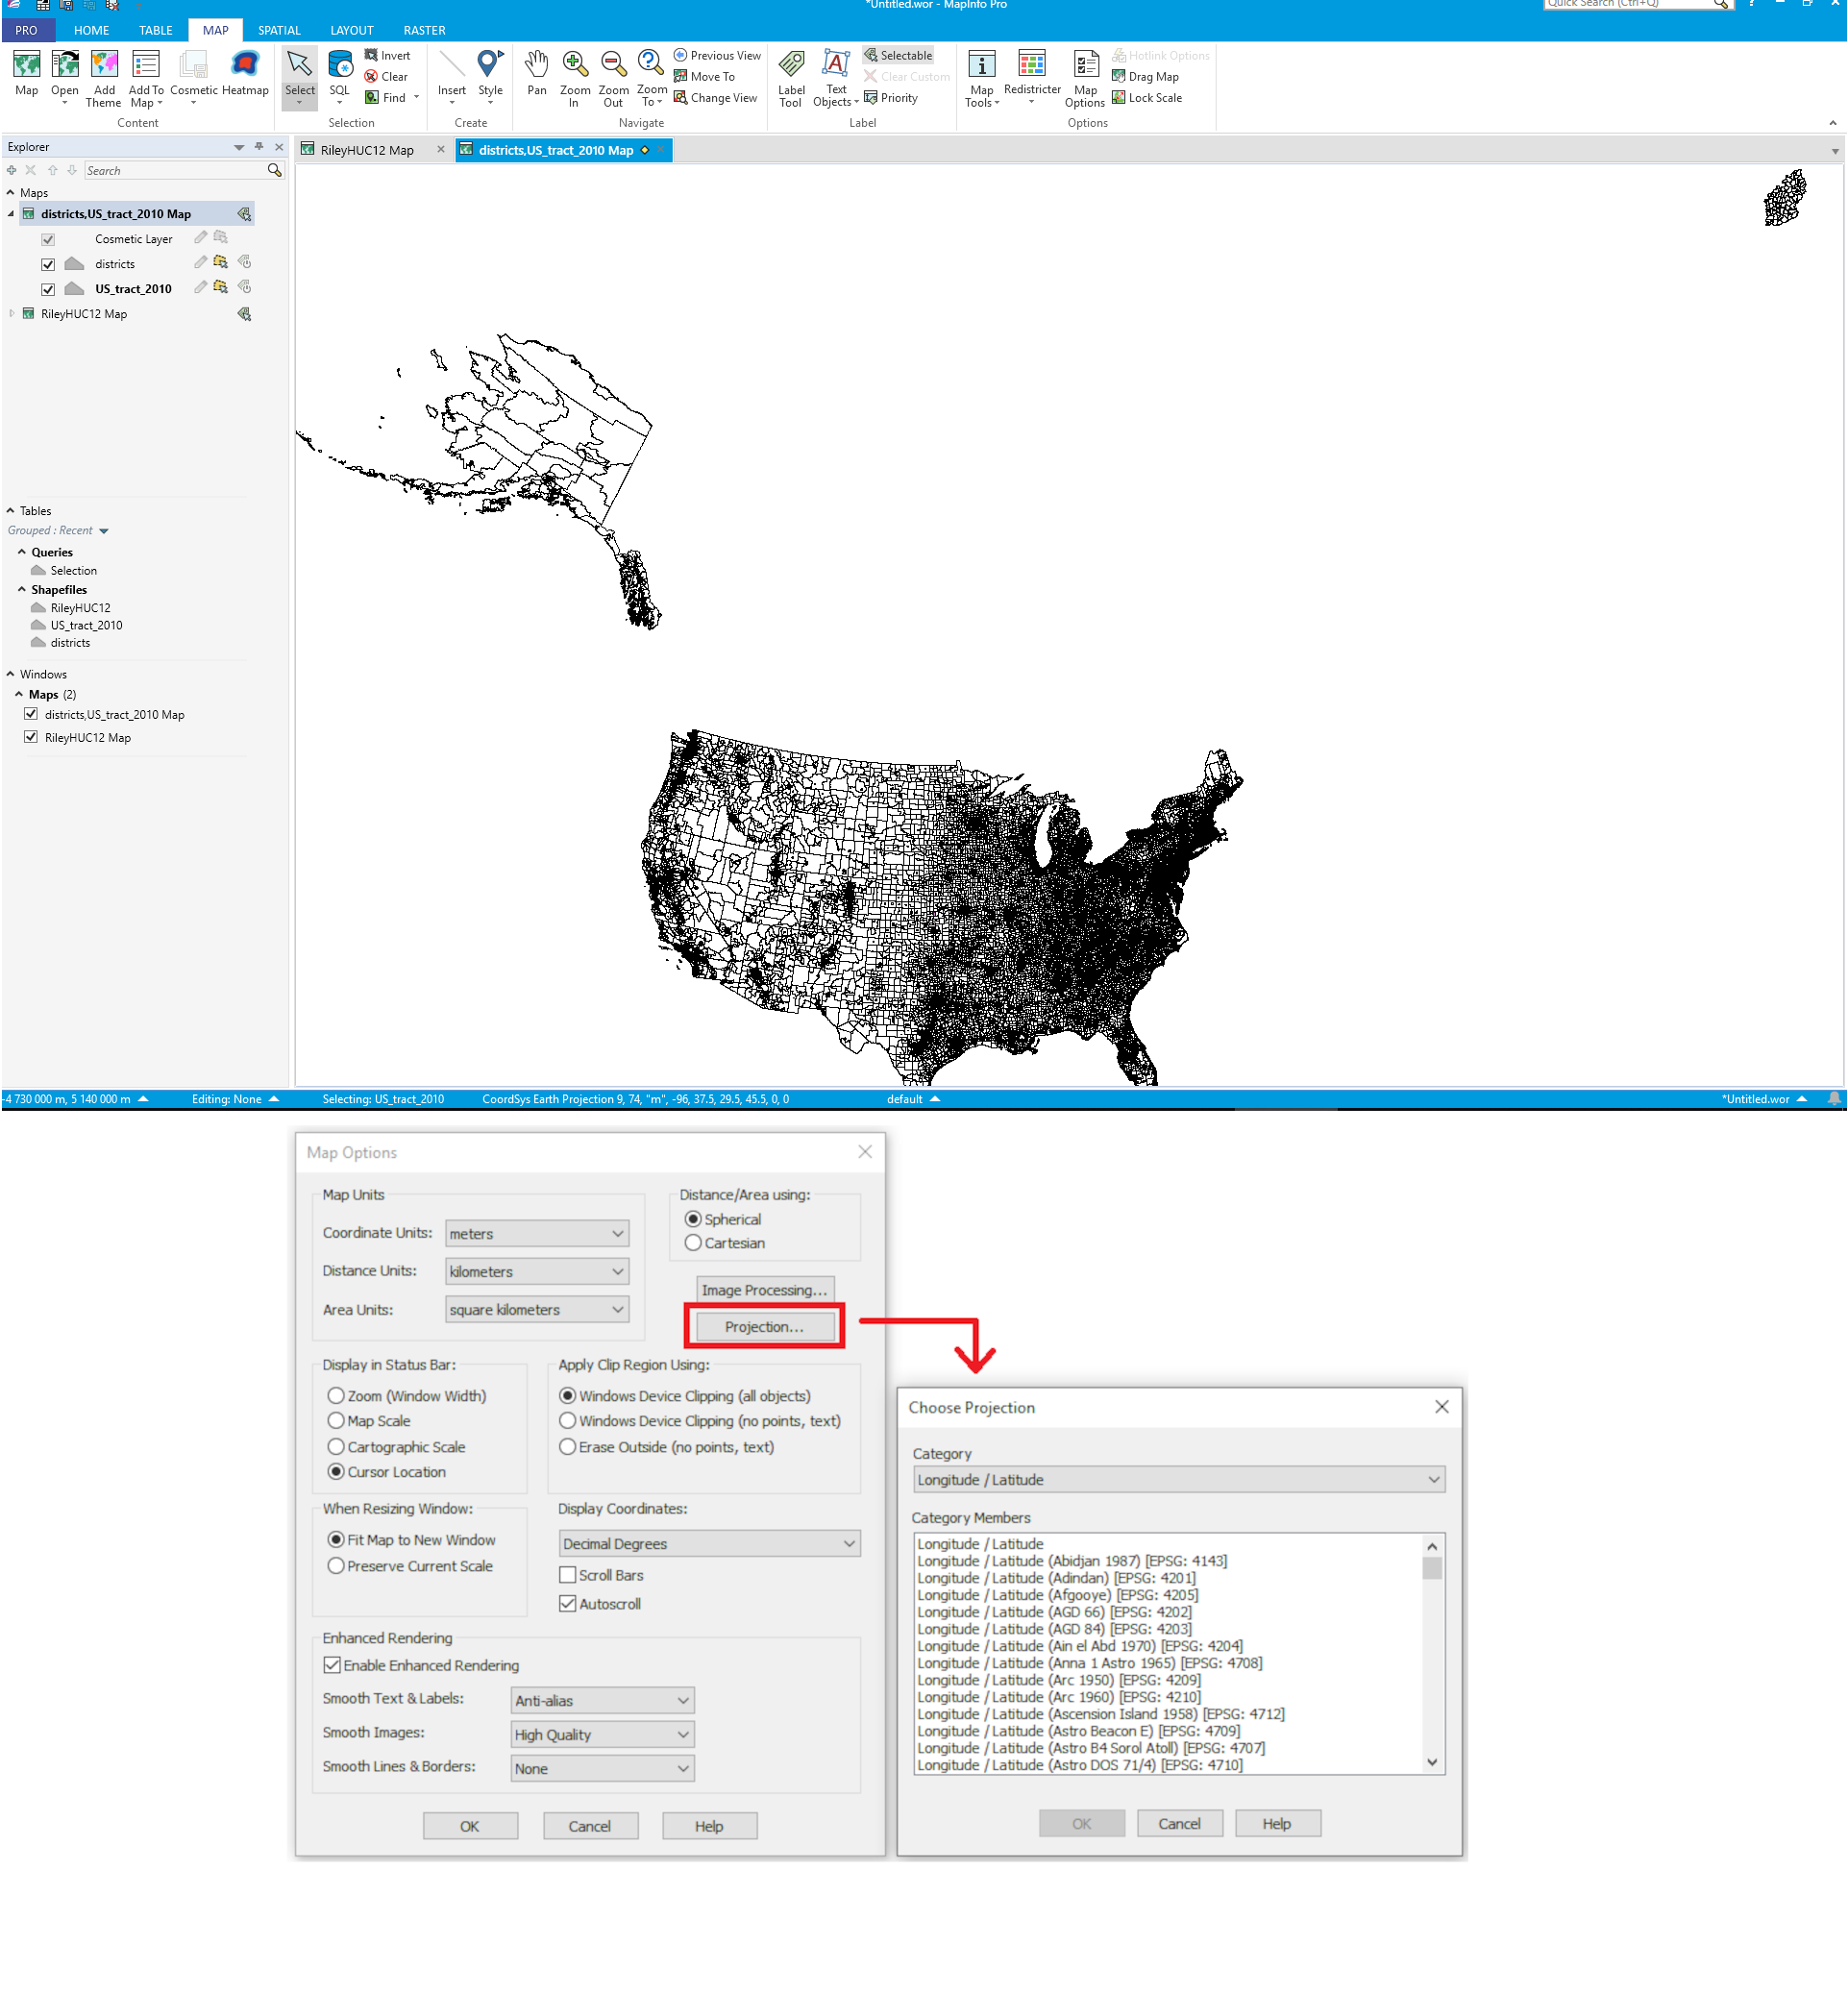
\includegraphics[width=15cm]{../pictures/map_info.PNG} 
\caption[Map-level coordinate system settings in MapInfo Professional 2019 (source own)]{Map-level coordinate system settings in MapInfo Professional 2019 (source own)}
\label{fig:map_info_startup_projection}
\end{center}
\end{figure}

\noindent However, at first glance it is not clear in which coordinate system the layers are, more precisely whether we made On the fly transformation or data transformation. After a longer examination, it is clear that we transformed MapInfo *.tab file. The coordinate system is set to the map level (not layer level) and takes over the system of the first map layer added. 

\newpage
\vspace*{-1cm}
\subsubsection{Analysis of selected open-source software}

\noindent On further rows four open-source software (QGIS 3, gvSIG, ILWIS, SAGA GIS) are tested and analyzed in detail from the point of view of the startup mechanism with an emphasis on finding out what elements they use directly in the software to improve the first-time user experience. V další kapitole jsou poté výsledky těchto analýz shrnuty do tabulek. 

\bigskip

\noindent \textbf {QGIS 3.14}

\noindent This software is created similarly to GRASS GIS under the auspices of OSGeo. The big change from QGIS 2 is that it includes native support for 3D visualizations. The advantage is also the possibility of using and creating tailor-made plugins. QGIS also allows the use of analytical functions from GRASS, SAGA GIS software and the GDAL library. 

At the first start, Welcome to QGIS window appears, in which we can link to the QGIS website and check the news in the given version. The window runs in the default language of the operating system.

\vspace{0.3cm}
\begin{figure}[hbt!] 
\begin{center}
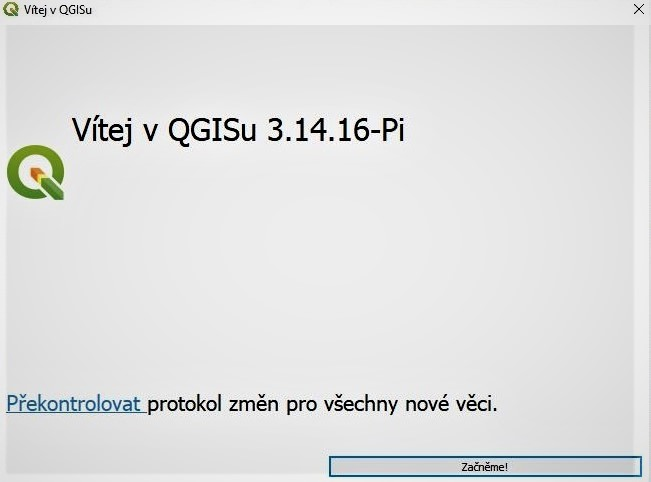
\includegraphics[width=8.5cm]{../pictures/qgis_startup_window.JPG} 
\caption[Welcome to QGIS 3.14 window (source own)]{Welcome to QGIS 3.14 window (source own)}
\label{fig:qgis_startup_window}
\end{center}
\end{figure}

\noindent After this introduction, we are redirected to the main software window (Fig. \ref{fig:qgis_first_window})  informing about community events and significant improvements that have taken place. Here we can choose an empty project template or we may open sample datasets (North Carolina, South Dakota, Alaska) provided along with instalation.

In QGIS 3, we distinguish between the layer's and project's CRS. It is worth mentioning that QGIS supports about 2700 known coordinate systems, whose definitions are stored in the SQLite database installed together with QGIS. The empty project has always global default projection EPSG: 4326 - WGS 84.

\vspace{0.3cm}
\begin{figure}[hbt!] 
\begin{center}
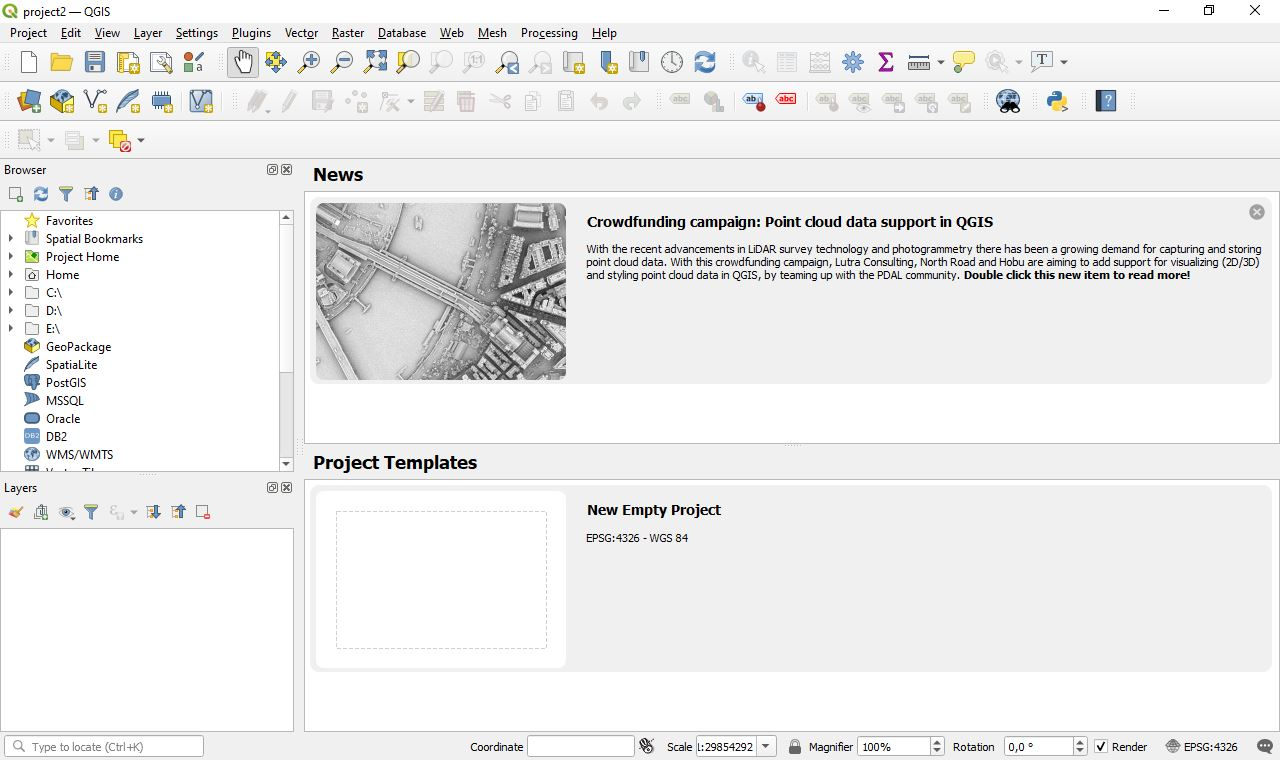
\includegraphics[width=15cm]{../pictures/qgis_first_window.JPG} 
\caption[The main software window after first opening QGIS 3.14 (source own)]{The main software window after first opening QGIS 3.14 (source own)}
\label{fig:qgis_first_window}
\end{center}
\end{figure}

\noindent In QGIS, On-the-fly transformation is enabled by default, meaning that whenever you use layers with different coordinate systems QGIS transparently reprojects them to the project CRS. When importing the first layer (in this case US tracts in ESRI: 102003 system), the dialog box shown in Fig. \ref{fig:qgis_transformation} specifies what type of transformation to perform when changing the project CRS. These Datum transformations are then listed in Project Properties - CRS settings (Fig. \ref{fig:qgis_trans}). It is important to note that the first layer added defines the coordinate system of the project. In our case, it was changed to the US Contiguous Albers Equal Area Conic system. In the dialog \ref{fig:qgis_trans} we can set the Predefined coordinate system, which is related to the project, not to the layer.

Whenever a more accurate transformation is available, but is not currently usable, QGIS 3 shows an informative warning message (see Fig. \ref{fig:qgis_warning_window}) advising to use more accurate transformation. Those messages appear quite often in a variety of situations, which can help significantly new as well as experienced users.

\begin{figure}[hbt!] 
\begin{center}

\includegraphics[width=15cm]{../pictures/qgis_warning_window.JPG} 
\caption[Informative warning message  in QGIS 3.14 (source own)]{Informative warning message  in QGIS 3.14 (source own)}
\label{fig:qgis_warning_window}
\end{center}
\end{figure}

\begin{figure}[hbt!] 
\begin{center}
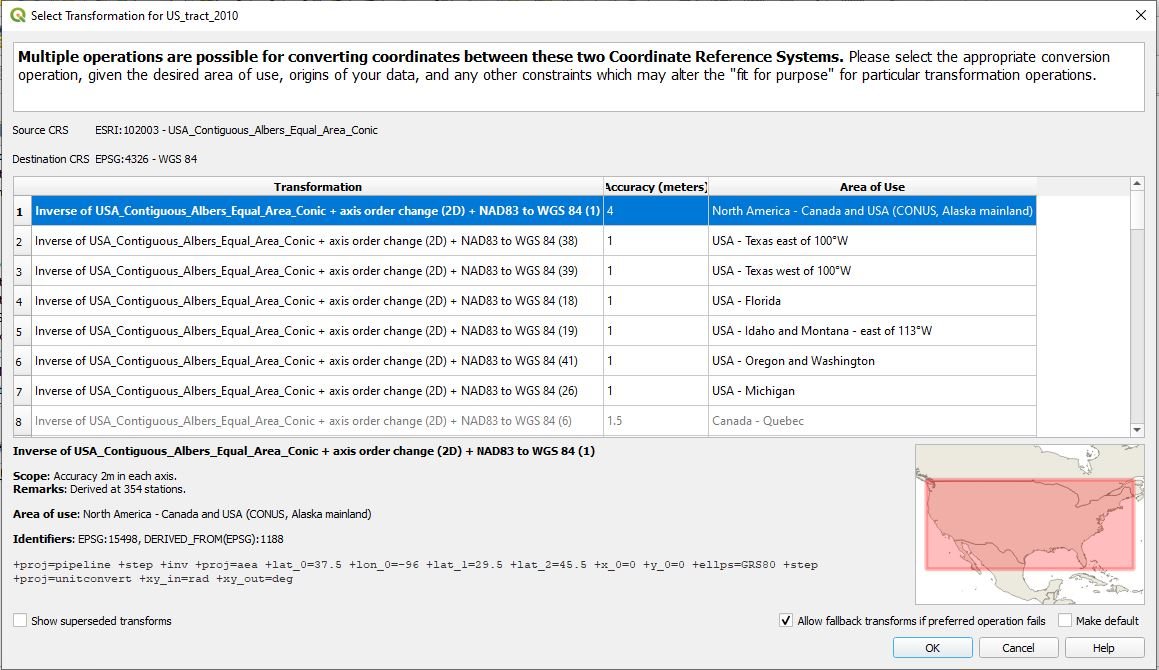
\includegraphics[width=14cm]{../pictures/qgis_transformation.JPG} 
\caption[Correct display of layers with different coordinate system in gvSIG 2.5.0 (source own)]{Correct display of layers with different coordinate system in gvSIG 2.5.0 (source own)}
\label{fig:qgis_transformation}
\end{center}
\end{figure}

\begin{figure}[hbt!] 
\begin{center}
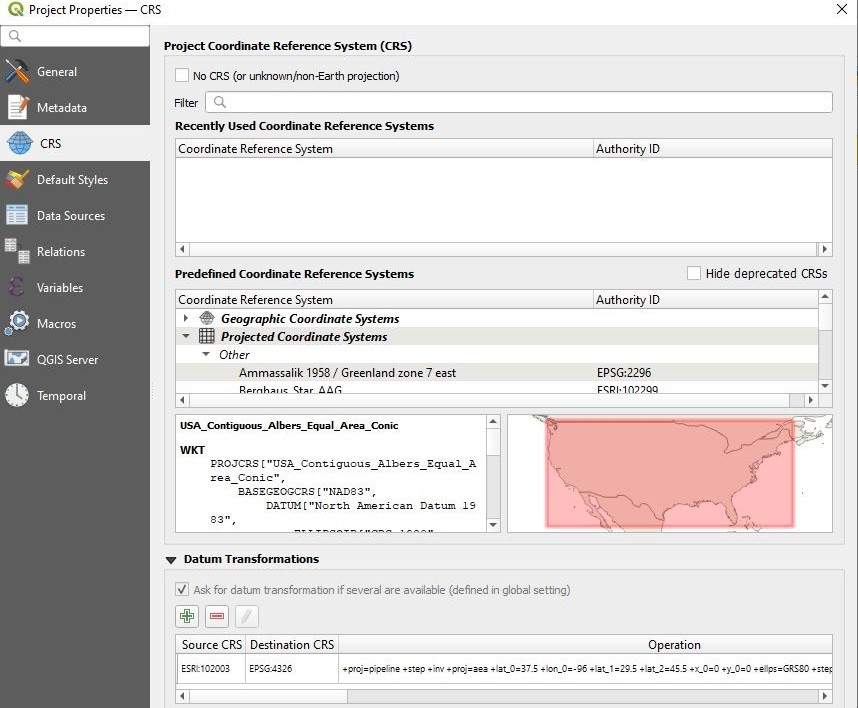
\includegraphics[width=14cm]{../pictures/qgis_trans.JPG} 
\caption[Predefined CRS and Datum Transformations in QGIS 3.14 (source own)]{Predefined CRS and Datum Transformations in QGIS 3.14 (source own)}
\label{fig:qgis_trans}
\end{center}
\end{figure}


\newpage
\vspace*{-1cm} 
\bigskip

\noindent \textbf {gvSIG 2.5.0}

\noindent Here we will describe the startup mechanism of another open-source software created under the OSGeo organization. gvSIG can work with common vector and raster data, integrates files and databases as well as remote data through OGC standards. It is developed in Java and, like QGIS, includes a plugin system which allows to easily extend the software capabilities and develop tailor-made solutions.

Software is designed very simply. It does not have a startup window, nor does it support any first-time mode. When started, an empty map window will open. The work is saved in a project with the extension * .qvsproj, which can then be started through the associated icon. If we do not start the software using the project's association icon, it is reopened by default with a blank map. Adding layers is also intuitive. It is possible to add multiple layers in different coordinate systems, the software recognizes the EPSG codes. The data still retains its original coordinate system, however, map layers are rendered in the WGS 84 (EPSG:4326) using On the fly transformation, see Fig. \ref{fig:gvSIG_coords}.

\vspace{0.3cm}
\begin{figure}[hbt!] 
\begin{center}
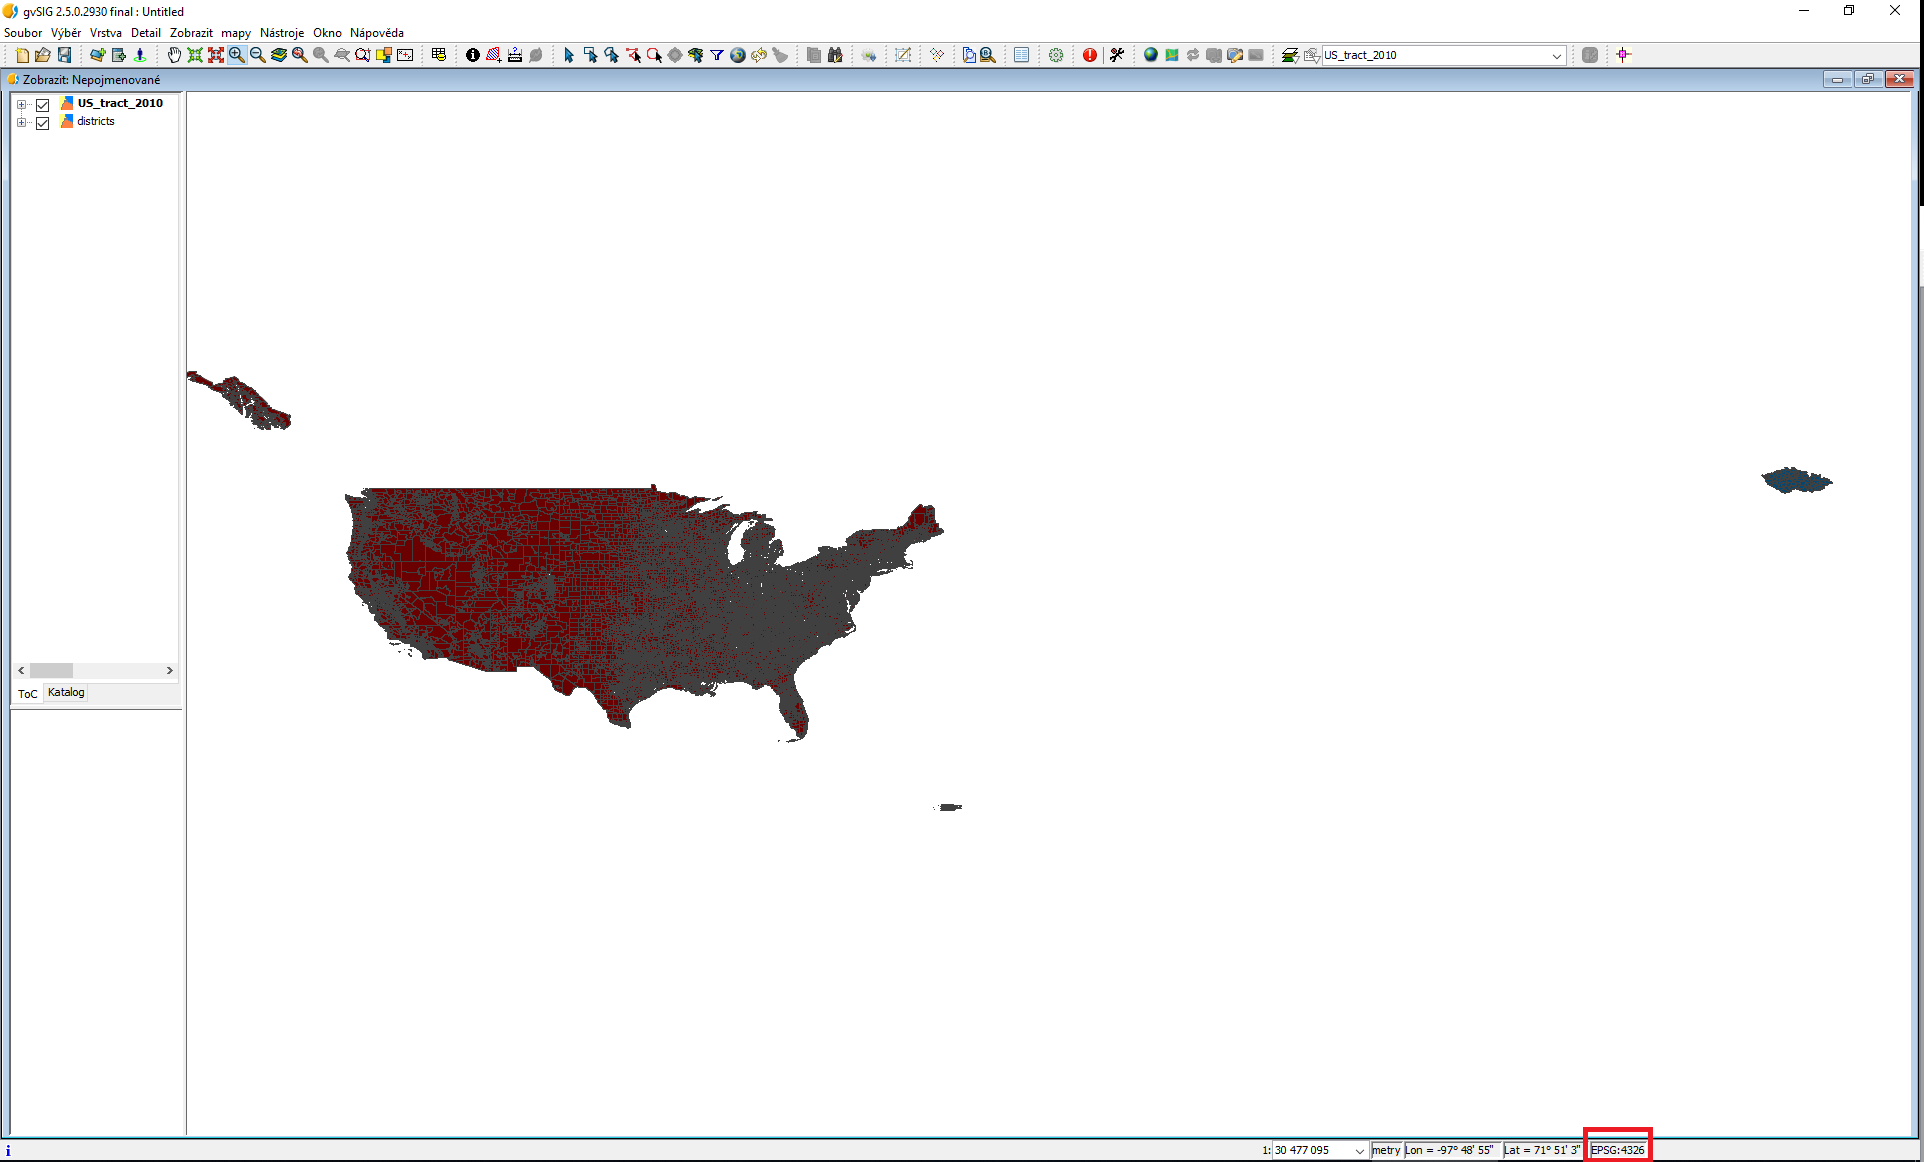
\includegraphics[width=15cm]{../pictures/gvSIG_coords.PNG} 
\caption[Correct display of layers with different coordinate system in gvSIG 2.5.0 (source own)]{Correct display of layers with different coordinate system in gvSIG 2.5.0 (source own)}
\label{fig:gvSIG_coords}
\end{center}
\end{figure}

\bigskip

\noindent \textbf {ILWIS 3.3 (Integrated Land and Water Information System)}

\noindent The strong point of this system developed at University of Twente in the Netherlands has always been remote sensing and hydrological flow operations.

The software starts without a startup window and does not have features enhancing first-time user experience. On the left there is a section with several tabs: Operation-Tree, Navigator and Finder. ILWIS seems to be very similar to GRASS GIS. Operation-Tree and Finder are defacto the Modules tab in GRASS divided into two sub-tabs.  The data is similarly to GRASS stored in the home directory here called Data, which is taken as the default when importing or creating data. The content of this folder is in special formats that ILWIS understands, see Figure \ref{fig:ilwis_uvodni_okno}. 

The navigator has a tree structure like the GRASS Data Catalog and represents the entire directory structure, not just a home Data directory. ILWIS does not have its own native file to save the projects or workspaces.

\vspace{0.3cm}
\begin{figure}[hbt!] 
\begin{center}
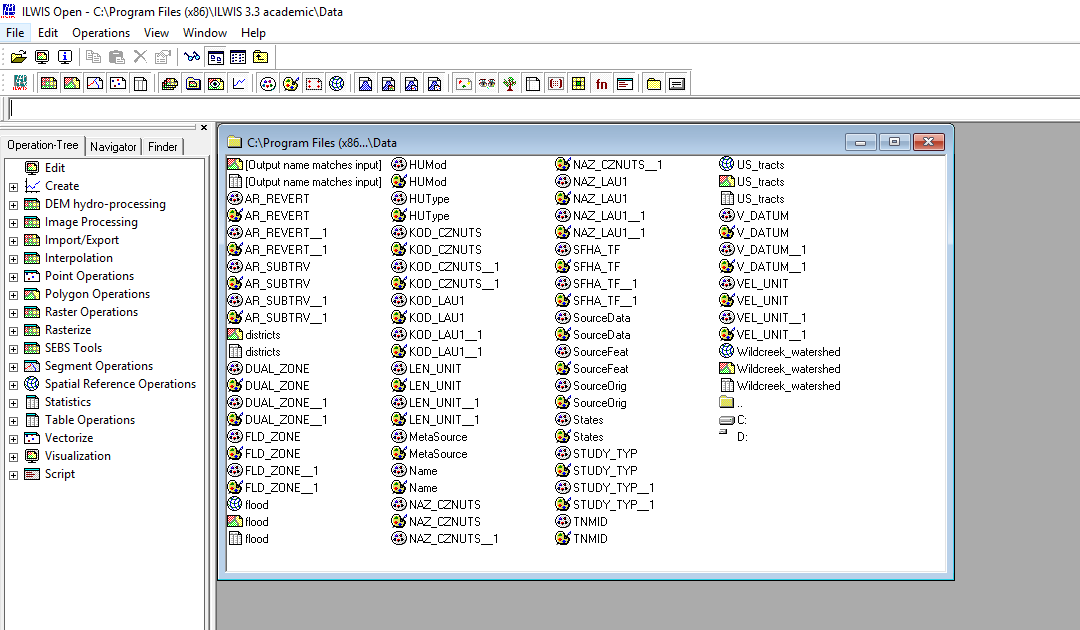
\includegraphics[width=15cm]{../pictures/ilwis_uvodni_okno.png} 
\caption[The main software window after reopening ILWIS 3.3 (source own)]{The main software window after reopening ILWIS 3.3 (source own)}
\label{fig:ilwis_uvodni_okno}
\end{center}
\end{figure}

\noindent The display of layers with different coordinate system is tested as well. Importing data in the form of a shapefile is somewhat unintuitive here. If we want to perform an import we might go to the Operation-Tree $->$ Import/Export $->$ Import Map, however we encounter the problem that the software does not know the shapefile format. Therefore, the second option can be found in the top bar File $->$ Import. Here we select the ESRI shapefile and it is necessary to expand the default output so that the imported file is saved as an ILWIS object with the * .ioc extension. If we do not do this, only the tables will be imported, no maps.

It is interesting how the software approaches coordinate systems. When importing the layer called districts, the S-JTSK Krovak East North system is converted to the Unknown. In case of US tracts, the US Contiguous Albers Equal Area Conic system is converted to the LatLon system. Therefore, the software does not carry information about a specific coordinate system, it only cares about boundaries of the map. When displaying multiple layers with different coordinate systems in one map window, no On the fly transformation is performed. The system gets confused and the added layer is not displayed even after clicking on the ''Zoom to Layer'' function. There is no need to save the software, after opening it reflects the current state of the Data folder.

\vspace{0.3cm}
\begin{figure}[hbt!] 
\begin{center}
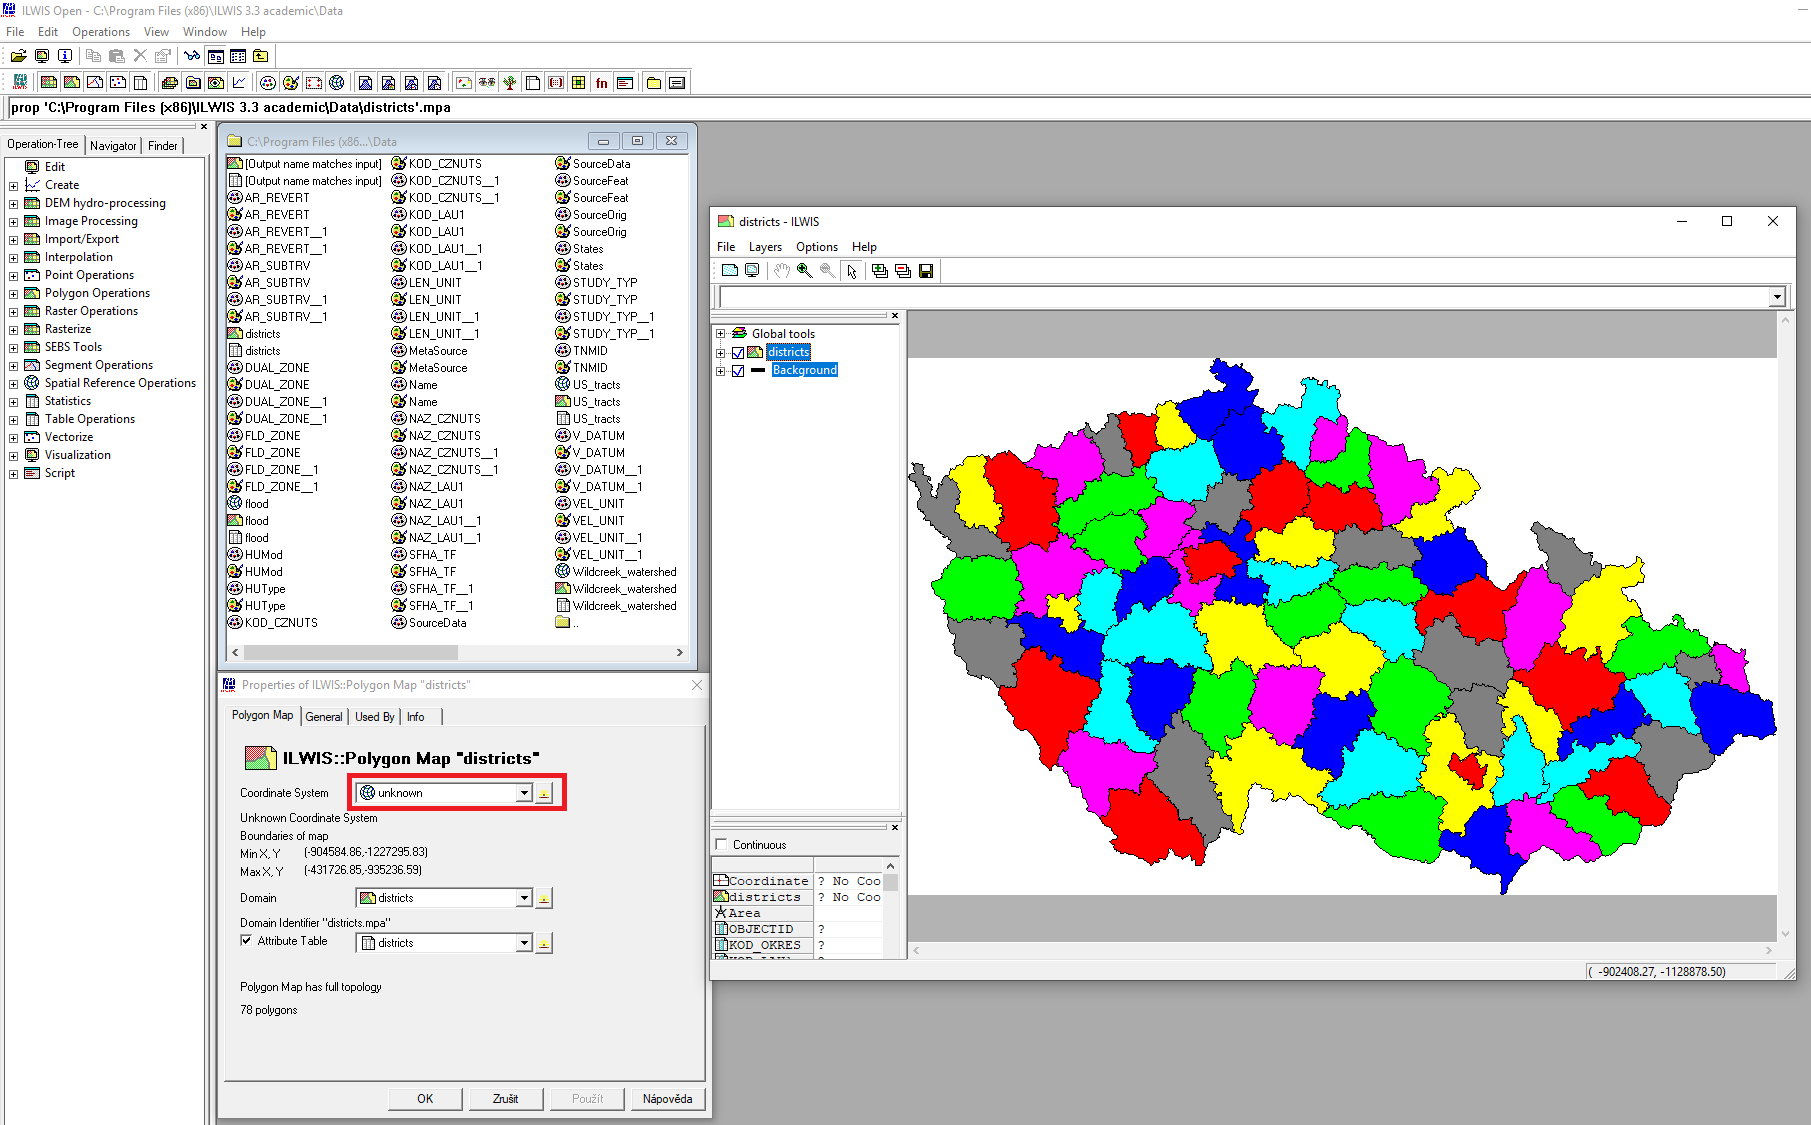
\includegraphics[width=15cm]{../pictures/ilwis_pridani_mapy.png} 
\caption[Unknown coordinate system properties of district layer in ILWIS 3.3 (source own)]{Unknown coordinate system properties of district layer in ILWIS 3.3 (source own)}
\label{fig:ilwis_pridani_mapy}
\end{center}
\end{figure}

\bigskip

\noindent \textbf {SAGA GIS 2.3 (System for Automated Geoscientific Analyses)}

\noindent SAGA GIS is a Free Open Source Software (FOSS) offering a comprehensive, growing set of higher-level geoscientific methods. It is one of the most favorite software for remote sensing needs because of its rich library grid, imagery and terrain processing modules.

This software is blank the first time it is run. On the left there is a window with the Tools, Data and Maps tabs, which are similar to the Modules, Data, Layers tabs in GRASS GIS 7.8. The Data and Maps tabs are further divided into the Tree and Thumbnails subtabs. The tree is divided according to the shapes of geometric objects (point, line, polygon ...). 

The idea is different from GRASS GIS. The directory structure of added layers is always displayed for the current layer in the lower left window of Data Sources in the File System tab. So we do not have a specific folder in which we work from the beginning. We can add layers to the tree structure and the whole project will be created only when we save the settings to a SAGA GIS project file.

In the Maps tab, multiple layers can be displayed on top of each other or a new map map window can be created for each layer, which is a default option. However, there is no On the fly transformation. It means that layers with different coordinate systems may be displayed at the level of one map.  As we can see in Figure \ref{fig:saga_gis_cele}, the Czech Republic appears next to the American continent, as the system assumes adding layers with the same coordinate system to the map.

\begin{figure}[hbt!] 
\begin{center}
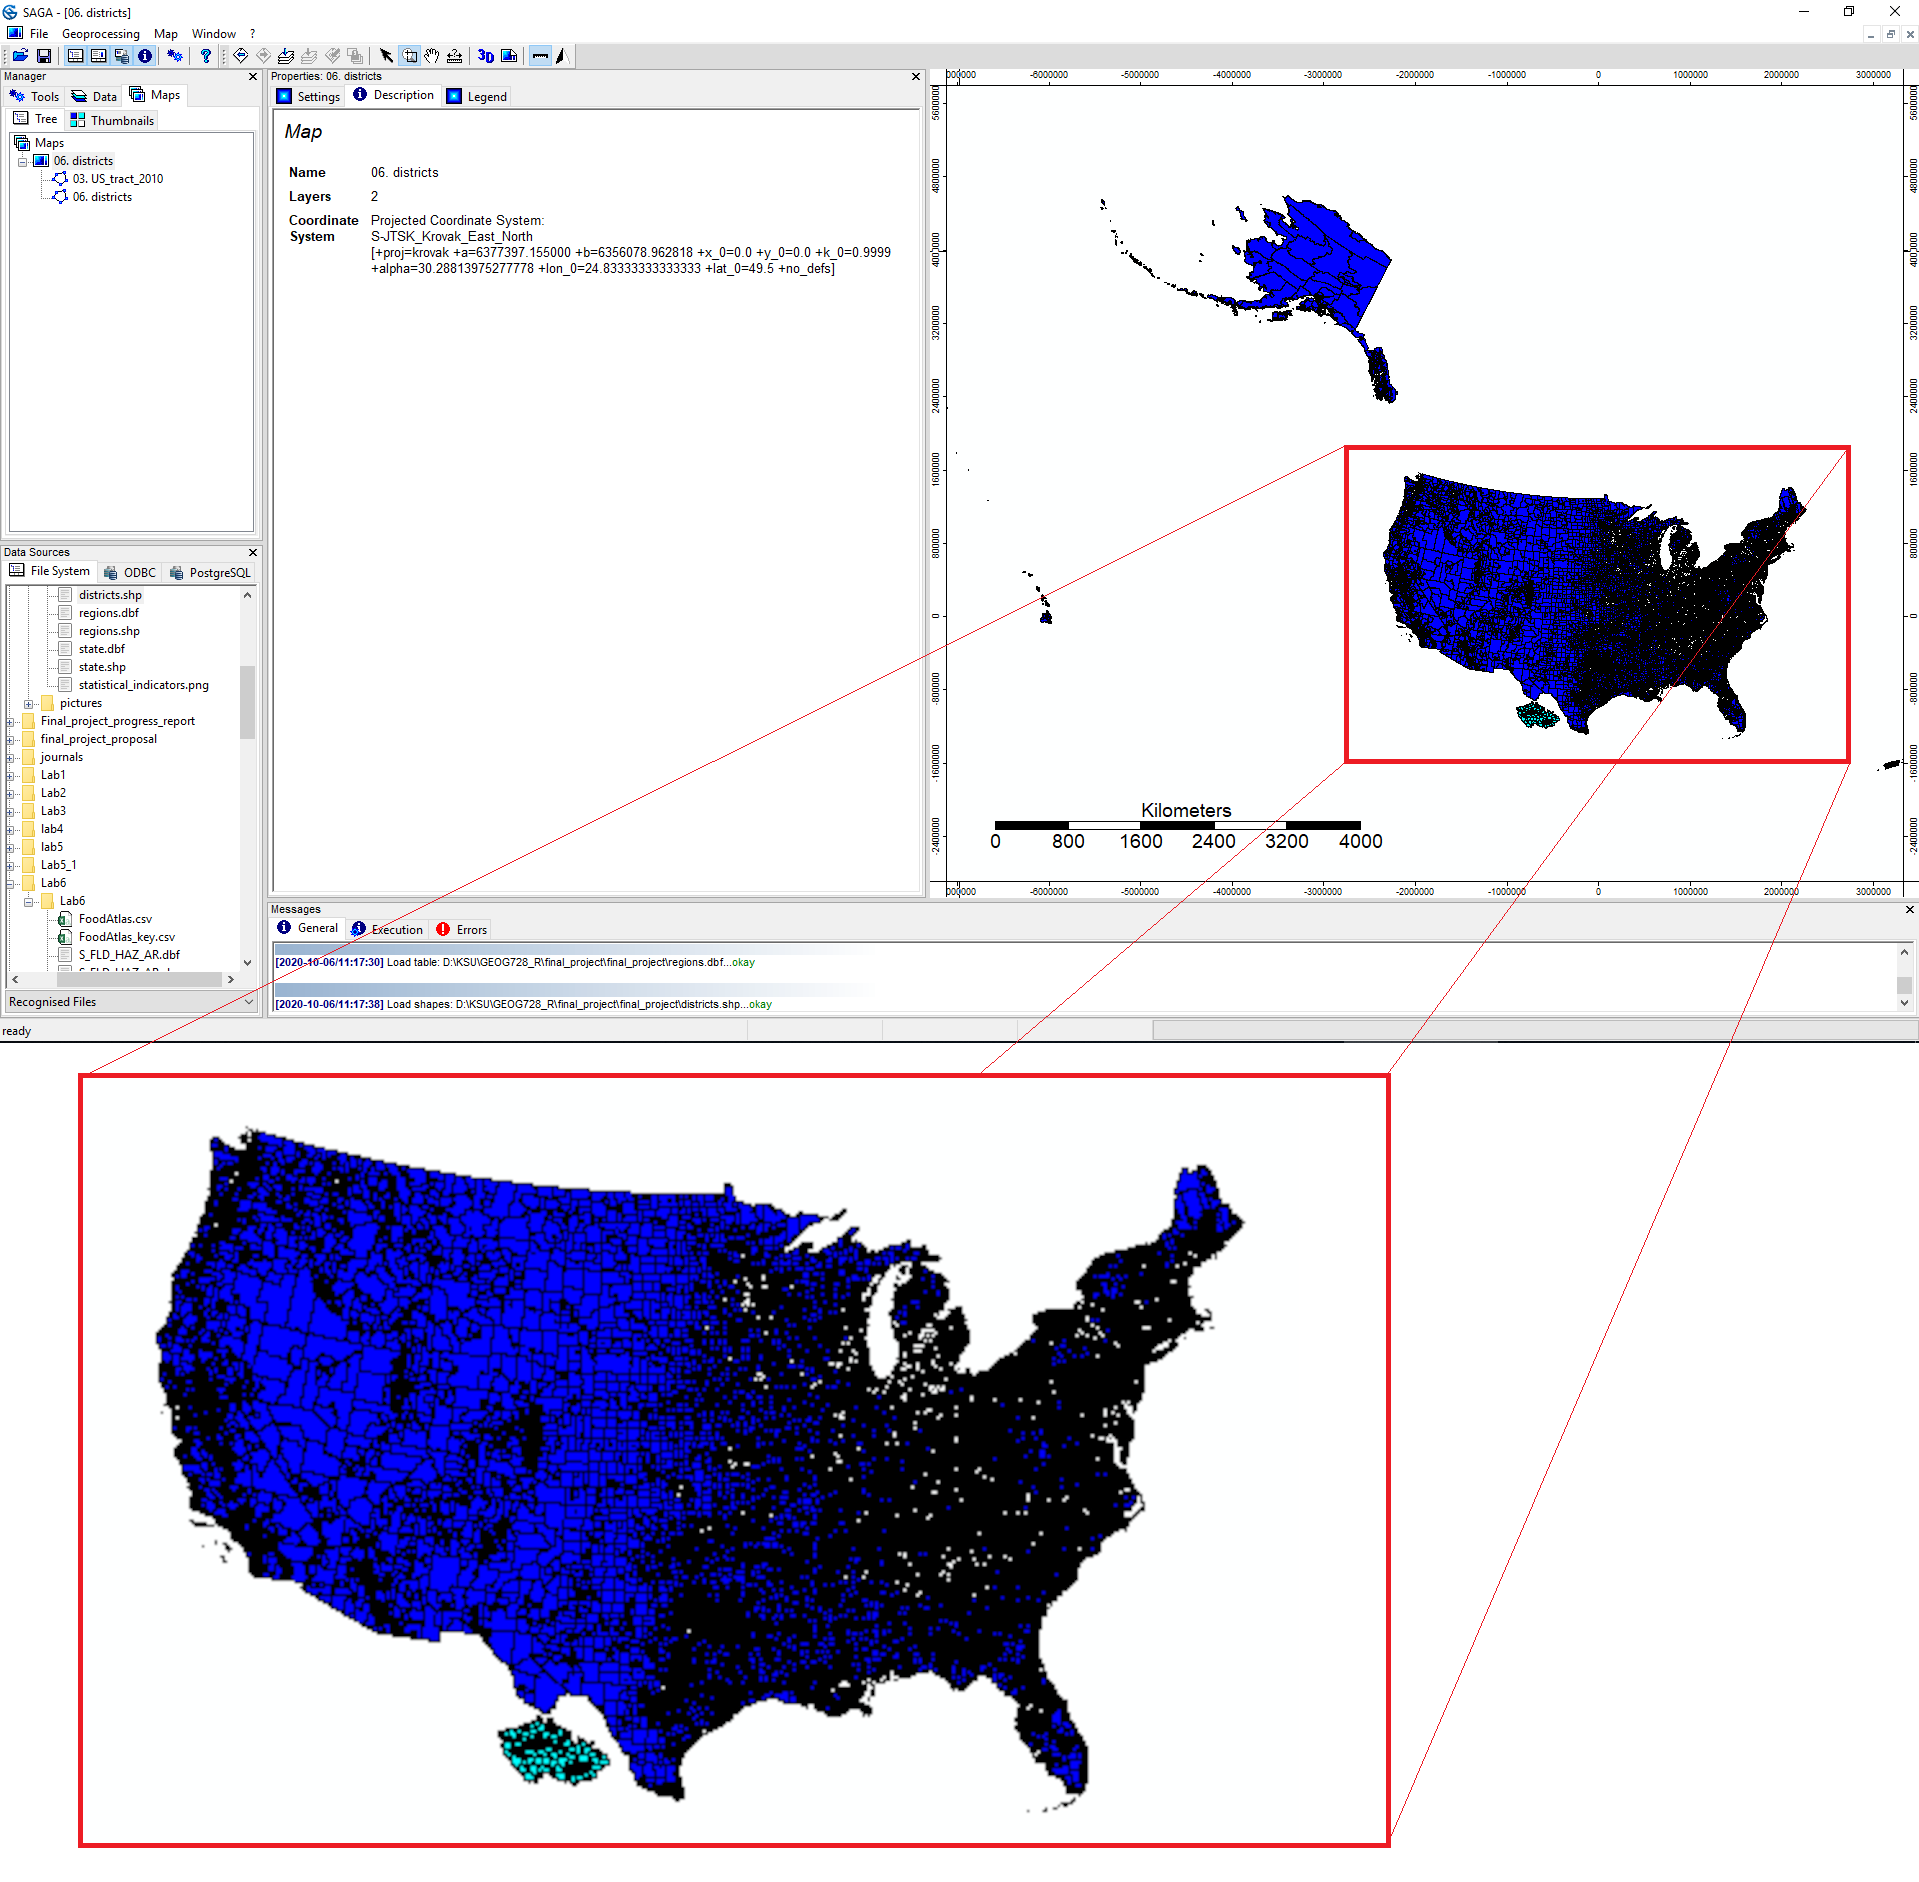
\includegraphics[width=15cm]{../pictures/saga_gis_cele.png} 
\caption[Incorrect display of layers with different coordinate system in SAGA GIS 2.3 (source own)]{Incorrect display of layers with different coordinate system in SAGA GIS 2.3 (source own)}
\label{fig:saga_gis_cele}
\end{center}
\end{figure}

\noindent After the second start of SAGA GIS, a small selection dialog box will appear. We can run a blank page, the latest software state, or the last running projects sorted from newest to oldest (Figure \ref{fig:saga_startup}).

\vspace{0.3cm}
\begin{figure}[hbt!] 
\begin{center}
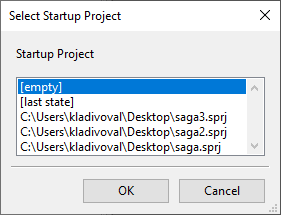
\includegraphics[width=6cm]{../pictures/saga_startup.png} 
\caption[Saga GIS 2.3 startup dialog (source own)]{Saga GIS 2.3 startup dialog (source own)}
\label{fig:saga_startup}
\end{center}
\end{figure}

\subsubsection{Summary}

In the cross-section of all selected GIS software, we can notice that the data hierarchy is quite different. The truth is that two world-famous representatives of GIS software - ArcGIS Pro and QGIS 3 -  have similar data organization into projects. However, in the data hierarchy of the other two commercial software GeoMedia and MapInfo, the term `` project '' does not appear at all. It is therefore good to realize that we may consider this name as a standard for data organization, especially for open-source software, but after looking at commercial software we find out that data organization across software is surprisingly different not only from a technical point of view, but also in terms of different names.

Startup screens appear in some form in all selected commercial software. For GeoMedia, it is a small dialog box whose purpose is purely organizational - choose the GeoWorkspace you will work in. For ArcGIS Pro and MapInfo, startup screens play a more important role. It tries to impress users with both modern design and the services they offer. Similarly, QGIS tries to make contact with the user from the beginning - it refers to news and displays Info Bars (see Fig. \ref{fig:qgis_warning_window}).

The summary corresponding to the questions asked at the beginning of this chapter is contained in the Figures \ref{fig:commercial_software} and \ref{fig:open-source_software}.

\vspace{0.3cm}
\begin{figure}[hbt!] 
\begin{center}
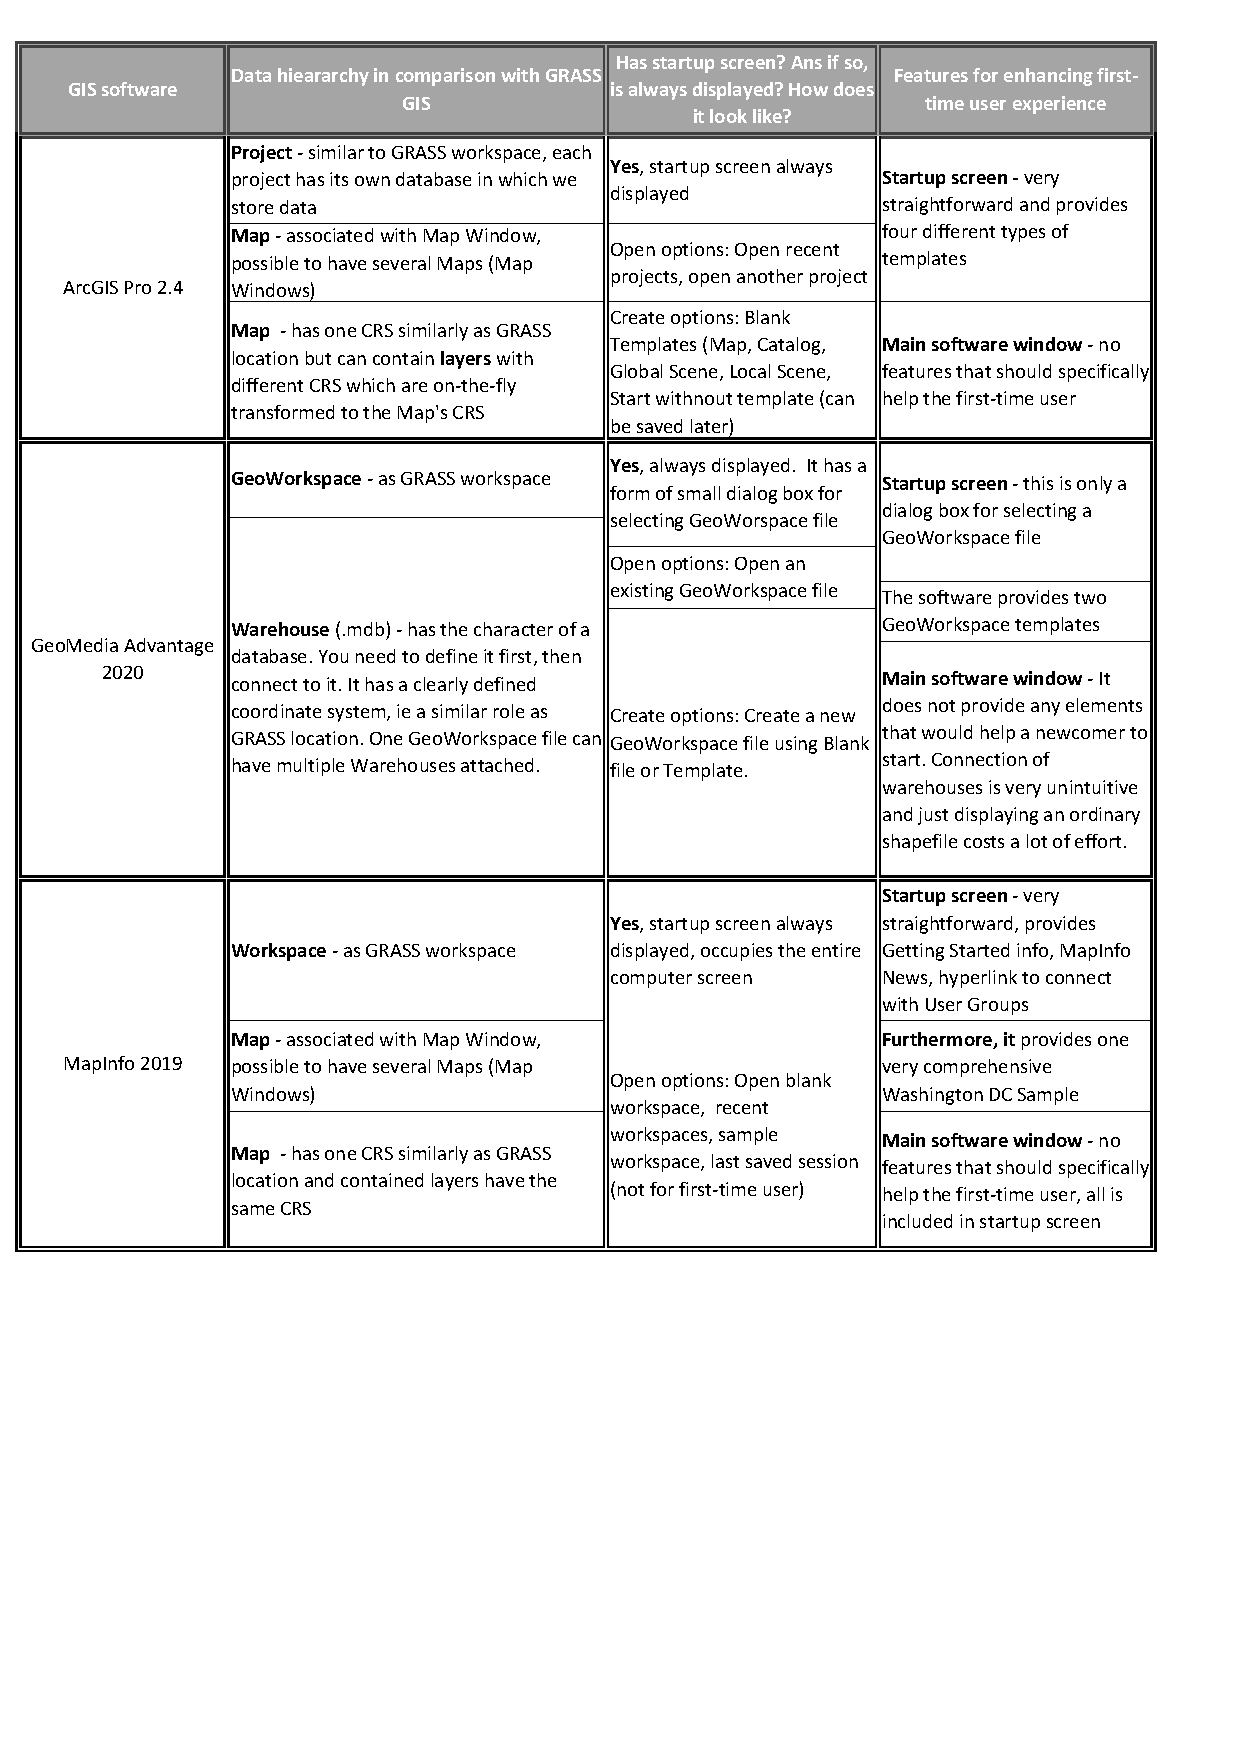
\includegraphics[width=15cm]{../pictures/commercial_software.pdf}
\caption[Analysis of selected commercial software (source own)]{Analysis of selected commercial software (source own)}
\label{fig:commercial_software}
\end{center}
\end{figure}

\vspace{0.3cm}
\begin{figure}[hbt!] 
\begin{center}
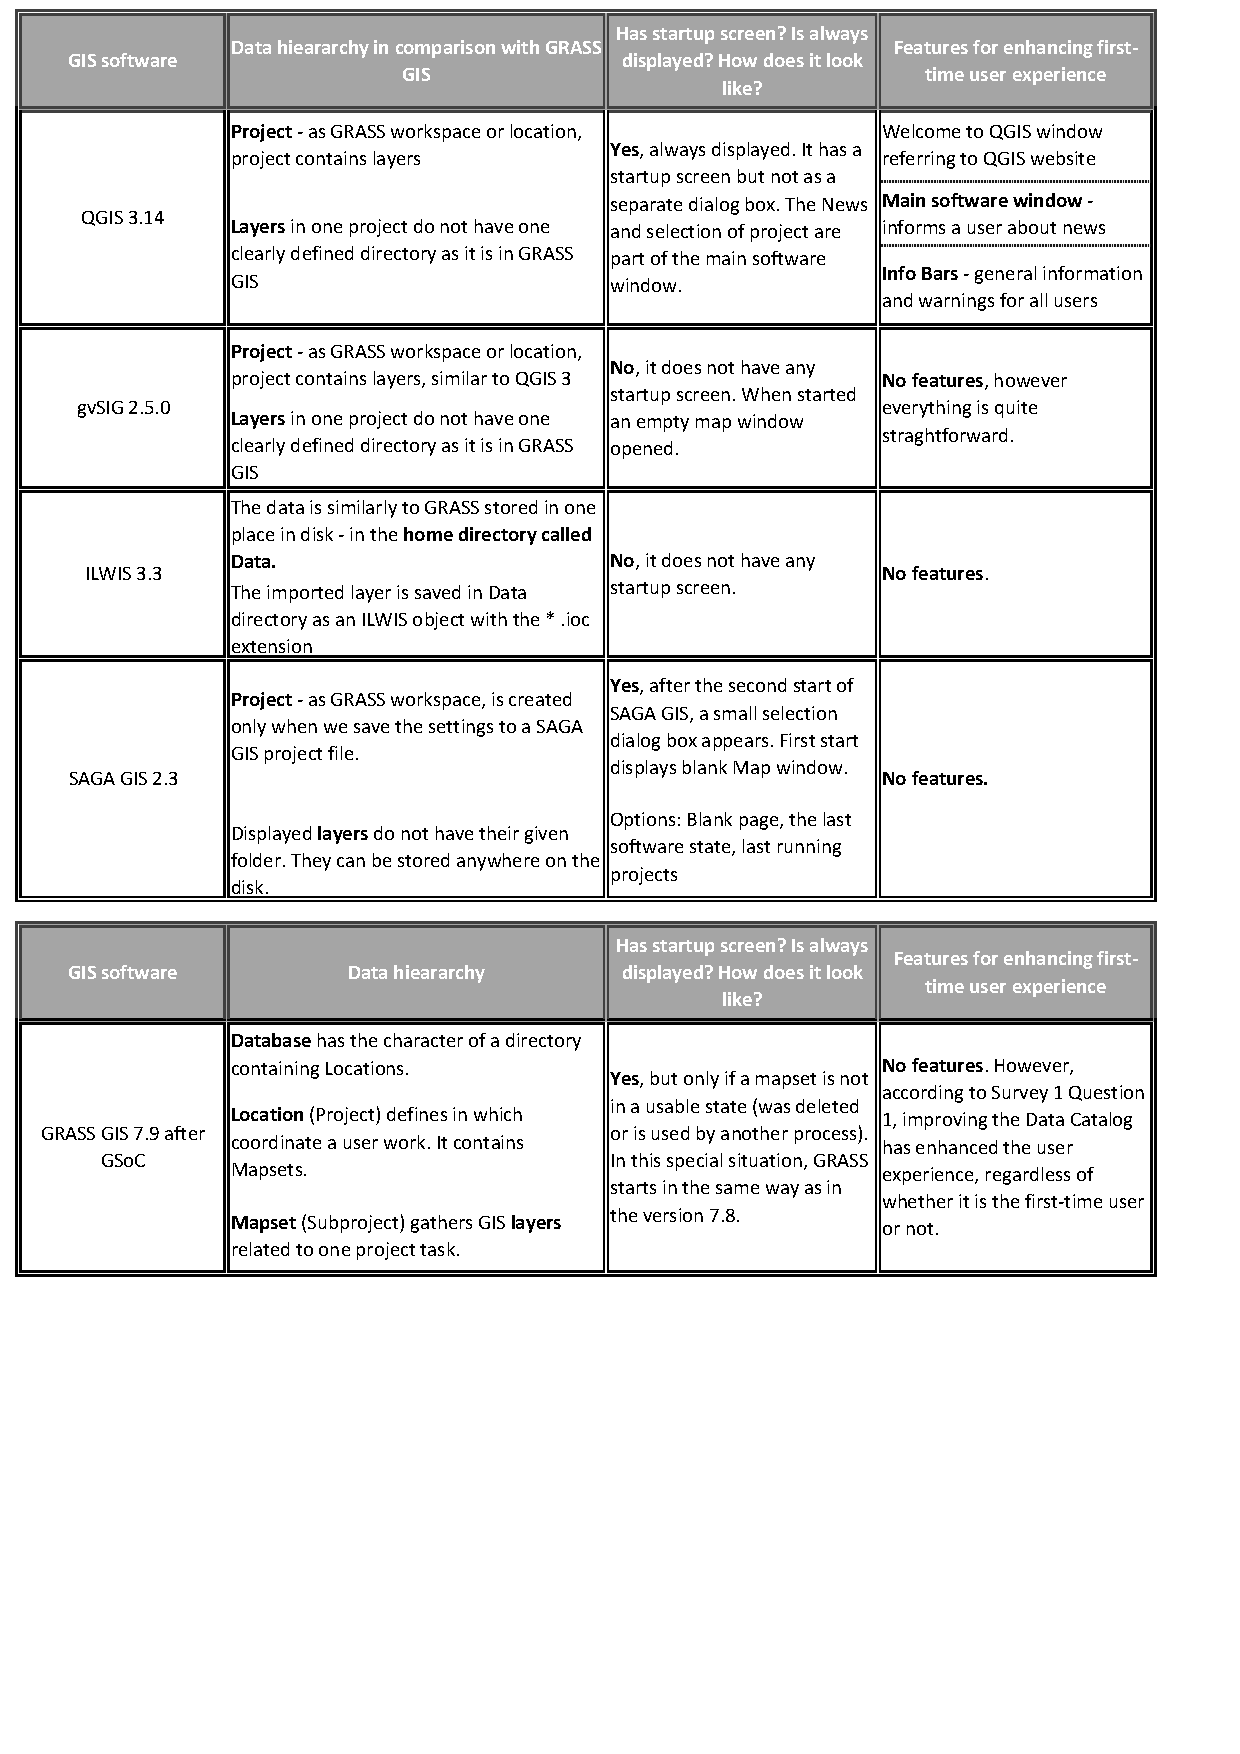
\includegraphics[width=15cm]{../pictures/open-source_software.pdf} 
\caption[Analysis of selected open-source software and GRASS GIS (source own)]{Analysis of selected open-source software and GRASS GIS (source own)}
\label{fig:open-source_software}
\end{center}
\end{figure}

\newpage
It is surprising how much of a difference there can be between commercial GIS software in terms of efforts to enhance the first-time user experience. With the GeoMedia software, the author did not manage to record any effort at all, on the contrary, MapInfo is very generous to its user from the very beginning and uses modern technologies in startup screen, such as videos on YouTube. 

Despite the fact that in some of selected software there is a certain effort to better interact with the initial user, none of them contains any first run wizard incorporated directly in the main software window (as offered by Zoner Photo Studio X, see the next chapter \label{sec:other_software}).

But this is not necessarily wrong. Whether any help at all makes sense and will not be rather counterproductive strongly depends on the complexity of data organization in a particular software. For example, with gvSIG software, there is no startup screen or any other helpful explanation, although it can be assumed that the new user will find his way around without any problems. GeoMedia also lacks any interactive features, however, as data organization is more complex to understand, it is likely to be much more inconvenient start for users.

As known, GRASS GIS went a different way from the beginning. Not only in data organization. The difference between GRASS and other GIS software goes far beyond the startup mechanism or data organization. Let's remember the unique Unix philosophy, where the software consists of a collection of small applications called modules, or the ability to call these modules from the command line.

It is therefore interesting to note that the comparison of GRASS GIS with other GIS software does not provide significant inspiration for other implementations associated with the improvement of the startup mechanism, which requires (and probably deserves) a completely unique solution, the implementation of which has already started at GSoC. However, the comparison offers an interesting look at this topic, which is not talked about much, but certainly has a big impact on the whole software. The evidence may be, after all, the problematic startup screen in versions before GSoC.

However, it is not necessary to look for inspiration only in GIS software, because how the software interacts with the first-time user is a completely general thingr that we can observe in all types of software. In the next chapter, the author tried to highlight several interesting cases of startup mechanisms involving user interaction. These are software that the author either uses herself or received a tip from the survey number 2.


\newpage
\vspace*{-1cm} 
\subsection{Interesting solutions from other software}

\noindent \textit{\color{red}Dokončit!}

\noindent \textbf{Zoner Photo Studio X} \\

\noindent After the initial login and launching the main software window, a short first run wizard will appear and can be skipped. The guide consists of four parts. The first section introduces the main tabs on the left side of the software window called the Navigator and also explains the Catalog tab, which provides quick access to photos. The following are two pages of a guide describing photo thumbnails and zooming. The last page of the wizard lists the right toolbar and the three individual modules - Manager, Develop and Editor. The main software components described in the wizard are always marked with a blue frame and the individual information windows are assigned to a particular part by arrows. The wizard is not only at the beginning, but also when using the above-mentioned modules for the first time.

Images are managed in the Catalog, which has a tree structure. We edit the image, save it, and if we turn off the Zoner software and run it a second time, it starts up in the last opened file. If the last used file is deleted, the software is launched in the Manager tab in the last opened folder, where another image can be selected for editing or we can simply click to another folder and open or create another image. There is a native image format of Zoner Photo Studio X with extension * .zps, however, firstly, traditional formats such as * .jpg, * .png, * .tif, * .gif etc. are offered to us.

\vspace{0.3cm}
\begin{figure}[hbt!] 
\begin{center}
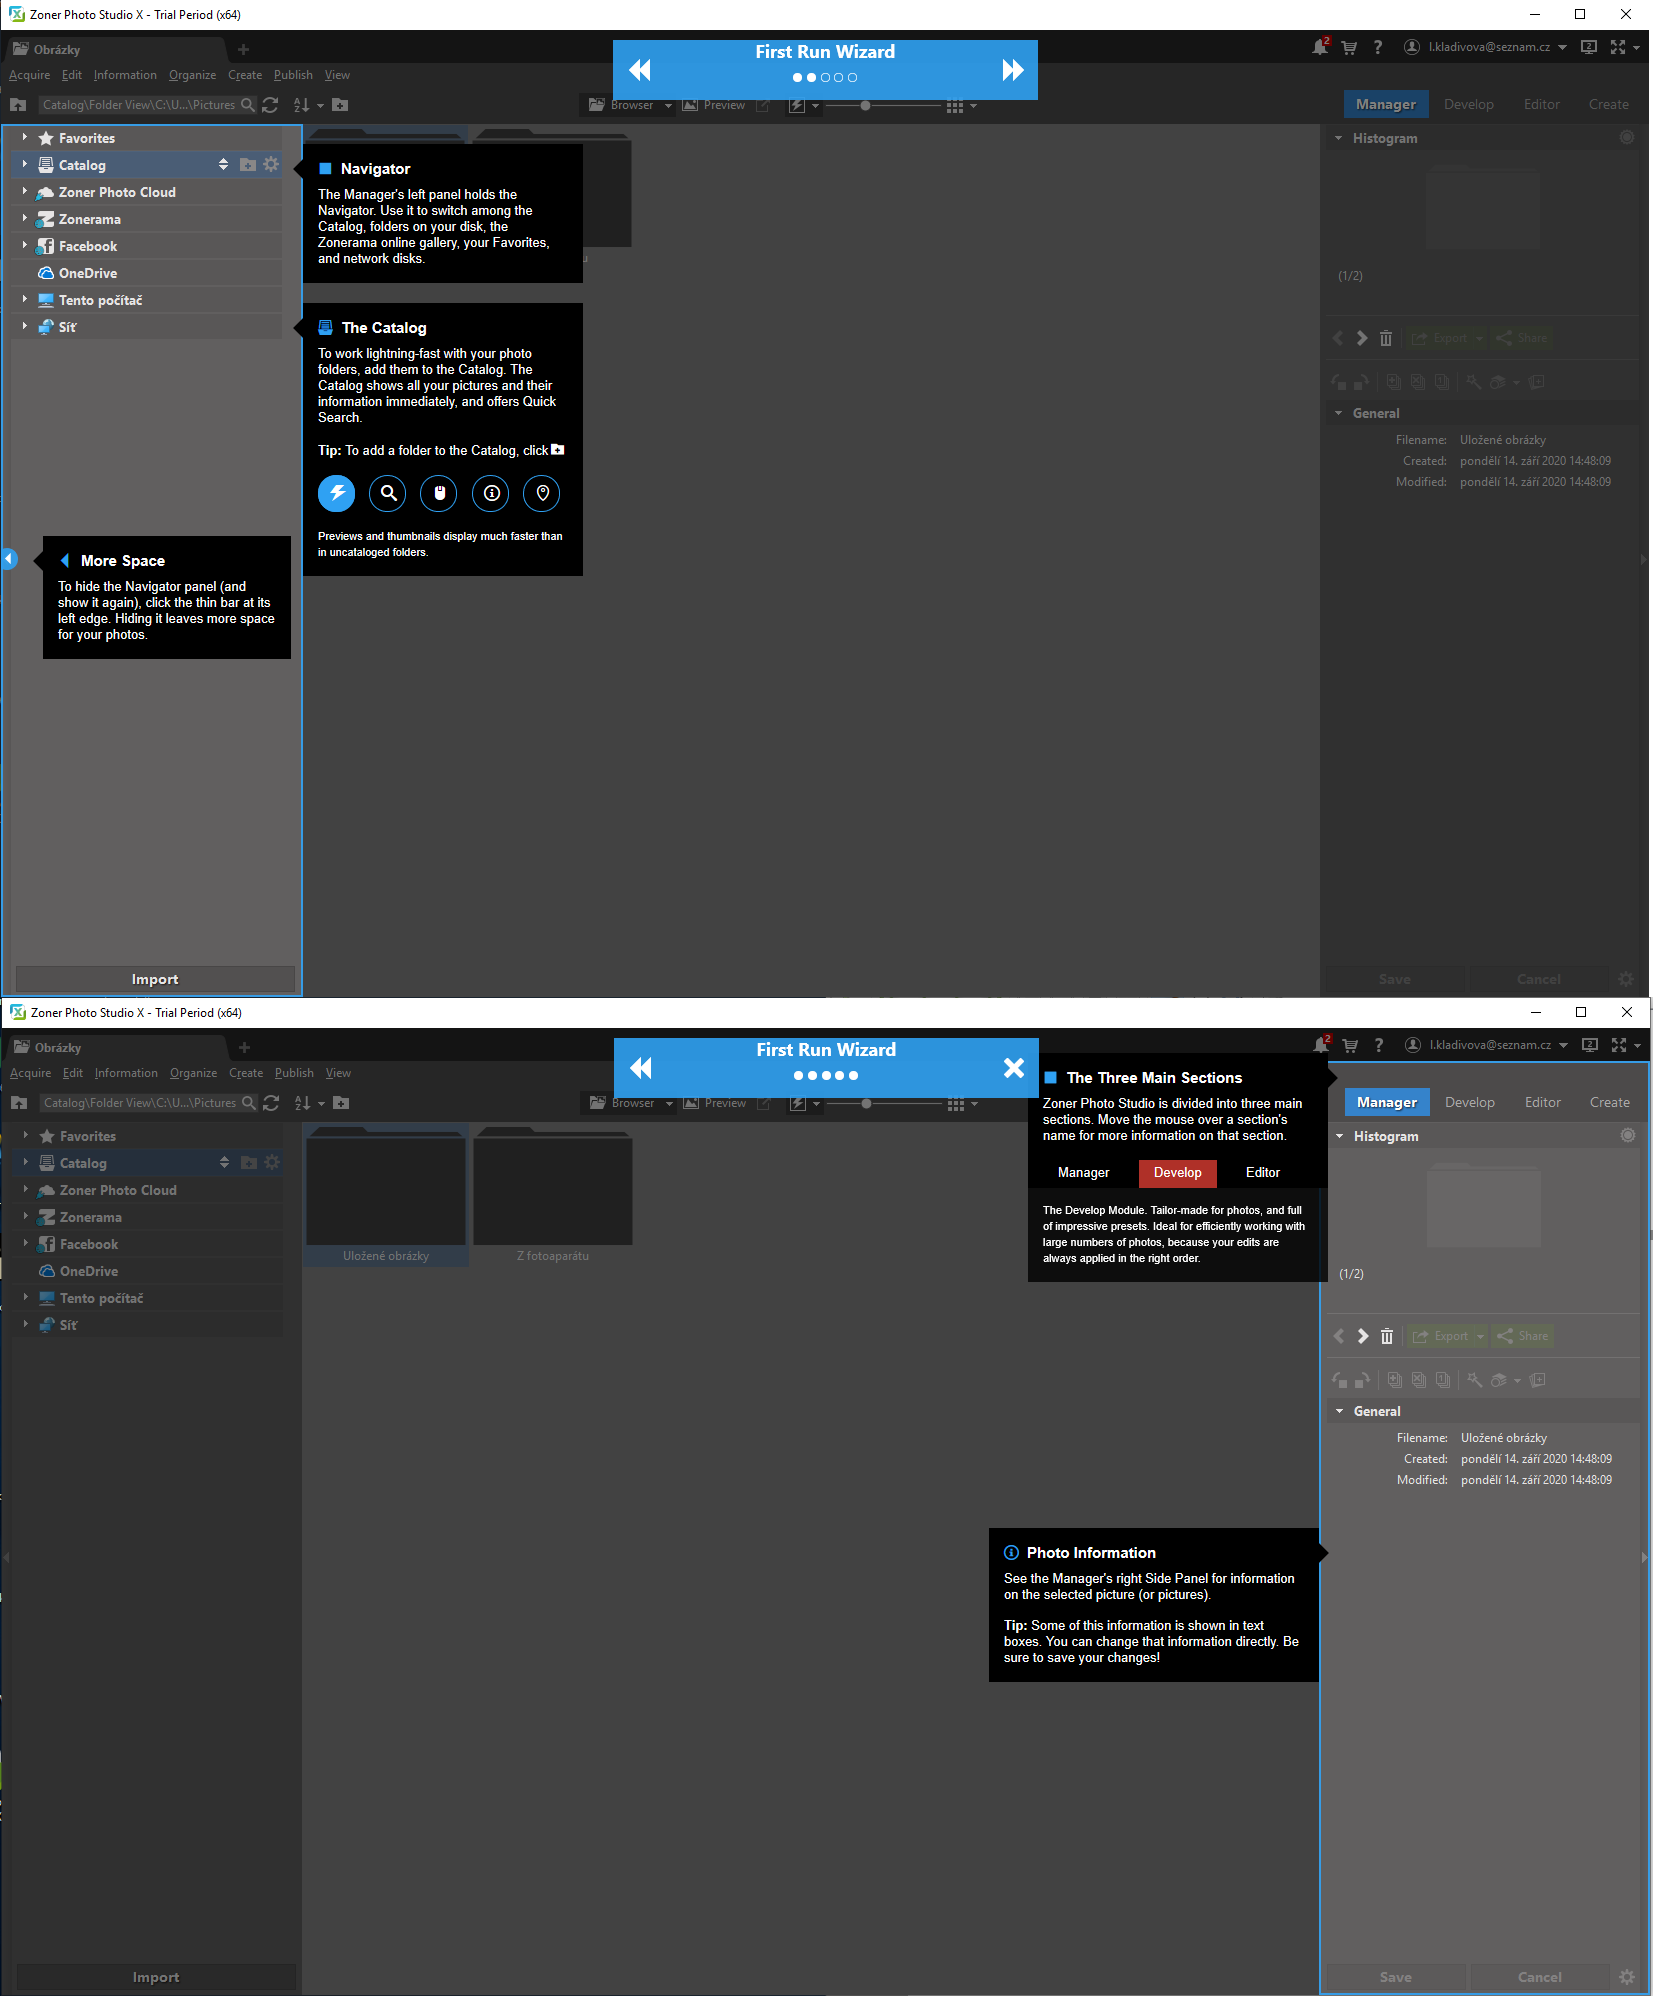
\includegraphics[width=15cm]{../pictures/zoner.png} 
\caption[First run wizard in Zoner Photo Studio X]{First run wizard in Zoner Photo Studio X}
\label{fig:zoner}
\end{center}
\end{figure}

\newpage
\vspace*{-1cm}
\subsection{Summary}


%% -------<<< Chapter 4:Analýzy výsledků prvních dvou průzkumů>>>-------\\%%%%%%%%%%%%%%%%%%%%%%%%%%%%%%%%%%%%


\newpage
\vspace*{-1cm}
\section{Analýzy výsledků prvních dvou průzkumů}

\noindent Hlavní částí této práce je několik testů a průzkumů, které se obecně řečeno, snaží získat preference uživatelů v souvislosti se směřováním dalšího vývoje GRASS GIS. Lze říci, že provedené testy a průzkumy nejsou zaměřeny pouze na otázku first-time uživatele a proto jejich výsledky (návrhy na vylepšení) často výrazně přesahují rámec implementací provedených v této práci. Implementační část této práce se totiž výhradně soustředí na to, jak vylepšit first-time user experience. 

\subsection{Research: Help improve GRASS GIS startup mechanism and Data Catalog}

    Q1: velké většině lidí se libí, jak jsme to změnili, je dokonce 14 z 52 odpovědí na 100 bodech
    Můžeš z toho udělat histogram? Ten počet bins pro histogram můžeš založit na originálním SUS. Průměr 70 mi přijde menší nadšení než jsem čekal. 
    
    myslím, že podle boxplotu a histogramu už se dá usoudit, že se valné většině stav po GSoC líbí. 
Mimochodem, jeden člověk hodnotil tuto otázku nulou, tak mě zajímalo, jak reagoval v jiných otázkách (respondent \#22). No a zjistila jsem, že byl celkově docela negativní. Asi nějaký člověk, co nemá rád změny. :-D.... 


    Q2: lidi navrhují modernized version of startup screen celkem v přesile

    -- otázka je, jak by měla vypadat. Zatím se mi asi nejvíc líbí ta varianta, kdy by nabízela dříve uložené workspacy
    -- inspirovala bych se softwarem MapInfo, startup tohoto softwaru posílám v příloze, samozřejmě by to nemuselo být takto složitý
    -- nebo něco podobného má SAGA, rovněž příloha
    -- demolokaci bych určitě zobrazovala s mapou, někdo to zmínil v tom průzkumu a přítel mi to taky několikrát zdůraznil -Jo, to já taky! Pro kohokoliv, kdo nezná GISy, je nějaká mapa nutností. Anička připomíná, že Blender (3D modelování) zobrazuje kostku.
    Myslíš na startup screen pro každého?
    
    Neni mi jasne jestli všichni pochopili kontext. Ze samotné otázky není jasné, že je to v kontextu, kdy startup screen vůbec nebude vidět v ostatních případech. Některé "own ideas" to podle mne silně naznačují.

Jinak obecně tohle jako neočekávaný a nejasný výsledek můžeš zkusit vysvětlit pomocí těch rozhovorů, kde se můžeš zeptat na detaily.

Nějaká startup screen bude potřeba pokud zachováme --gtext, takže ten scénář s jednoduchou backup startup screen (souřasný g.gui.datacatalog) by neměl být takový problém implementovat.

Ano, v číslech 6 a 8 to pravděpodobně nepochopili ... :-( ale jinak vesměs navrhují jednoduchý dialog (warning message), který by měl na výběr nějaké možnosti, co dál, viz co jsem psala v minulém emailu. Myslím, že by se to dalo řešit i jednodušeji než vytvářením dalšího Data Catalogu. Navíc ani nikdo z respondentů nic takového nenavrhuje, vesměs se jedná o warning messages. Mohla by to být nakonec i taková úplně jednoduchá startup screen podle Moritzova návrhu. Ale asi bych ji zobrazovala opravdu jen tehdy, kdy "last used mapset is not in usable state". Ikdyby třeba lidi něchtěli pokračovat v posledně otevřeným mapsetu, můžou se pak v Data Catalogu jednoduše přepnout jinam. Nebo si mohou uložit workspace a ten si pak otevřít. Co myslíte?


    Q3: přidání více databází nemá zas takový úspěch, jak bych si myslela, naopak management iconky mají velký úspěch
    
    Rozdíly nevypadají signifikantně, ale hlavně já jsem trochu zmaten. 1 = most useful, ale to score je obráceně?

Rozhodně je to přehozená stupnice od těch modified SUS, takže možná došlo k zmatení. Správné by asi bylo nejprve udělat usability test na to survey...

 Tady došlo trošku ke zmatení od Survey Monkey, kdy tyto ranking odpovědi vyhodnocují na základě Score, viz https://help.surveymonkey.com/…ion . Je to vážený průměr, kdy se každému pořadí stanoví váha (1. prvek na váhu 7 v našem případě). Myslím si, že lidé pochopili dobře, že most useful = 1, kontrolovala jsem i konkrétní odpovědi a nevšimla jsem si, že by někdo nápadně zaměnil pořadí. Posílám ještě podrobnější statistiku.


    Q4: tam je hodně zajímavý návrhů, jaké funkce přidat. Vypíchla bych: Drag and drop vector/raster layers into map window, Zoom to layer in context menu,  the EPSG code next to location name, delete more than one layer via context menu, cloning location, space-time datasets listed too. Je jich ale mnohem víc.
    Také tam hodně informací o celém GUI ne úplně souvisejících s tvojí prací, ale poučných. Mnoho lidí nemůže najít WMS/basemaps nebo jim to přijde moc těžké a považují to za důležitou funkcionalitu ve vztahu k datům. Hodně lidí mluví o tom, co je v Display, což naznačuje, že bude/je problém pro uživatele rozlišit funkci tabů Data a Display.
  
 Tuto otázku jsem koncipovala dost obecně, což myslím vedlo k tomu, že lidi často nenavrhovali věci k Data Catalogu, ale spíše obecně ke GUI.... No, nevím, jestli to byla zrovna správná cesta :-D... nicméně zaznělo i spoustu věcí mimo Data Catalog. Pokusila jsem se odpovědi roztřídit.

    Q5: Tady se větsina shodla na přidání dalších funkcí do context menu anebo do obou (jak context menu tak management icons)
Hádám, že rozdíl To management icons a To both není signifikantní. Takže ta odpověď je context menu. I don't think any features should be added... dostalo překvapivě hodně hlasů.
Jop, context menu, a souhlasím, to s tím místem je zajímavý. Odpovědělo to 7 lidí, z toho 1 byl ten respondent \#22, ale ostatní \#1, \#4, \#17, \#27, \#36, \#52, jsou uživatelé, kterým se stav po GSoC velmi líbí... Asi se bojí, aby to celkově nebylo moc přeplácané, jiné vysvětlení mě nenapadá. S tím souvisí, že v otázce č. 4  zaznělo sice hodně možností, co přidat do Data Catalogu, ale nikdo nezmínil nic více komplexního jako třeba Import Dat. Ty vylepšení se týkají spíše správy datové hiearchie.

    Q6: Tohle je docela překvapité. Nevypadá to, že lidé využívali startování GRASSu skrze ikonku často. 54 procent jako odpověď mi přijde dost málo. Asi jsou zvyklý na CLI.
    Opět, histogram je potřeba na lepší interpretaci. Medián by mohl být dobrý na ano/ne rozhodnutí. Ale jinak je to celkem očekávané.
    Ta alternativa není (jen) CLI, ale (hlavně) to jak se GRASS GIS startuje teď, tedy výběr mapsetu (přes GUI nebo nově last used automaticky).
    Tyhle odpovědi jsou takové nejednoznačné. Mám z toho podobný pocit jako ty Vašku, totiž, že jsou teď další alternativy, jak GRASS startovat. Přemýšlela jsem taky nad tím, jestli třeba v QGISu tuhle možnost využívám a došlo mi, že ani moc ne a to QGIS používám v práci celkem často. Vždycky si ho spustím (v tu chvíli ještě ani nepřemýšlím, jak se konkrétní projekt, který chci jmenuje), pak ho hledám mezi posledně zavřenými projekty, ale někdy se stejně dostanu do situace, že otevřu prázdný projekt.... Nevím, jak to mají ostatní, ale jako první prostě většinou otevírám software a až pak přemýšlím, kde mám data, které chci otevřít. Jak to máte vy?
Takže tohle je velká otázka, zda implementovat. Zase pravda je, že tomu, kdo to nechce to nijak neublíží, prostě to používat nebude (ani si toho třeba nevšimne, že to jde) a ten kdo to bude chtít používat, to využije. Z tohohle pohledu by dávalo smysl to implementovat. Co si myslíte?

\newpage
\vspace*{-1cm}
\subsection{Research: Help create a better first-time user experience in GRASS GIS}

    Q1: tady mi přišel zajímavý druhý komentář. Mám totiž pořád trochu strach z těch Info Bars v Demolokaci, jelikož si myslím, že aby to za něco stálo, musely by obsahovat více informací. Dává tedy mnohem větší smysl, tyto informace dát někam jinam, ale dobře na ně odkázat. To souvisí i s mnoha dalšími odpovědmi, kde lidé navrhují třeba krátká videa, případně dobrou dokumentaci. Možná by ty Info bars mohli obsahovat jenom hodně kraťoučkou instruktáž a pak rovnou hyperlink, na nějaké video (případně dokumentaci).
    S tím souvisí i to, že by možná stálo zato udělat tu hodně jednoduchou startup screen. Bylo by to opravdu jen o tom nabídnout demolokaci, případně prázdnou lokaci a potom nabízet posledně uložené workspace, případně Last Saved Mapset, jako je to nyní. A pak by tam byly odkazy na video a na tutoriál, na stránky GRASSu, novinky apod. To ovšem neznamená, že by se nedali zrealizovat i ty Info Bars. Ty by byly vztaženy pouze a jenom k otevřené demolokaci.
    
    Ano, do těch info bars se toho moc nevejde, takže nějaké Learn more bude potřeba.

Jinak to Yes but č. 2 my přijede nejužitečnější.

Pro všechny? Přemýšlej kdy a jak ji zobrazit? Jako QGIS místo mapy, jako v 7.8 nebo jako ve starším návrhu Proposal B1 (Moritz) : Open into a predefined lat-long location but give information message?

https://trac.osgeo.org/grass/wiki/wxGUIDevelopment/New\_Startup\#ProposalB1Moritz:Openintoapredefinedlat-longlocationbutgiveinformationmessage

        To ovšem neznamená, že by se nedali zrealizovat i ty Info Bars. Ty by byly vztaženy pouze a jenom k otevřené demolokaci.

Souhlas, to je nezávislé.

 Tady máš pravdu, že vlastně to yes, but znamená spíš no, because :-) . Takže to vychází zhruba 69.5 \% pro a 30.5 \% proti.



    Q2: Lidem se líbí oba nápady, jak Info Bars jak First Run Wizard
    
    To jsme tak nějak čekali. Když zkombinuješ obě No a možná pár odmítavých Yes, but možná dostaneš docela dost Ne, což je také zajímavé, protože to není pak tak jasné. I jen z Yes, but pro Q1 to vypadá, že musíme být opatrní.
    Tady můžeme tvrdit to podobné, po spojení ano a ne mi vychází 74 \% pro a 26\% proti. 

    Q3: líbí se mi třetí komentář - immediately show map at first startup -- provide links to tutorial videos, nebo zajímavá je taky odpověď 13, a pak hodně lidí navrhuje single layout
    
    Tady by to chtělo vzít ty odpovědi a nějak je klasifikovat/roztřídit podle toho o čem mluví a/nebo, co by to mohlo vyřešit. To platí i pro ostatní open ended questions, ale zde snad nejvíce. 1) Requires removing db/loc/mapset structure 2) Already exists (so perhaps hard to find or otherwise unknown) 3) Asks for more doc or info on db/loc/mapset 4) Asks for videos ...

Když to takhle zpracuješ, tak to možná bude nejužitečnější z tohodle survey.

Trochu zamotaný 14 (terminologie) je něco, o čem jsem hodně přemýšlel. Ten vztah mezi popisem G algs v QGISu a v samotném GRASSu, co konkrétně zminuje ten člověk, je něco, co by se mělo řešit přímo v GRASSu. QGIS má svoje vlastní popisy všech věcí v GRASSu - a ty by mohly být v GRASSu jako v nějakém obecném GIS názvosloví. Ale to jen tak mimochodem.

Ale 14 souvisí s 1, Q1 1, Q4 1: Kdyby se db/location/mapset jmenovali nějak jinak (nebo byly jinak prezentovány), slovo old by nebylo součástí kritiky. "Je koncept databáze old pro PostgreSQL či Oracle?" To je samozřejmě absurdní otázka. Třeba CLI byla vnímána jako negativní, ale nyní, alespoň mimo GIS, CLI teď jen roste (stejně jako v (mnohem) menším roste LaTeX). Ta klasifikace by právě měla vytáhnout tyhle souvislosti (i když netvrdím, že musíš jít do všech detailů, jen co je praktické pro tvoje programování).

Tady mi připadá, že respondent 13 (v celkovém dokumentu, který taky posílám je to respondent 34) by chtěl prostě jen lepší dokumentaci metod, které se chystá použít. Myslím, že nic takového, co on navrhuje GRASS nemá, nebo má? U otázky Q5 dal description of main tabs až na poslední místo.
U respondentů 20 a 21 (respektive 27, 26) těžko říct, 26 dal Main tabs až na poslední místo, 27 na první místo. Ale asi záložku Modules úplně nepochopili
 
 
    Q4: často zmiňují QGIS... podívám se nicméně i na ty další, co zmiňují
    
    Any idea what "really like (old) QGIS simple UI" means?

Jinak já to vidím tak, že to nemusí být stejné jako QGIS. Ideálně to bude nejlepší řešení pro GRASS GIS, viz 42 v Q3.
Naprostý souhlas. Ale překvapilo mě, že vlastně skoro všichni napsali QGIS. Podívám se ještě na ten Discord a Slack. Měly by to být nějaké chatovací prostředky pro týmy, něco jako modernější Jabber..

    Q5: tady je to hodně vyrovnaný, no nicméně, nějaká rada, jak začít v demolokaci určitě měla být. Vím, že přítel měl třeba problém, že ho nenapadlo si v demolokaci založit novou lokaci a všechno by to házel do té demo... Takže něco jako, teď si založ novou lokaci a tady naimportuj data, by bylo dobré. To bych asi dala do těch Info Bars. Vysvětlení grassdb, lokace a mapsetu mi připadá moc dlouhé, na to by mohli být jenom odkazy třeba na to video. 
    
    Souhlas, ale z Q3 je vidět, že třeba "Description of main tabs (Data, Display, Modules..." by také bylo důležité. Ale i ty druhé dvě jsou vidět v Q3 a měly by být součástí té klasifikace pro Q3.
    Main tabs v otázce Q5 dala pětina respondentů na první místo, takže souhlasím, že můžeme dedukovat, že s tím mají lidé problémy.

Můžeš se podívat na jednotlivé respondenty? Co zde odpověděli 13, 20 a 21?
    
    
\newpage
\vspace*{-1cm}
\section{How to create a better GRASS GIS startup mechanism: Proposal}
\noindent
\large
At this special moment, I suggest displaying a warning message and demolocation in the background (according to Moritz's B1 proposal \footnote{\url{https://trac.osgeo.org/grass/wiki/wxGUIDevelopment/New\_Startup\#Changeparadigm}}. There would be two types of messages that are displayed according to the situation. In other situations, where it is possible to start the last usable mapset, we may go straight to the Layer Manager and Map Display (we will not display the startup screen under any circumstances). \\

\noindent The first situation is when the last used mapset is is use. At this point, the question message  "Last Used Mapset is in use", similar to the situation already happening in Data Catalog when switching to a mapset in use (Figure \ref{fig:data_catalog_switch_new_2}), would be displayed.

However, the choices would be:
\begin{itemize}
\item Switch to selected mapset
\end{itemize}
\begin{itemize}
\item Switch to demolocation
\end{itemize}
\begin{itemize}
\item Quit
\end{itemize}


\noindent The second is when the last used mapset has been deleted, or the entire grass database or location has been deleted. At this point, this would be a "Last used mapset was not found" warning message.
Then it would give a user a straight choice of Switch to demolocation, where a person would simply open the database he needs from the Data Catalog and switch to desired mapset. 
It should switch to demolocation without info bars, as this will not be for first-time users.\\

\noindent Several interesting ideas for improving the Data Catalog were suggested in the surveys:
\begin{itemize}
\item Create location according to projection of given GIS file
\end{itemize}

\begin{itemize}
\item More friendly layer coloring accessible from layer tree
\end{itemize}

\begin{itemize}
\item Easily move items between mapsets/locations
\end{itemize}

\begin{itemize}
\item The EPSG code in parenthesis just after the location name
\end{itemize}

\begin{itemize}
\item Delete more than one layer via context menu
\end{itemize}

\begin{itemize}
\item Cloning location
\end{itemize}

\begin{itemize}
\item Location metadata (which CRS, number of mapsets in use, with a different user)
\end{itemize}

\begin{itemize}
\item STDS listed in data catalog and when clicking on the STDS name, see maps registered within them
\end{itemize}

\begin{itemize}
\item Saved workspaces visible somewhere in the data catalog
\end{itemize}

\newpage
\vspace*{-1cm}
\section{How to enhance first-time user experience: Solution}
\noindent
\large

A world map would be displayed automatically at startup.
Info Bars (inspired by QGIS) have been quite successful with users. However, there is some uncertainty and caution in creating a first-time mode. Some people are afraid that the newly created mode will be complicated and rather annoying.
I suggest to create light yellow Info Bars that only better develop the demolocation, which will be automatically offered to every new user.\\

\noindent I would suggest to include in these info bars brief explanations of how to get started (it's not long), a small info bar might also be for each of the tabs (Display, Modules, Console, Python, Map Display). The implementation would be as follows:

\vspace{0.3cm}
\begin{figure}[hbt!] 
\begin{center}
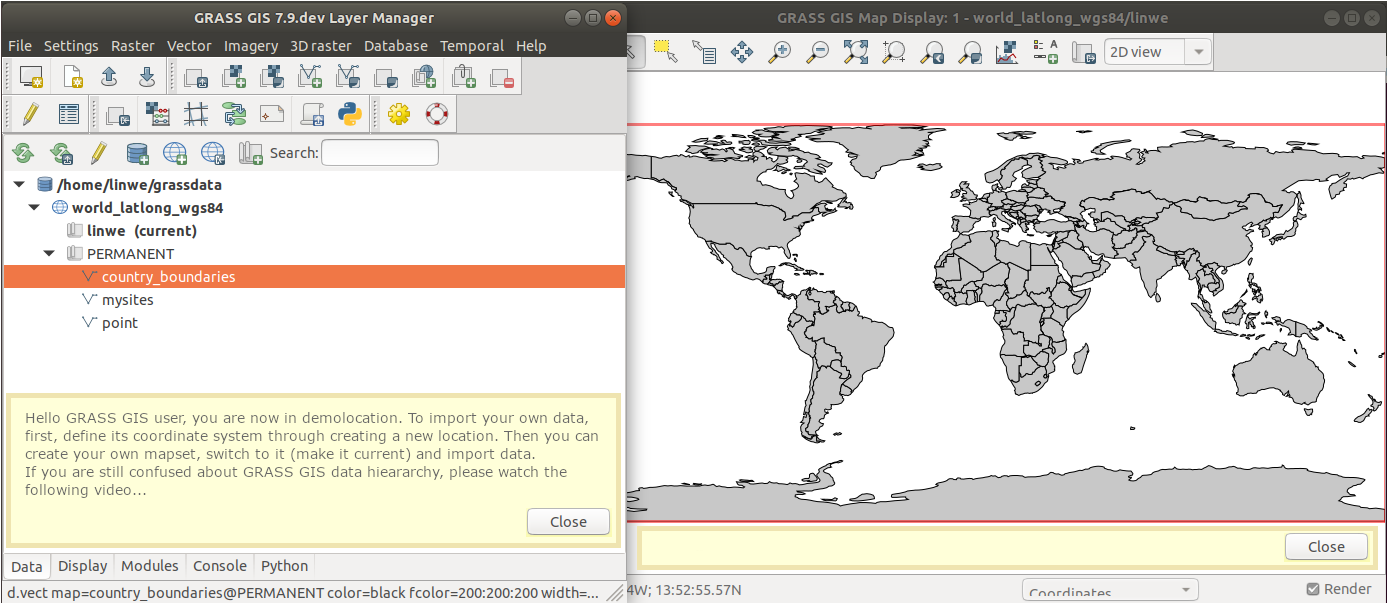
\includegraphics[width=15cm]{../pictures/infobars.png} 
\caption[proposal for future implementation of Info Bars]{proposal for future implementation of Info Bars (source: own)}
\label{fig:infobars}
\end{center}
\end{figure}

\noindent For further explanation (e.g. of data hierarchy), there would be a link to a video on YouTube, or to the documentation.

\newpage
\section{Other improvements}

There are also some important things about the Map Window in particular:

\begin{itemize}
\item	Drag ad drop vector/raster layers into map window
\end{itemize}

\begin{itemize}
\item	Zoom capability with mouse without messing up the window

Related abbreviations are related to this:
\begin{enumerate}
\item mouse wheel zoom in and zoom out (or CTRL + wheel) ideally to zoom in and out toward / away from the current cursor position

\item CTRL + mouse - zoom using box (or SHIFT + mouse)
\item right button - context menu for the selected vector features
\item move the map without having to select the icon from the top bar
e.g. only via CTRL + mouse (or SHIFT + mouse)

\end{enumerate}
\end{itemize}

And other topics from surveys:

\begin{itemize}
\item Easier process to access WMS/WFS (add WMS button)
\end{itemize}

\begin{itemize}
\item Icon for region settings
\end{itemize}

\begin{itemize}
\item Create association of workspace file
\end{itemize}

\begin{itemize}
\item Explain regions and mapsets and how it will affect your session, data import/export options
\end{itemize}

\begin{itemize}
\item Put all GRASS into a single window
\end{itemize}

\begin{itemize}
\item Undo button
\end{itemize}

\begin{itemize}
\item What about command line options? Are they still available?
\end{itemize}

\newpage
\vspace*{-1cm}
\fancyhead[RE, RO]{\fancyplain{}{\small \sl{Used technologies}}}
\section{Used technologies}
\noindent
\large

\noindent This chapter briefly presents GRASS GIS, a Geographic Information System (GIS) technology built for vector and raster geospatial data management, geoprocessing, spatial modelling and visualization, from both historical and technical point of view. Furthermore, it describes the main programming technology used for a new startup GUI implementation, called wxPython.

\subsection{GRASS GIS}
\noindent
\large

\noindent GRASS (Geographic Resources Analysis Support System) is a cross-platform desktop geographic information system (GIS) designed to work with geographic 2D/3D raster and vector data, image records, both using the command line and graphical user interface (GUI). Besides, it enables the production of high-quality graphic outputs, spatio-temporal modeling, data visualization, or connection to spatial databases.

The development of the GRASS GIS system was started by the research laboratories of the US Army Engineer Engineer in 1982, later got into the academic sphere and today it is also used in the commercial sphere. It is open-source software published under the GNU GPL general license and managed and developed under the OSGeo organization. Important users of the GRASS system include, for example, NASA or NOAA.

The power of software stems mainly from its Unix philosophy, where the software itself consists of a collection of more than 500 applications called modules. Each of these modules has only one task to perform, and the real power of the software comes when the various of these modules begin to chain together, allowing the user to create even very complex applications. Most of these modules are written in C, but above the whole system, PyGRASS as an object-oriented Python Application Programming Interface (API) stands, which hides the complexity of GRASS and provides access to the capability of the C- API of GRASS for geo-scientists that are not familiar with C.

Nowadays, most main changes take place in the python programming language, which also applies to the GUI, which uses the wxPython extension. The software has been developing since January 2020 on GitHub, a web service that supports development using the Git versioning tool. This principle makes working on code much clearer. It stores the history of work, ensures stylistic consistency using the flake8 command-line utility, and also allows the creation of Issues, which can have the character of errors and various improvements. Then these issues are usually proposed for changes (so-called pull requests), which users discuss. Therefore, GitHub partly works as a social network, which can support the creativity and enthusiasm of developers.

At this point, I would like to mention that besides improving the GRASS GIS startup mechanism, in summer 2020 the community presented a new website on the occasion of its 37th birthday (stable version 7.8.) which offers a curated list of tutorials in different languages and links to videos.

\vspace{0.3cm}
\begin{figure}[hbt!]
\begin{center}

\includegraphics[width=15cm]{../pictures/grass_gis.png} 
\caption[New GRASS website's layout]{New GRASS website's layout (source: \url{https://grass.osgeo.org)}}
\label{fig:grass_gis}
\end{center}
\end{figure}

\subsection{wxPython}
\noindent
\large

\noindent This open-source toolkit allows Python programmers to create a graphical user interface. We can import it to a script file as a package that wraps the GUI components of the popular wxWidgets cross-platform C++ library established in 1992 at the Artificial Intelligence Applications Institute at University of Edinburgh. There are a number of other graphical user interface (GUI) packages for Python, for example, the Tkinter package is also very popular.

wxPython is a cross-platform toolkit which means that the same program can be run on multiple platforms without modification. Currently, supported platforms are Windows, macOS, Linux, or other Unix-like systems. The resulting design on each platform can be a bit different as we can also notice when using GRASS GIS on different systems. 


%% -------<<< Chapter 3: Implementation>>>-------\\%%%%%%%%%%%%%%%%%%%%%%%%%%%%%%%%%%%%
\newpage
\vspace*{-1cm}
\fancyhead[RE, RO]{\fancyplain{}{\small \sl{Implementation}}}
\section{Implementation}
\noindent
\large

%% -------<<< Chapter: Discussion >>>-------\\%%%%%%%%%%%%%%%%%%%%%%%%%%%%%%%%%%%%
\newpage
\vspace*{-1cm}
\fancyhead[RE, RO]{\fancyplain{}{\small \sl{Discussion}}}
\section*{Discussion}
\addcontentsline{toc}{section}{Discussion}
\noindent
\large

%% -------<<< Chapter: Conclusion >>>-------\\%%%%%%%%%%%%%%%%%%%%%%%%%%%%%%%%%%%%
\newpage
\vspace*{-1cm}
\fancyhead[RE, RO]{\fancyplain{}{\small \sl{Conclusion}}}
\section*{Conclusion}
\addcontentsline{toc}{section}{Conclusion}
\noindent
\large

%% -------<<< Chapter: List of abbreviations >>>-------\\%%%%%%%%%%%%%%%%%%%%%%%%%%%%%%%%%%%%
\newpage
\vspace*{-1cm}
\fancyhead[RE, RO]{\fancyplain{}{\small \sl{List of abbreviations}}}
\section*{List of abbreviations}
\addcontentsline{toc}{section}{List of abbreviations}
\noindent
\large


%% -------<<< LITERATURA >>>-------\\%%%%%%%%%%%%%%%%%%%%%%%%%%%%%%%%%%%%%%%
\newpage
\vspace*{-6ex}
\renewcommand{\refname}{Bibliography} 
\addcontentsline{toc}{section}{Bibliography}
\fancyhead[RE, RO]{\fancyplain{}{\small \sl{Bibliography}}}
	\selectlanguage{english}
	\bibliographystyle{plain}
	\bibliography{bibliography}

\noindent
\large

https://trac.osgeo.org/grass/wiki/wxGUIDevelopment/New\_Startup\#PragueRoadmap \\

Zambelli, P.; Gebbert, S.; Ciolli, M. Pygrass: An Object Oriented Python Application Programming Interface (API) for Geographic Resources Analysis Support System (GRASS) Geographic Information System (GIS). ISPRS Int. J. Geo-Inf. 2013, 2, 201-219. \\

Predicting Database Requirements for Geographic Information Systems in the Year 2000: Long-Term Design Issues for GRASS. August 1992.\\

Goran, W.D., Dvorak, W.E., Van Warren, L. and Webster, R.D., 1983, Fort Hood Geographic Information System: Pilot System Development and User Instructions, Technical Report N-154, USA Construction Engineering Research Laboratory, Champaign, IL.\\

https://www.wxpython.org/\\

https://grass.osgeo.org/\\

https://gisgeography.com/grass-gis-geographic-resources-analysis-support-system/\\

https://gisgeography.com/mapping-out-gis-software-landscape/\\

Tips \& tricks: Dismissing a splash screen Anonymous. Inside FileMaker Pro; Louisville Sv. 7, Čís. 6,  (Jun 1999): 12-14. \\

Warning: Splash screens cause delays, multitasking problems, and irritability Foster, Ed. InfoWorld; San Mateo Sv. 18, Čís. 18,  (Apr 29, 1996): 66. \\

Adding a Splash Screen to Custom Applications Jerry Walter \\

Customizing your startup screen by Ron Wilder \\

Software vendor screen aren't making mush of a splash with multitaskers Foster, Ed, Info world, Mar 25, 1996, 18, 13, ProQuest Central pg. 60 \\

https://www.arcdata.cz/produkty/arcgis/desktopovy-gis/arcgis-pro \\







https://gisgeography.com/free-gis-software/\\

\newpage
\appendix
\section{ Research: Help improve GRASS GIS startup mechanism and Data Catalog}

 \centering 
 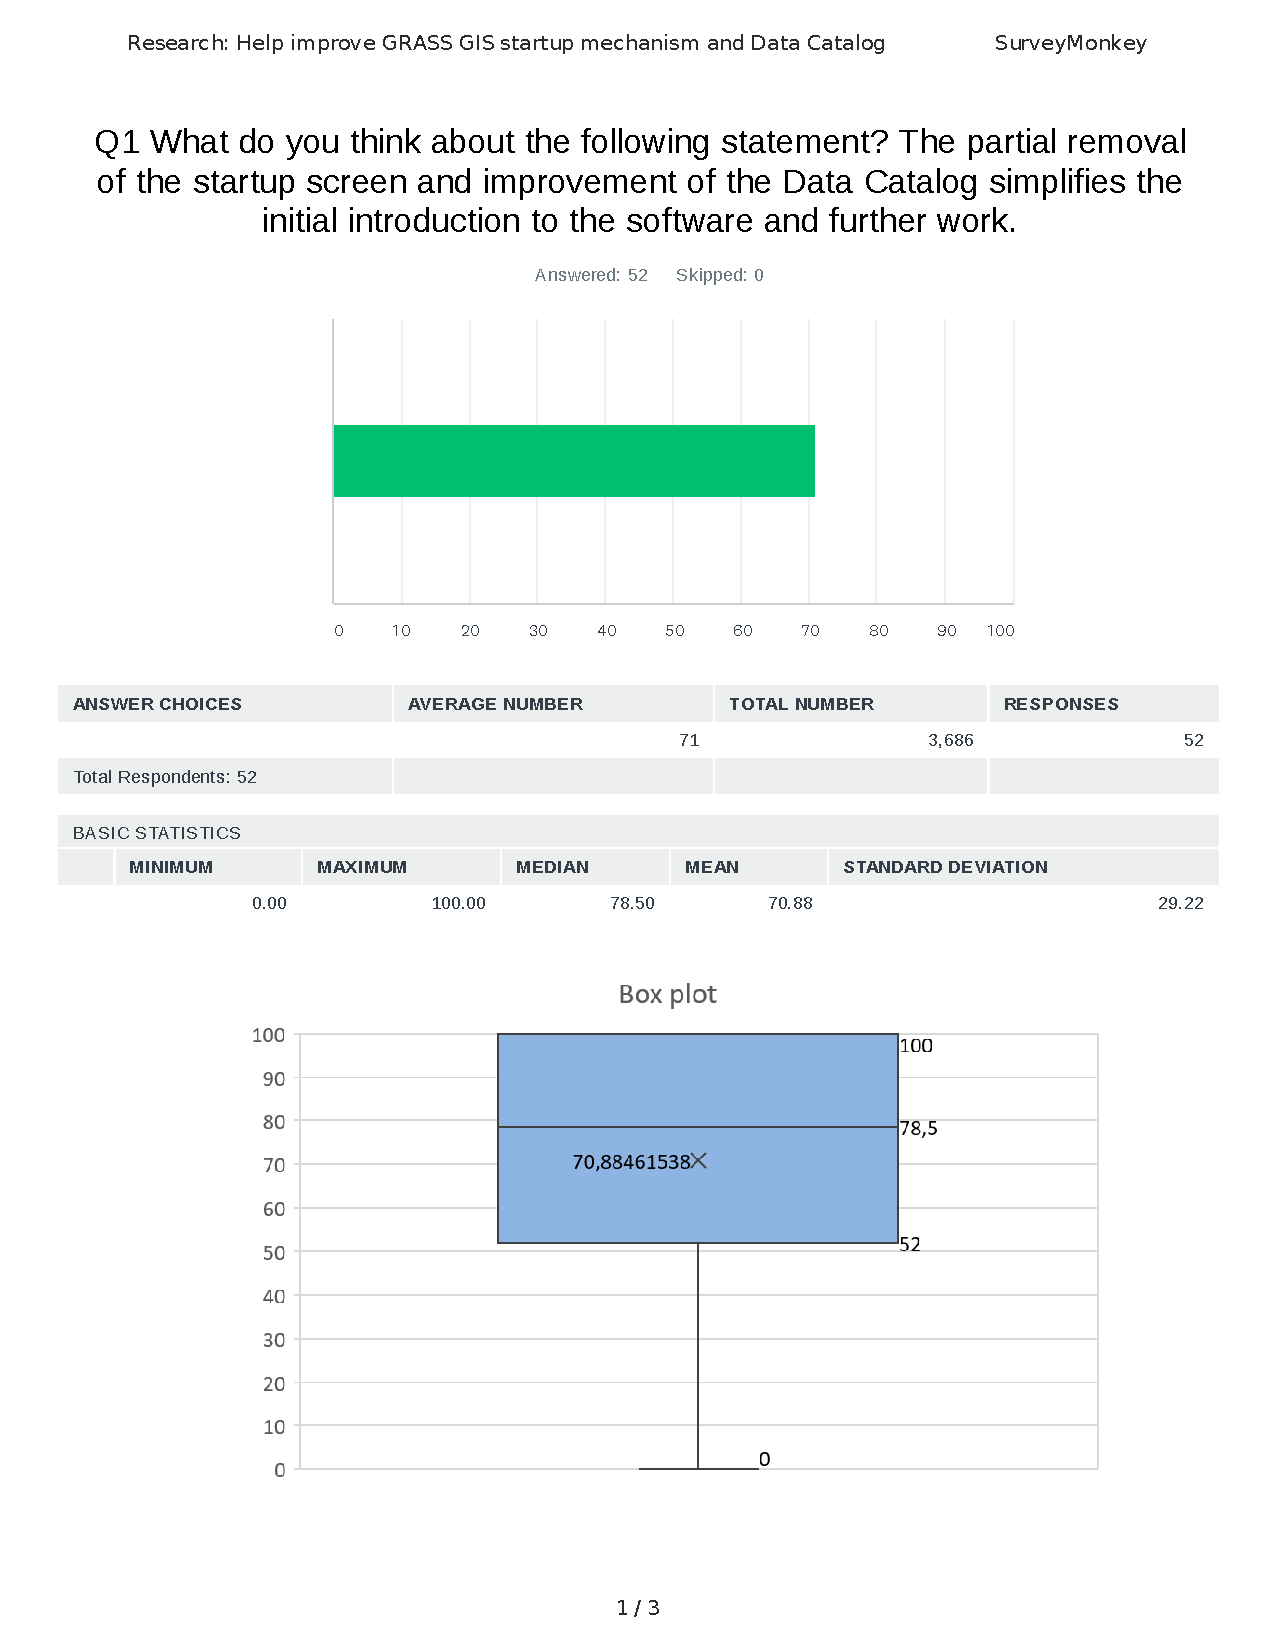
\includepdf[pages=-]{../pruzkumy/pruzkum_startup/celkove/Data_All_survey1_201101.pdf}

\section{ Research: Help create a better first-time user experience in GRASS GIS}

 \centering 
 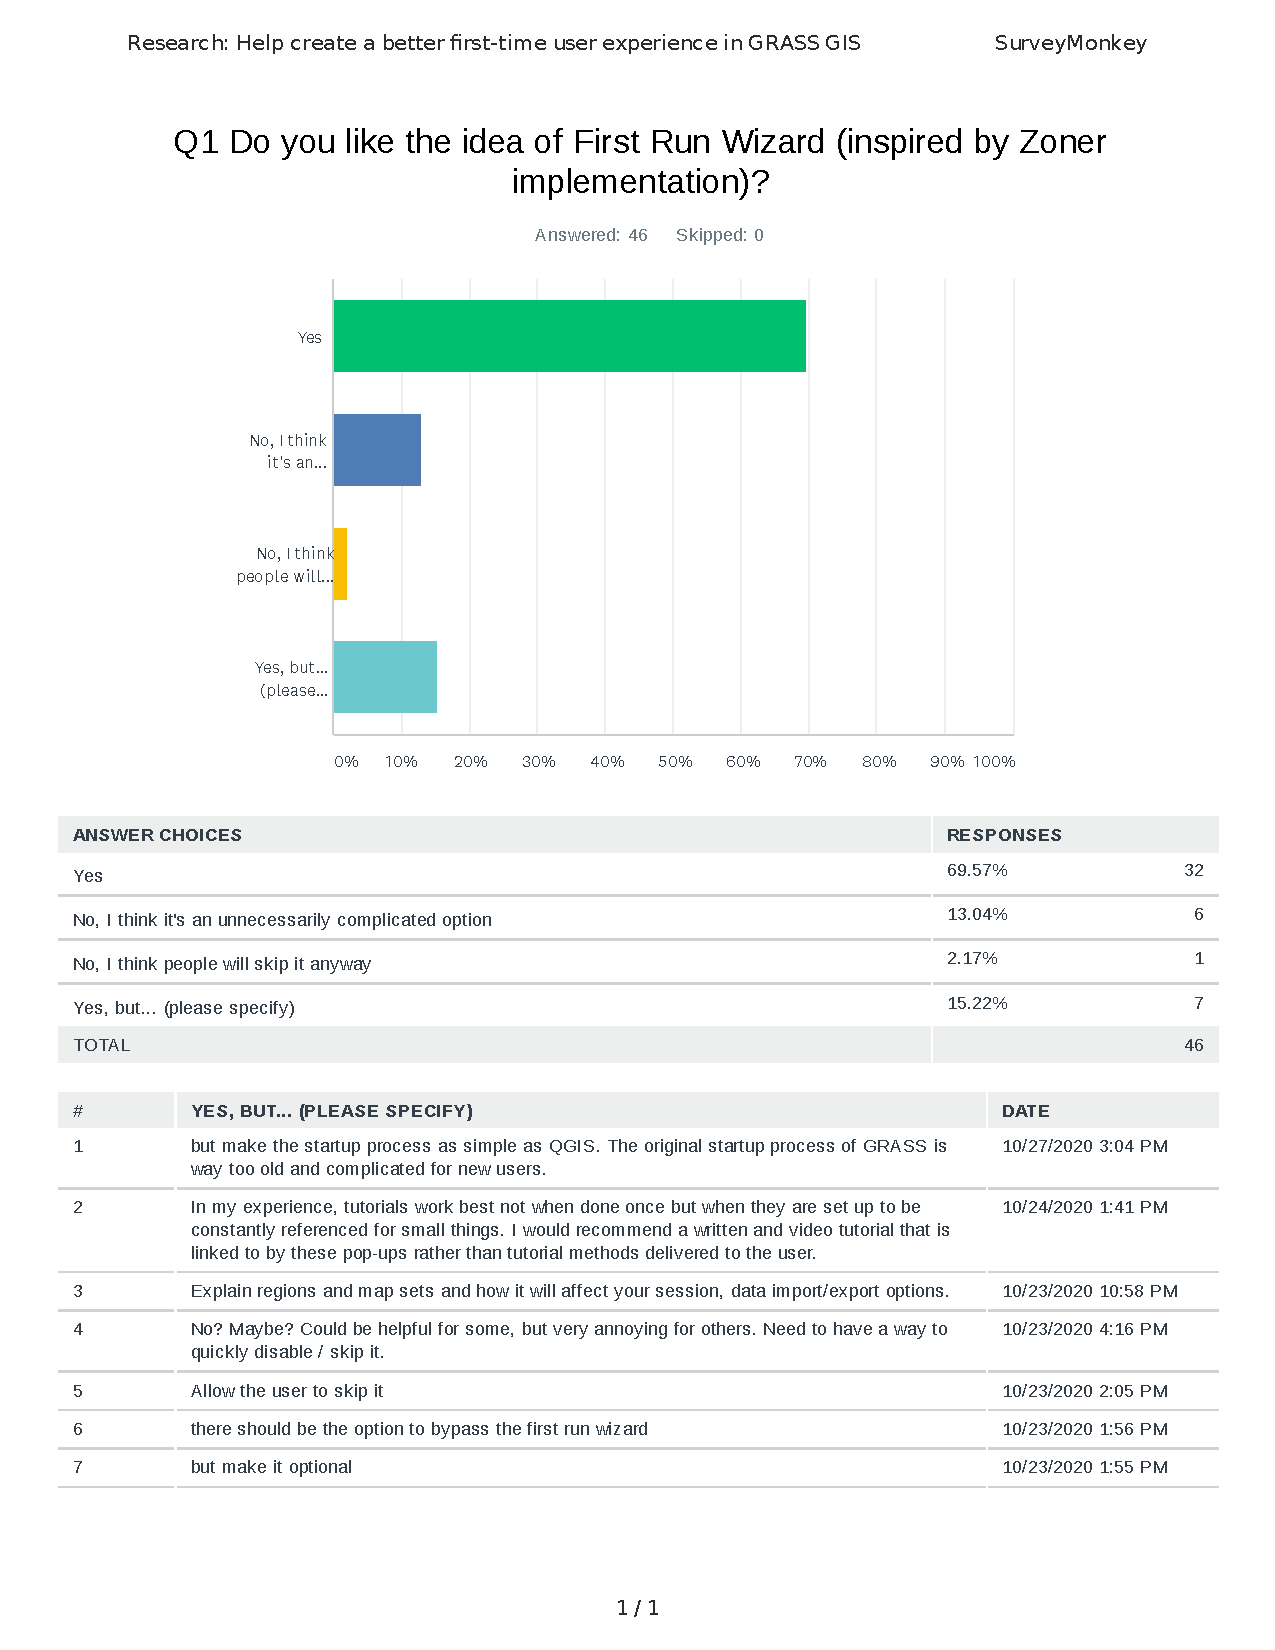
\includepdf[pages=-]{../pruzkumy/pruzkum_first_time/celkove/Data_All_survey2_201030.pdf}


\end{document}
